\begingroup
\setlength{\tabcolsep}{0pt}
%\renewcommand{\arraystretch}{0.55} % Default value: 1
%\setlength{\fboxsep}{1mm}
\begin{table*}[t]
\centering
\begin{tabular}{|P{2cm}|P{1.3cm}|P{2cm}|L{1.3cm} P{1.7cm} D |P{8cm}|}
\hline
Technique & Interval & Reduction & Data & AvgN$_{L2}$ & Cell  & \multirow{2}{*}{Scatter Plot} \\
& & & & & Side\% & \\
\hline
\multicolumn{6}{l}{\textbf{          Cloverleaf3D Proxy Hydrodynamics Application }} & \multirow{12}{*}{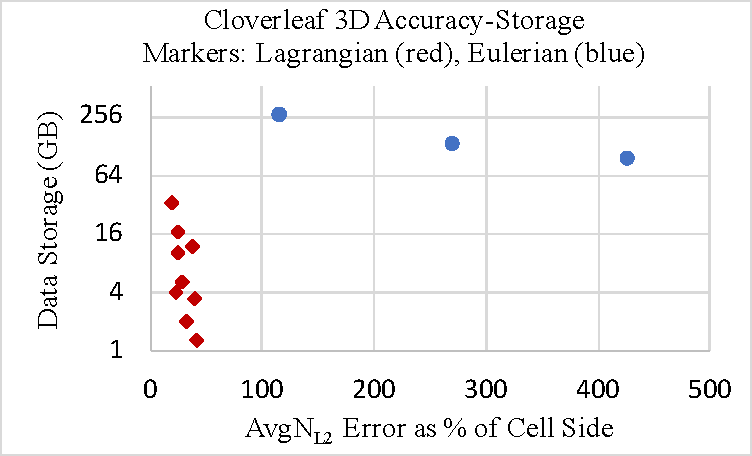
\includegraphics[width=0.95\linewidth]{images/cloverleaf_accuracy.pdf}}\\
\cline{1-6}
\multirow{3}{*}{Eulerian} & 20 & \multirow{3}{*}{Full Res} & 267 GB & 0.0197 & 116.17 &  \\
\cline{2-2}
& 40 & & 133 GB & 0.0459 & 270.49 & \\
\cline{2-2}
& 60 & & 95 GB & 0.0725 & 426.96 &  \\
\cline{1-6}
\multirow{9}{*}{Lagrangian} & \multirow{3}{*}{20} & 1:8 & 34 GB & 0.0032 & 18.928 & \\
\cline{3-3}
 & & 1:27 & 10 GB & 0.0040 & 23.891 & \\
\cline{3-3}
 & & 1:64 & 4 GB & 0.0040 & 23.583 & \\
\cline{2-3}
& \multirow{3}{*}{40} & 1:8 & 17 GB & 0.0043 & 25.646 &  \\
\cline{3-3}
& & 1:27 & 5.1 GB & 0.0049 & 29.145 &  \\
\cline{3-3}
& & 1:64 & 2 GB & 0.0053 & 31.353 & \\
\cline{2-3}
& \multirow{3}{*}{60} & 1:8 & 12 GB & 0.0064 & 37.882 & \\
\cline{3-3}
& & 1:27 & 3.4 GB & 0.0066 & 39.002 & \multirow{6}{*}{\raisebox{-33.5mm}[0pt][0pt]{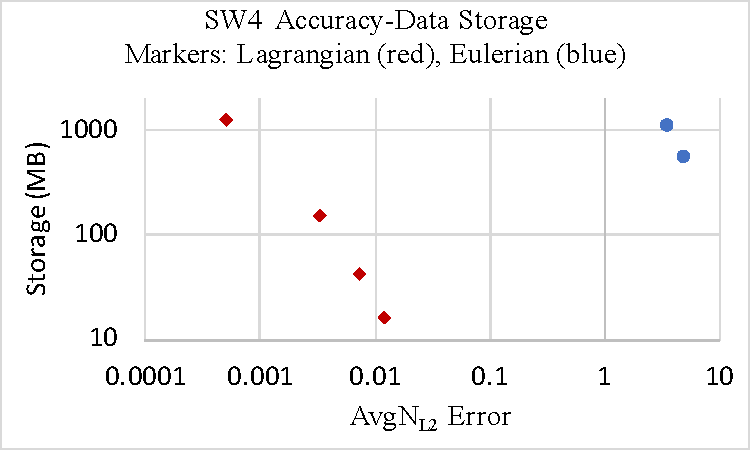
\includegraphics[width=0.95\linewidth]{images/sw4_accuracy.pdf}}} \\
\cline{3-3}
& & 1:64 & 1.3 GB & 0.0070 & 41.247 & \\
\cline{1-6}
\multicolumn{6}{l}{\textbf{          SW4 Seismic Wave Modeling Simulation }} &  \\
\cline{1-6}
\multirow{2}{*}{Eulerian} & 250 & \multirow{2}{*}{Full Res} & 1100 MB & 3.5714 & 0.9224 & \\
\cline{2-2}
 & 500 & & 550 MB & 5.0493 & 1.3023  & \\
\cline{1-6}
\multirow{4}{*}{Lagrangian} & \multirow{4}{*}{250} & 1:1 & 1300 MB & 0.0005 & 0.0001  &  \\
\cline{3-3}
 &  & 1:8 & 158 MB & 0.0033 & 0.0008 &  \\
\cline{3-3}
 &  & 1:27 & 42 MB & 0.0072 & 0.0018 & \\
\cline{3-3}
 &  & 1:64 & 16 MB & 0.0128 & 0.0031 &  \\
\cline{1-6}
\multicolumn{6}{l}{\textbf{          Nyx Cosmology Simulation }} & \\
\cline{1-6}
\multirow{4}{*}{Eulerian} & 25 & \multirow{4}{*}{Full Res} & 227 MB & 0.010 & 2.2954 &  \\
\cline{2-2}%\cline{4-6}
& 50 & & 120 MB & 0.037 & 8.4090 &  \multirow{16}{*}{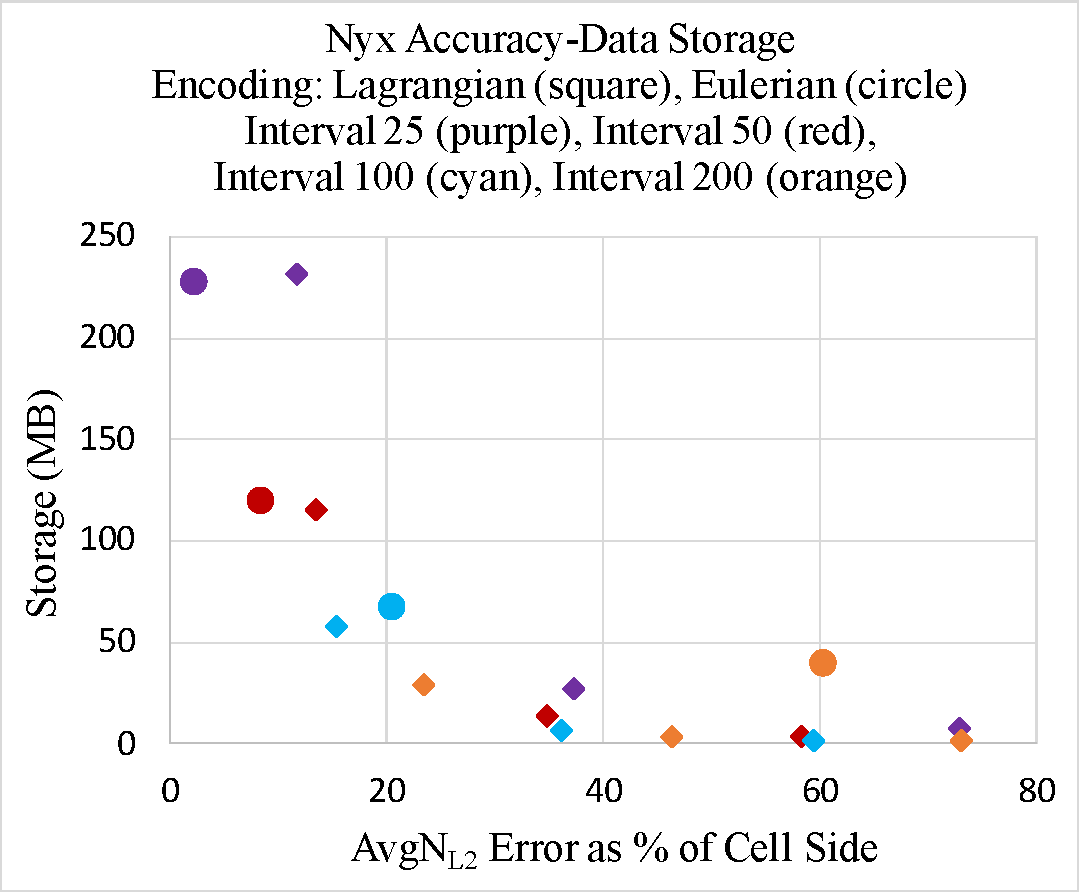
\includegraphics[width=0.95\linewidth]{images/nyx_accuracy.pdf}}\\
\cline{2-2}%\cline{4-6}
& 100 & & 67 MB & 0.090 & 20.454 & \\
\cline{2-2}%\cline{4-6}
& 200 & & 40 MB & 0.265 & 60.227 & \\
\cline{1-6}
\multirow{12}{*}{Lagrangian} & \multirow{3}{*}{25} & 1:1 & 232 MB & 0.051 & 11.613 & \\
\cline{3-3}
& & 1:8 & 27 MB & 0.164 & 37.272 &  \\
\cline{3-3}
& & 1:27 & 8 MB & 0.320 & 72.727 &  \\
\cline{2-3}
& \multirow{3}{*}{50} & 1:1 & 166 MB & 0.059 & 13.409 & \\
\cline{3-3}
& & 1:8 & 14 MB & 0.153 & 34.772 &  \\
\cline{3-3}
& & 1:27 & 4 MB & 0.256 & 58.181 &  \\
\cline{2-3}
& \multirow{3}{*}{100} & 1:1 & 58 MB & 0.067 & 15.227 &  \\
\cline{3-3}
& & 1:8 & 7 MB & 0.159 & 36.136 &  \\
\cline{3-3}
& & 1:27 & 2 MB & 0.261 & 59.318 & \\
\cline{2-3}
 & \multirow{3}{*}{200} & 1:1 & 29 MB & 0.103 & 23.409 &  \\
\cline{3-3}
& & 1:8 & 3.4 MB & 0.204 & 46.363 & \\
\cline{3-3}
& & 1:27 & 1 MB & 0.321 & 72.954 &  \\
\hline
\end{tabular}
\vspace{-3mm}
\caption{\textit{Post hoc} efficacy evaluation and experiment configurations for our three simulation codes.}
\label{table:accuracy}
\vspace{-5mm}
\end{table*}
\endgroup

\begin{figure*}
\begin{subfigure}{0.195\textwidth}
\centering
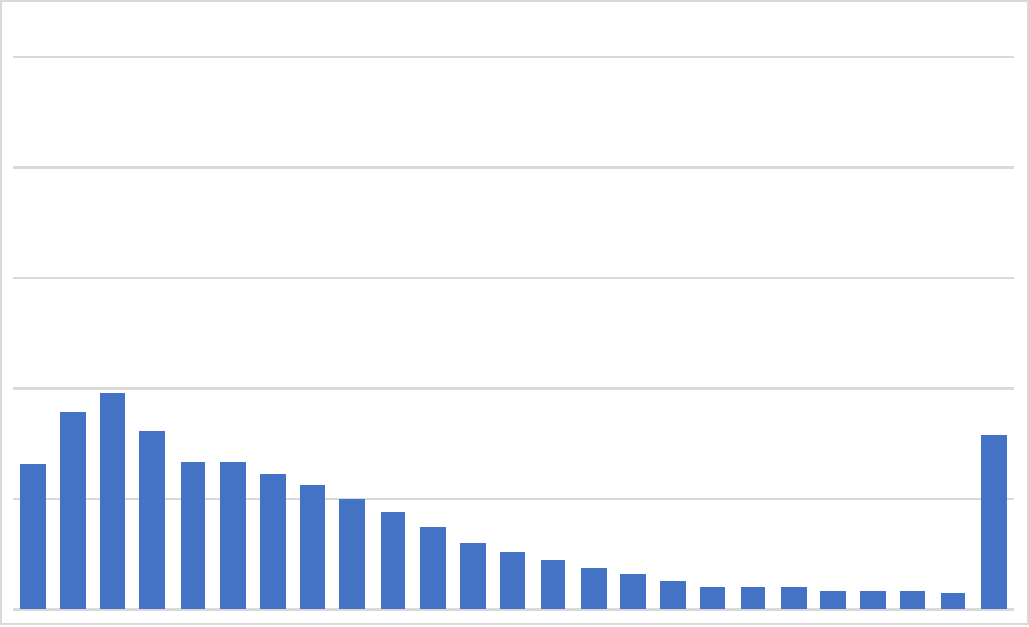
\includegraphics[width=0.9\linewidth]{results/cloverleaf3d/eul_1/Eul1_AvgL2.pdf}
\vspace{-2mm}
\caption{Eul 20 Avg$_{L2}$ L2 }
\end{subfigure}
\begin{subfigure}{0.195\textwidth}
\centering
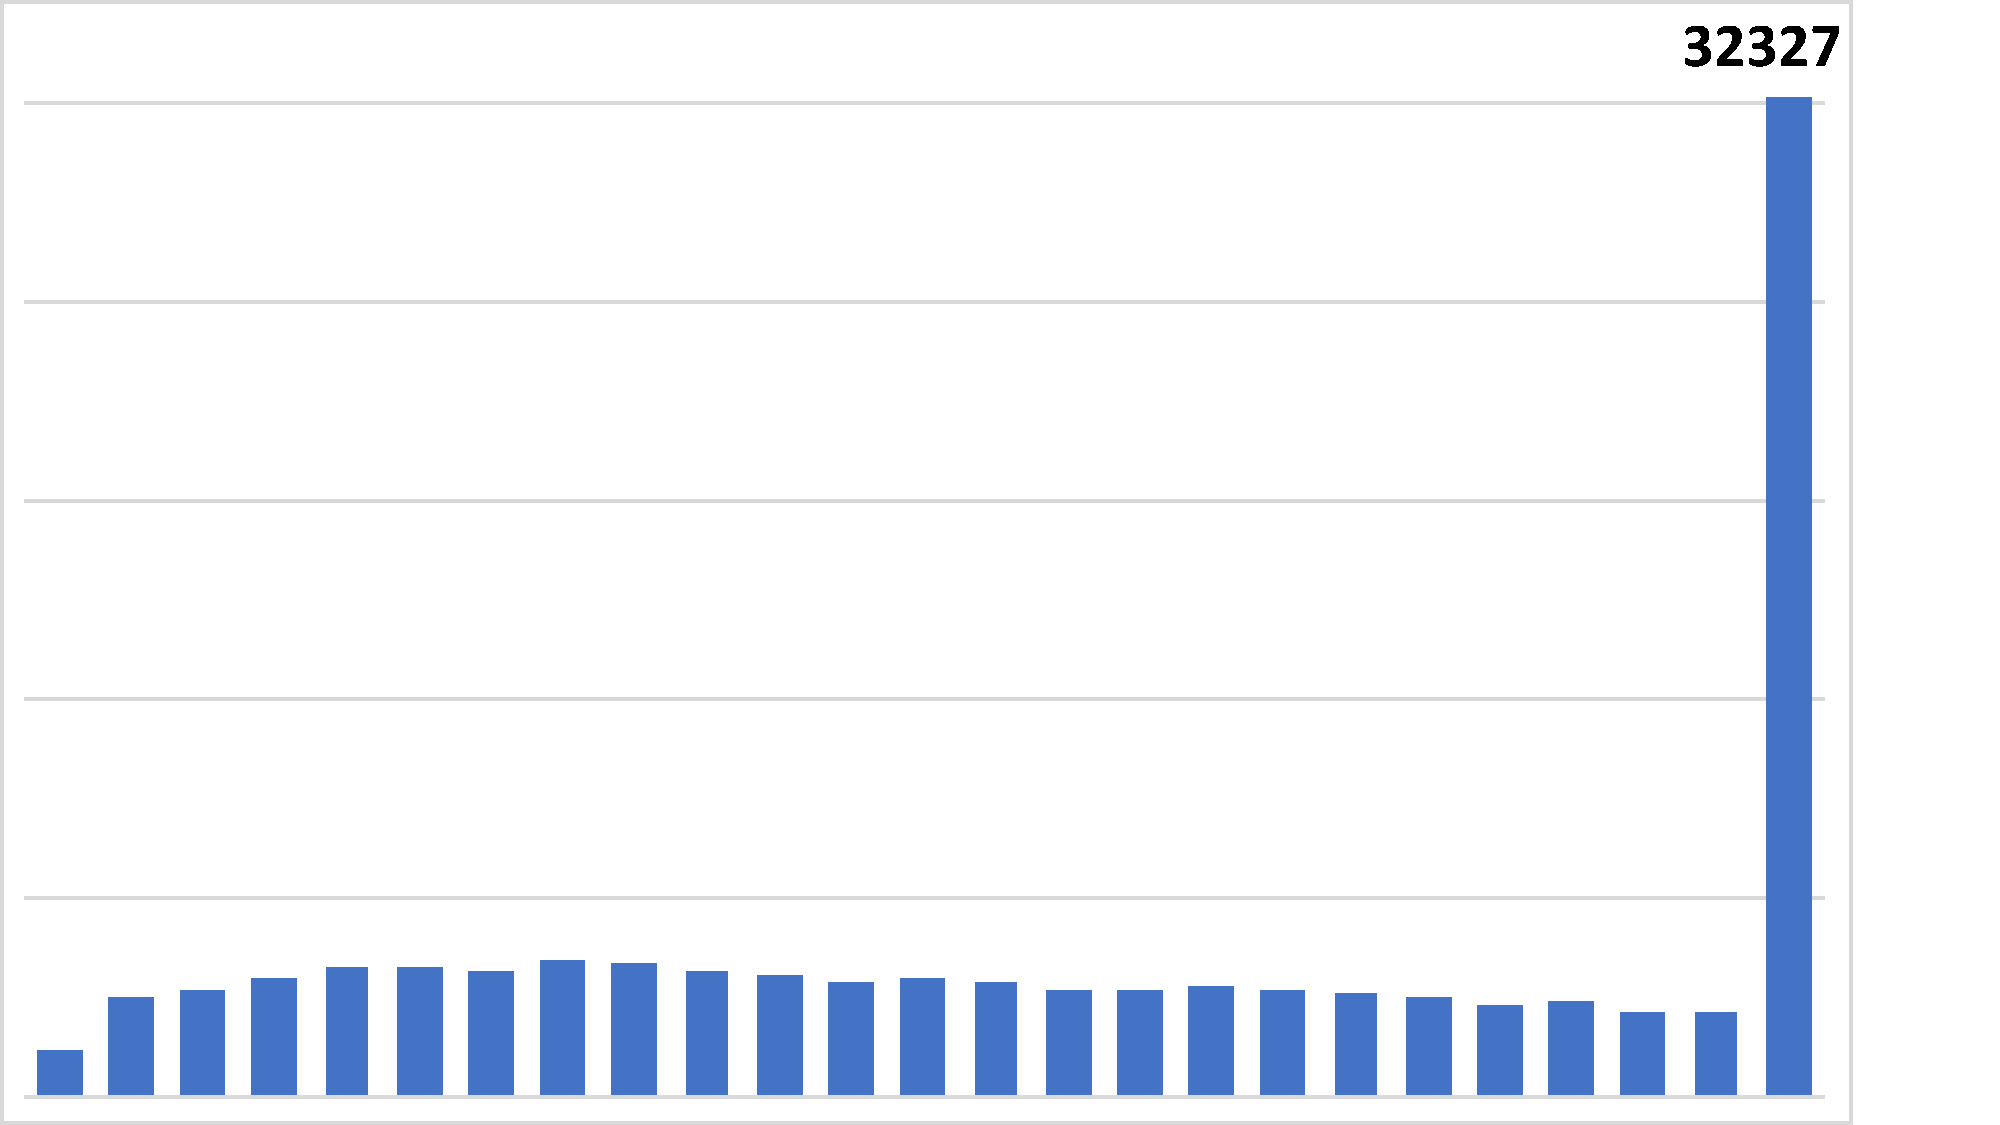
\includegraphics[width=0.95\linewidth]{results/cloverleaf3d/eul_2/Eul2_AvgL2.pdf}
\vspace{-2mm}
\caption{Eul 40 Avg$_{L2}$ L2 }
\end{subfigure}
\begin{subfigure}{0.195\textwidth}
\centering
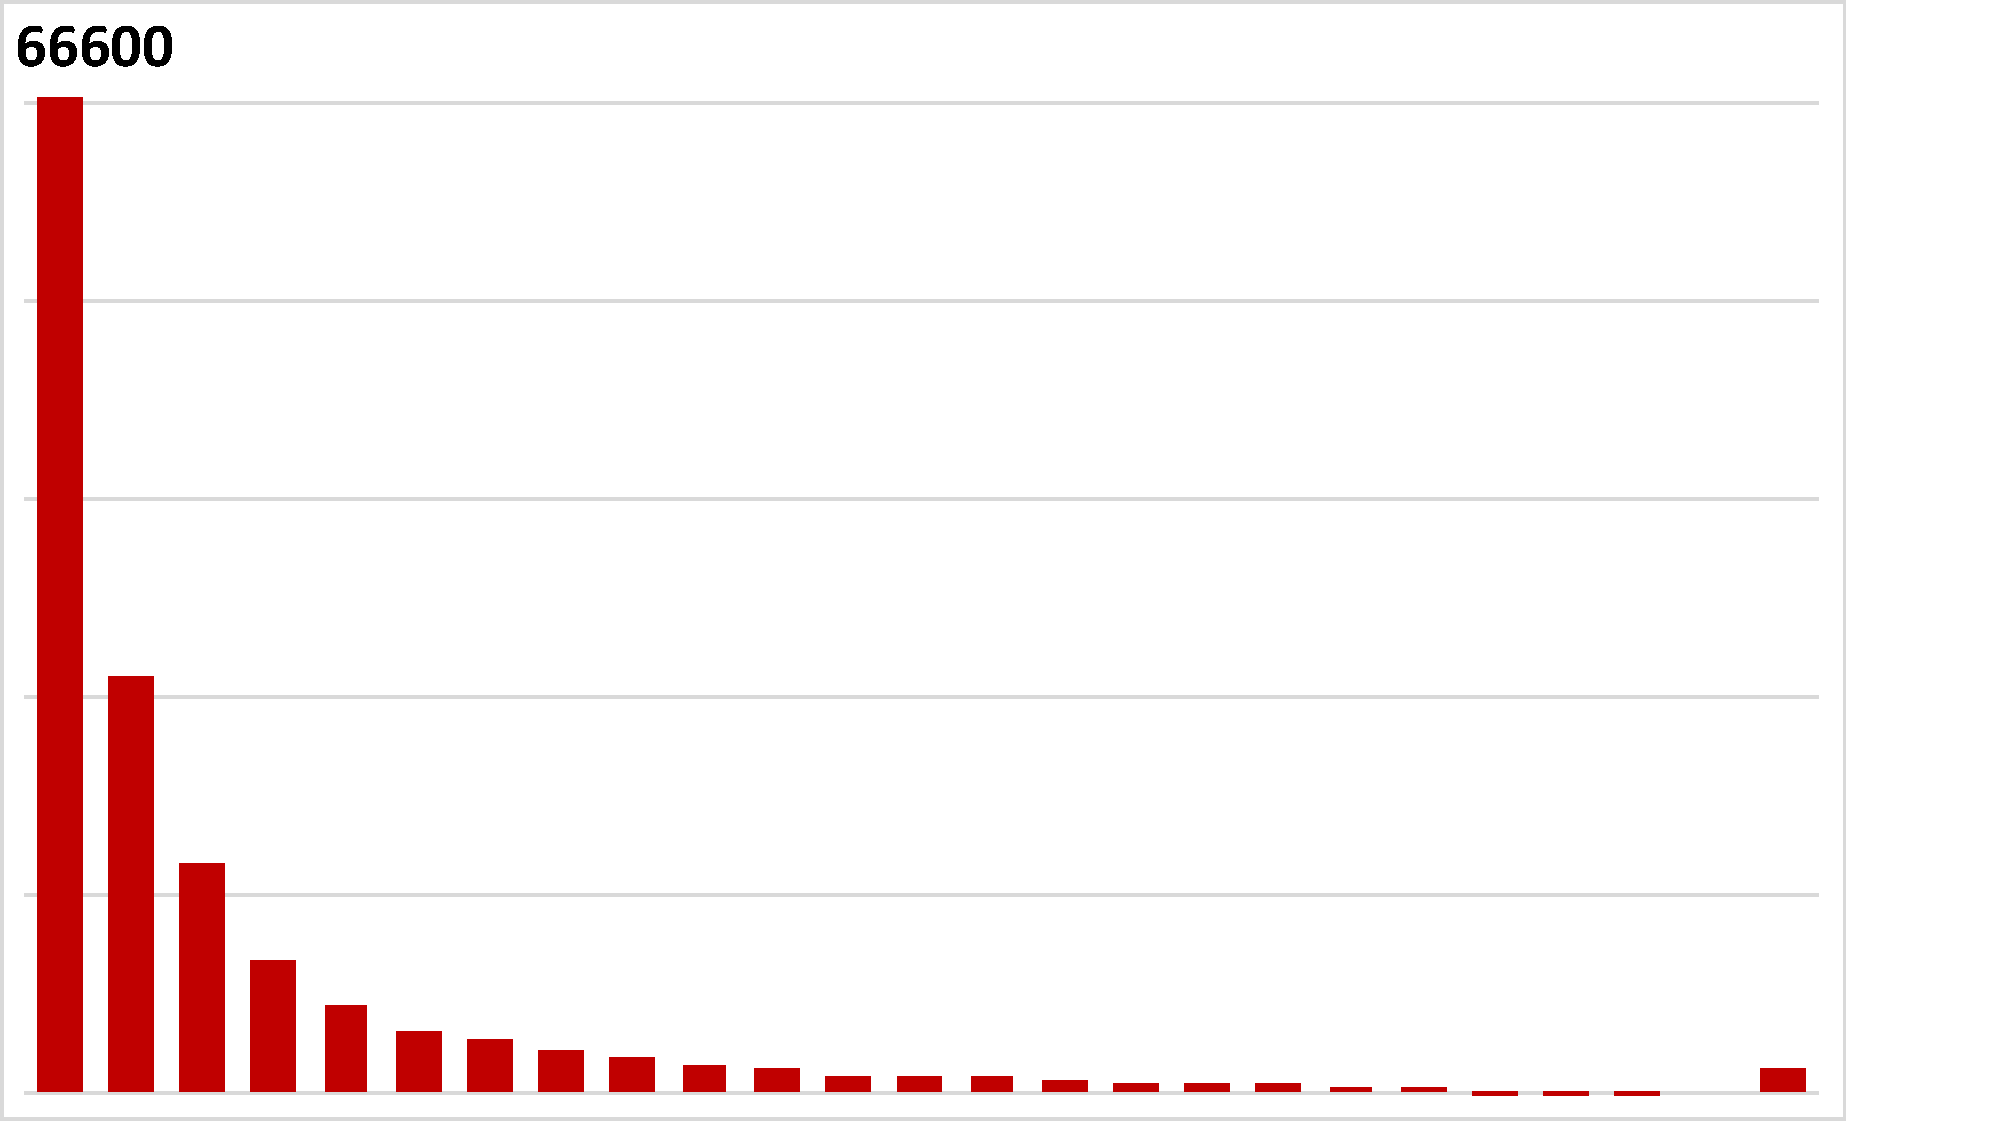
\includegraphics[width=0.9\linewidth, trim={0cm 0cm 2.5cm 0cm}, clip]{results/cloverleaf3d/lag_4/Lag4_AvgL2.pdf}
\vspace{-2mm}
\caption{Lag 40 1:8 Avg$_{L2}$ }
\end{subfigure}
\begin{subfigure}{0.195\textwidth}
\centering
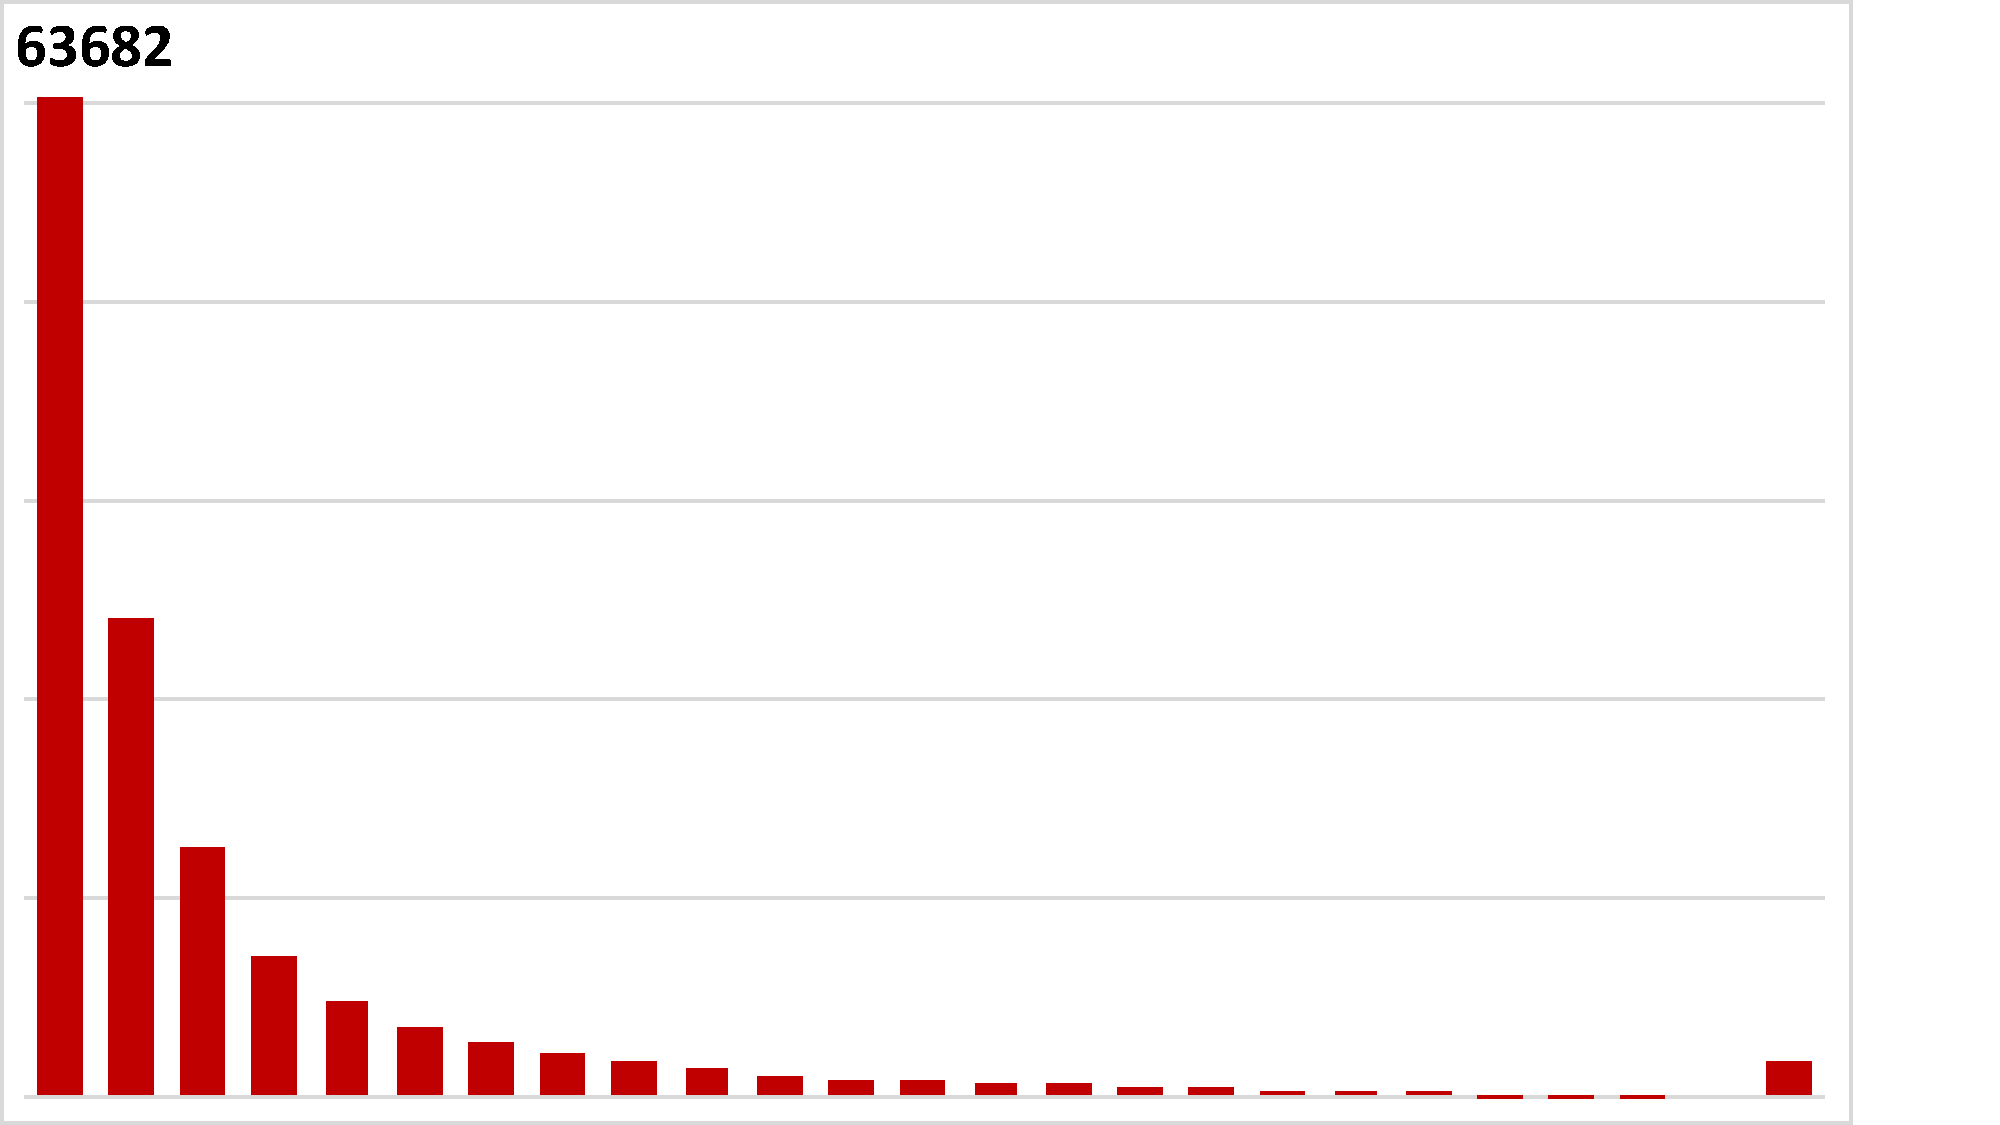
\includegraphics[width=0.9\linewidth, trim={0cm 0cm 2.5cm 0cm}, clip]{results/cloverleaf3d/lag_5/Lag5_AvgL2.pdf}
\vspace{-2mm}
\caption{Lag 40 1:27 Avg$_{L2}$ }
\end{subfigure}
\begin{subfigure}{0.195\textwidth}
\centering
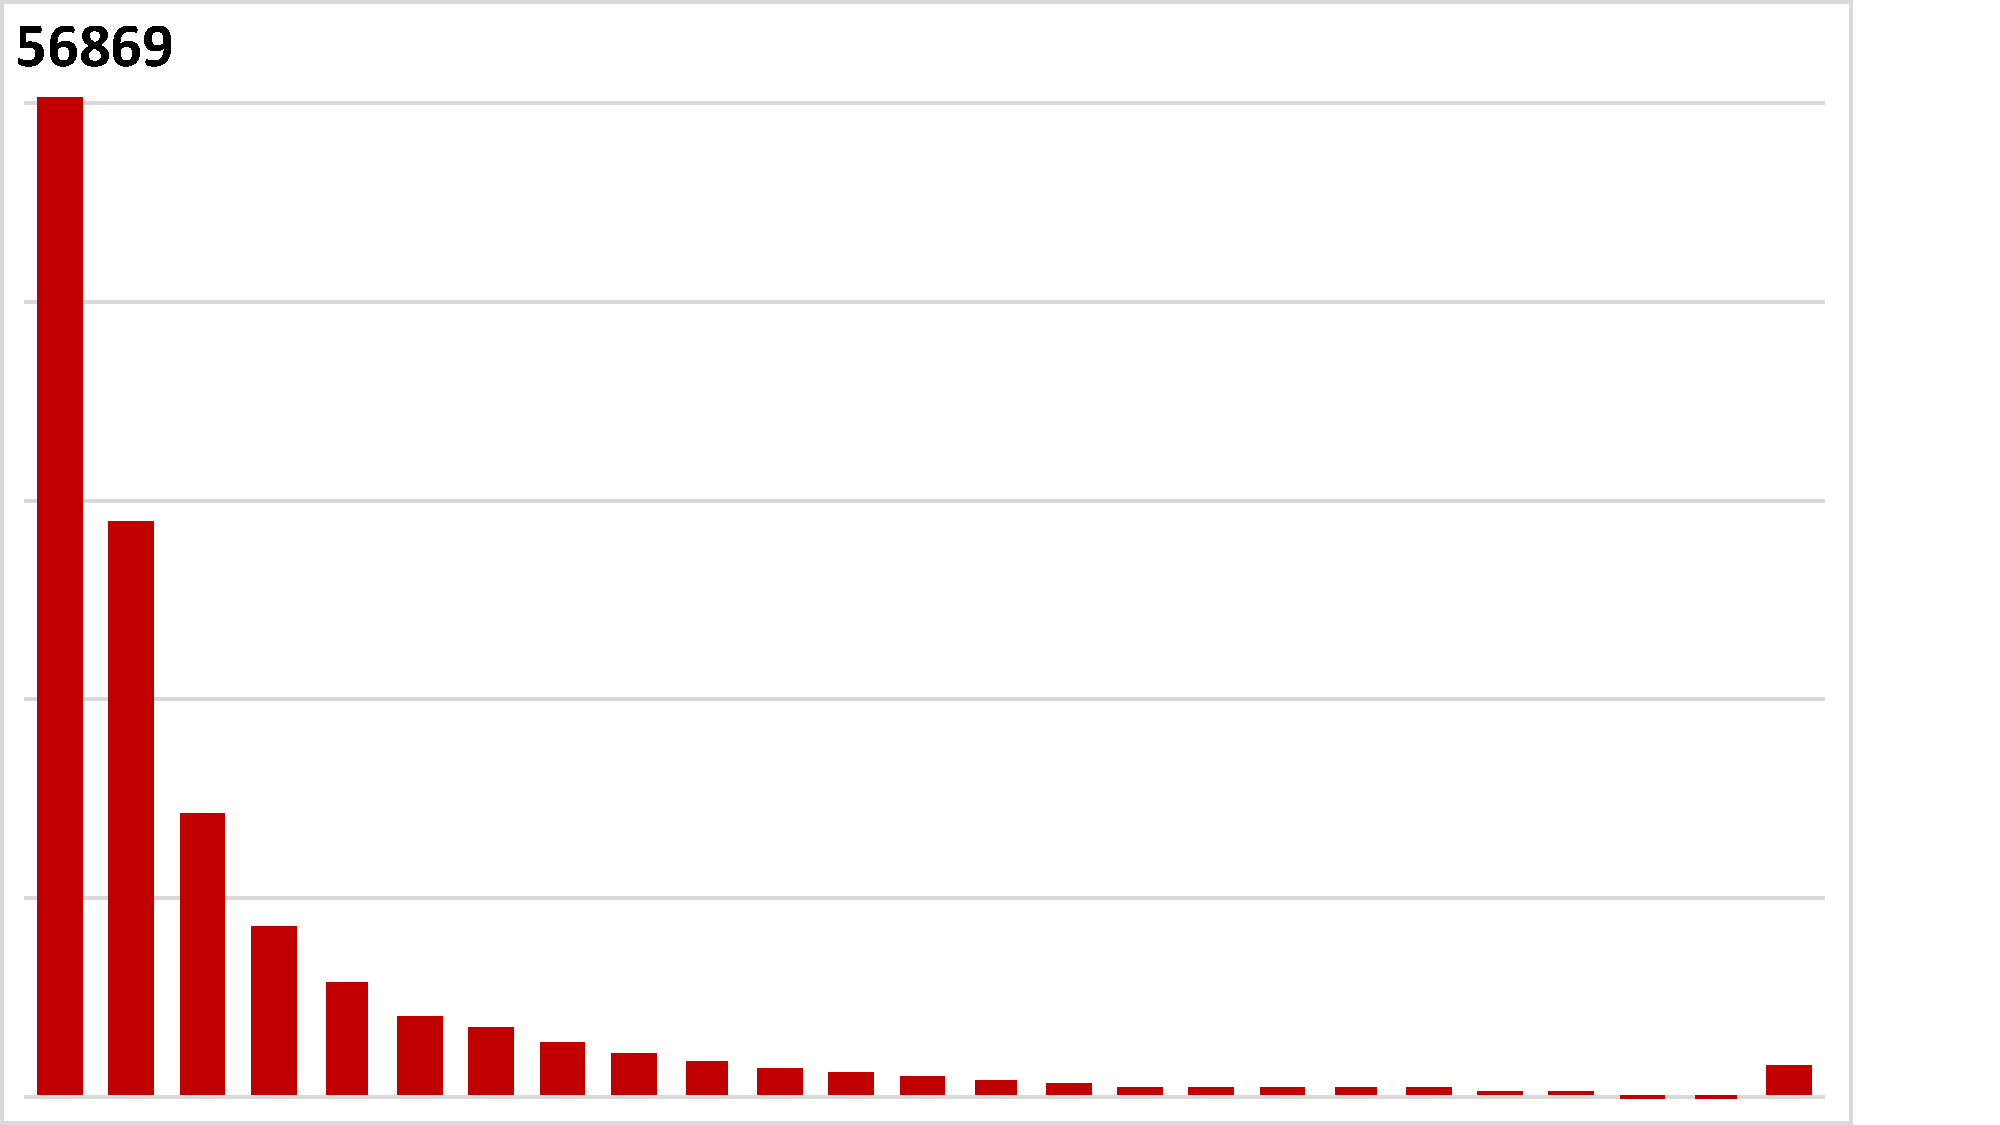
\includegraphics[width=0.9\linewidth, trim={0cm 0cm 2.5cm 0cm}, clip]{results/cloverleaf3d/lag_6/Lag6_AvgL2.pdf}
\vspace{-2mm}
\caption{Lag 40 1:64 Avg$_{L2}$ }
\end{subfigure}
\begin{subfigure}{0.195\textwidth}
\centering
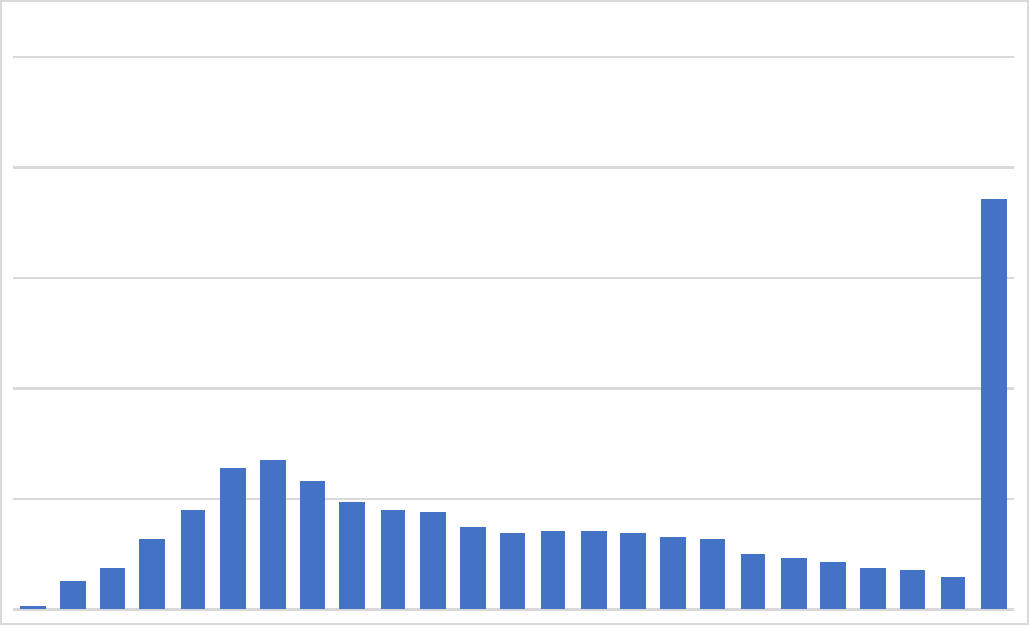
\includegraphics[width=0.9\linewidth]{results/cloverleaf3d/eul_1/Eul1_Max.pdf}
\vspace{-2mm}
\caption{Eul 20 Max$_{L2}$ }
\end{subfigure}
\begin{subfigure}{0.195\textwidth}
\centering
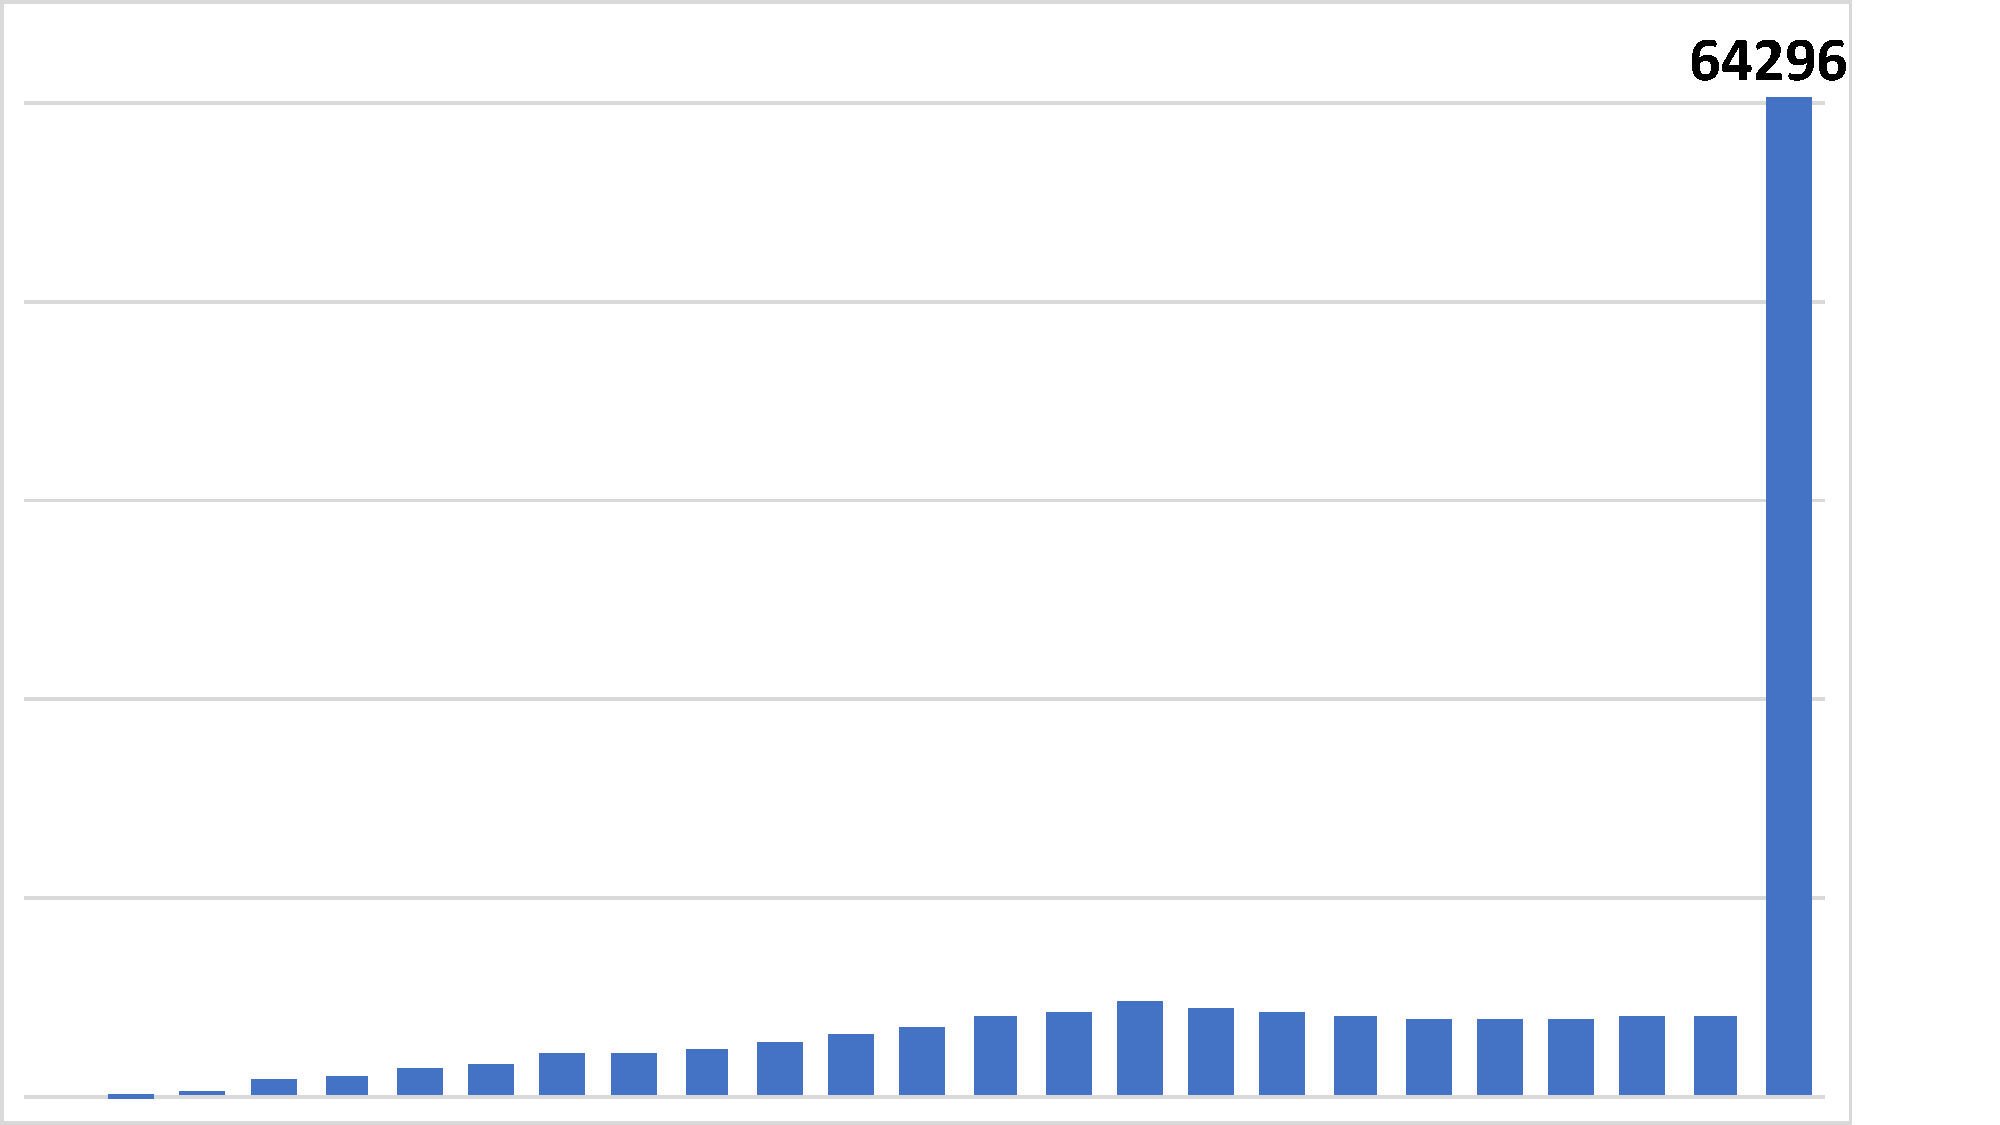
\includegraphics[width=0.95\linewidth]{results/cloverleaf3d/eul_2/Eul2_Max.pdf}
\vspace{-2mm}
\caption{Eul 40 Max$_{L2}$ }
\end{subfigure}
\hspace{0.2mm}
\begin{subfigure}{0.195\textwidth}
\centering
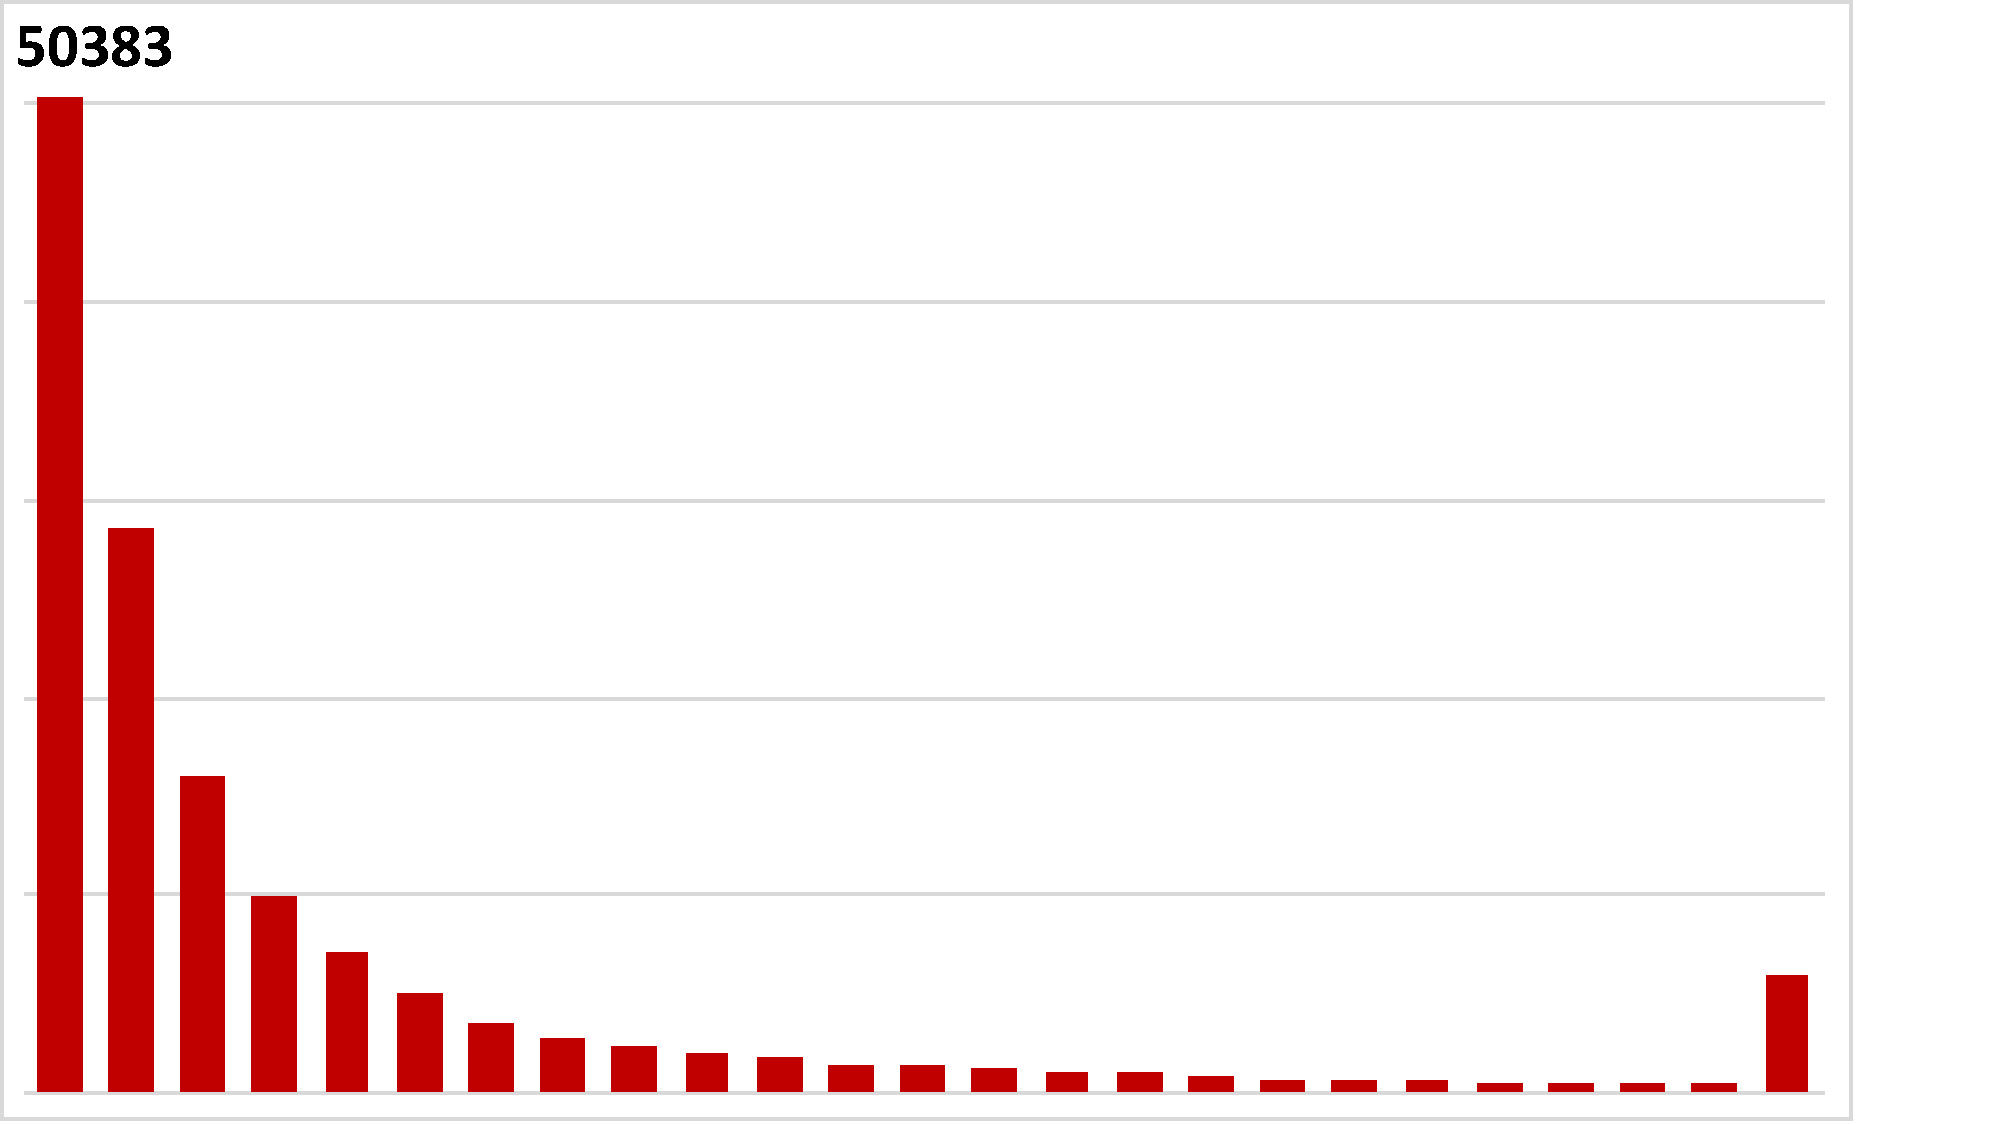
\includegraphics[width=0.9\linewidth, trim={0cm 0cm 2.5cm 0cm}, clip]{results/cloverleaf3d/lag_4/Lag4_Max.pdf}
\vspace{-2mm}
\caption{Lag 40 1:8 Max$_{L2}$ }
\end{subfigure}
\begin{subfigure}{0.195\textwidth}
\centering
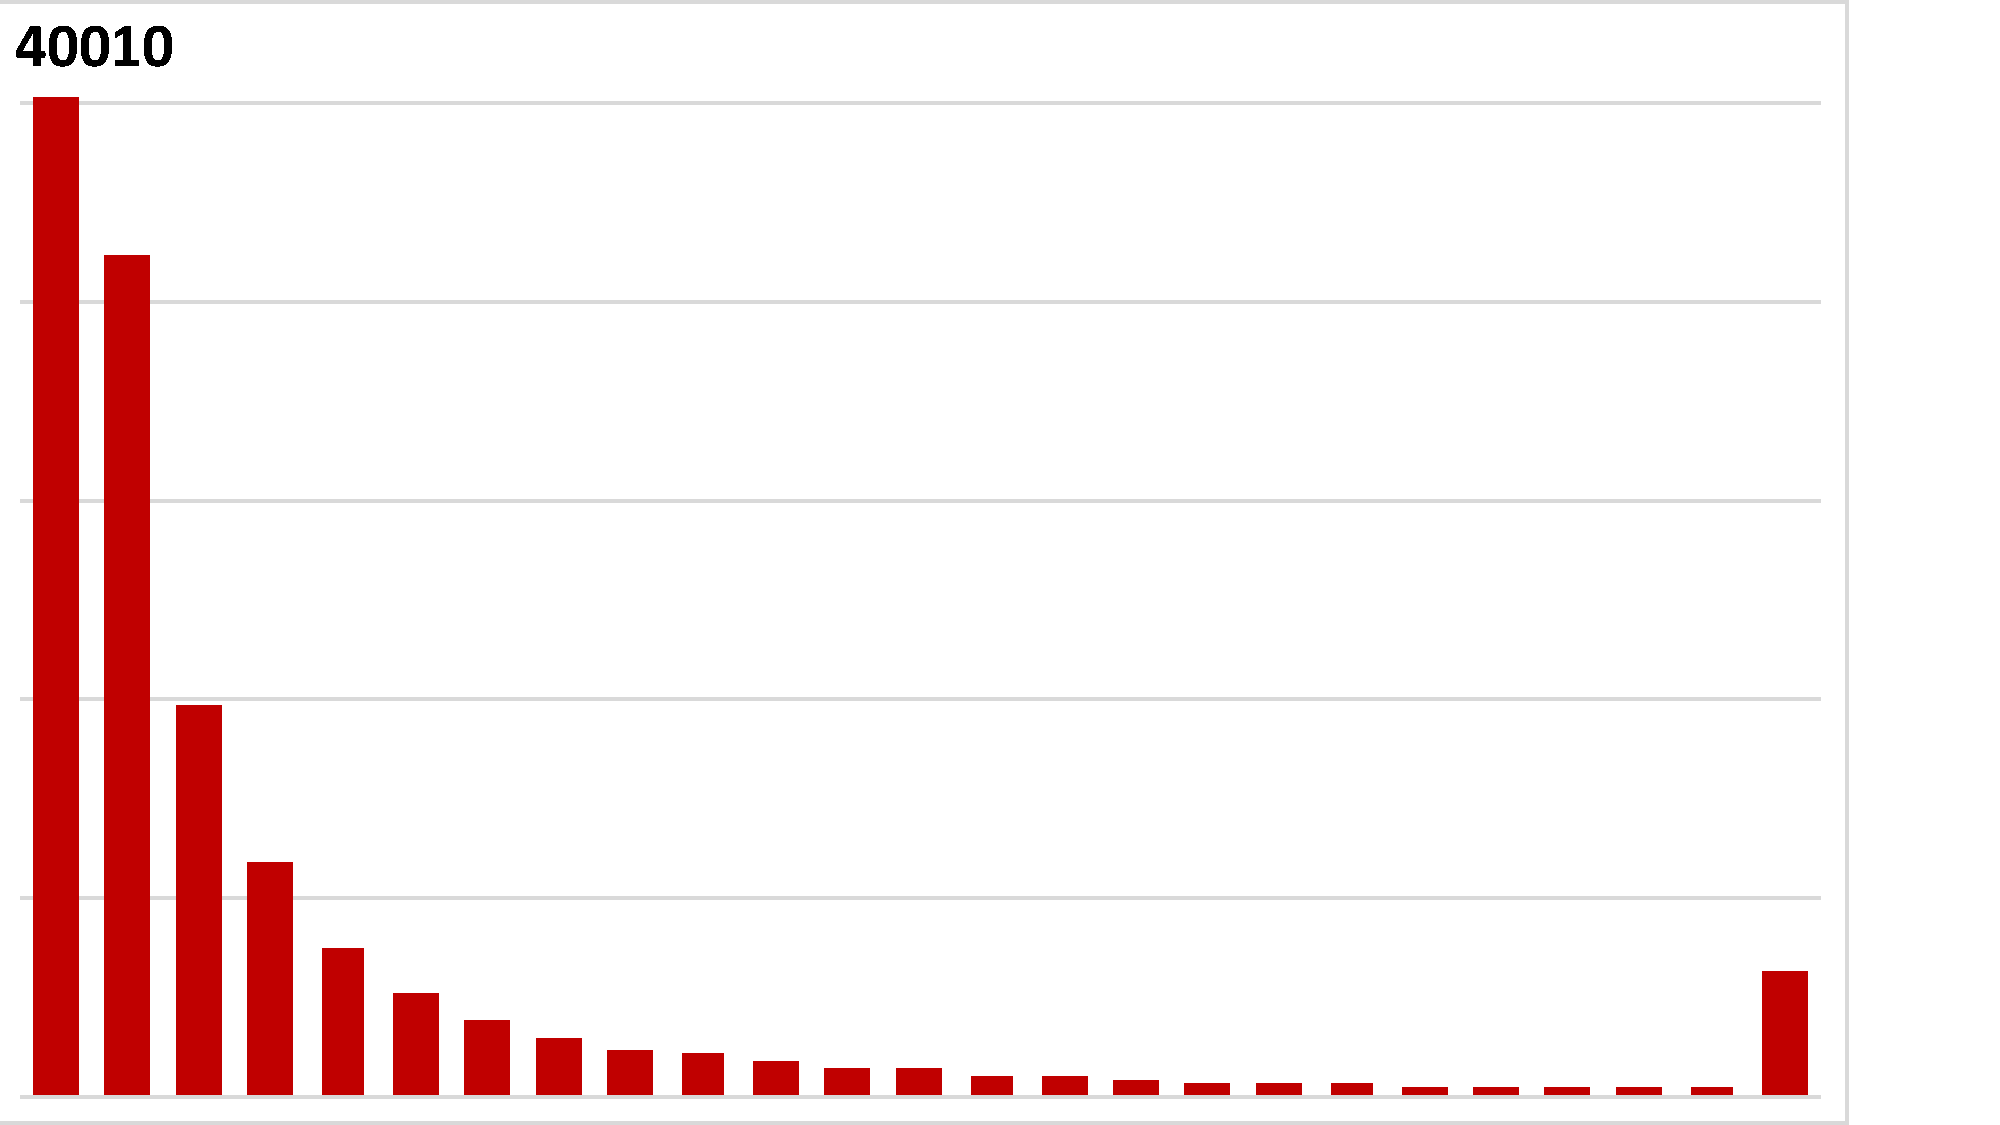
\includegraphics[width=0.9\linewidth, trim={0cm 0cm 2.5cm 0cm}, clip]{results/cloverleaf3d/lag_5/Lag5_Max.pdf}
\vspace{-2mm}
\caption{Lag 40 1:27 Max$_{L2}$}
\end{subfigure}
\begin{subfigure}{0.195\textwidth}
\centering
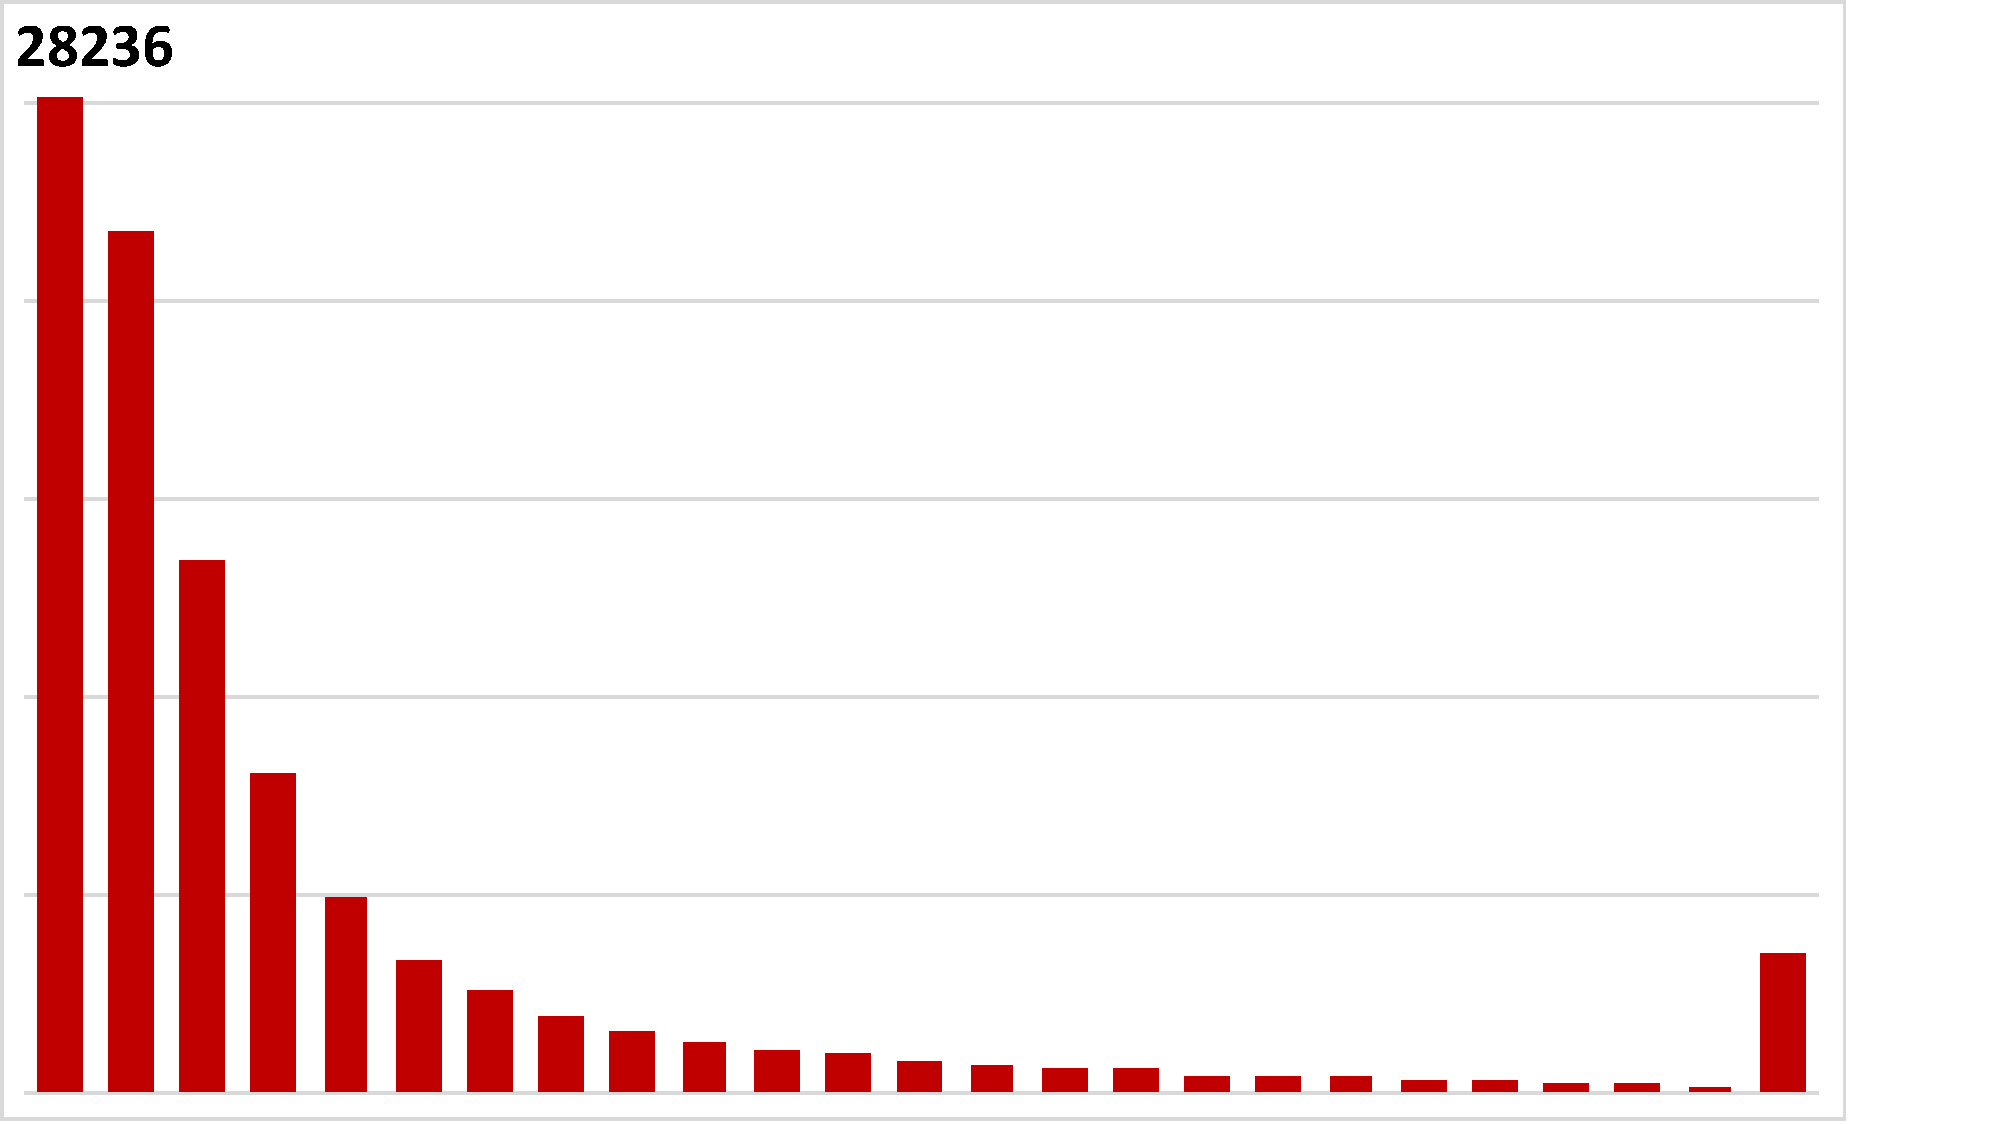
\includegraphics[width=0.9\linewidth, trim={0cm 0cm 2.5cm 0cm}, clip]{results/cloverleaf3d/lag_6/Lag6_Max.pdf}
\vspace{-2mm}
\caption{Lag 40 1:64 Max$_{L2}$}
\end{subfigure}
%\begin{subfigure}{0.24\textwidth}
%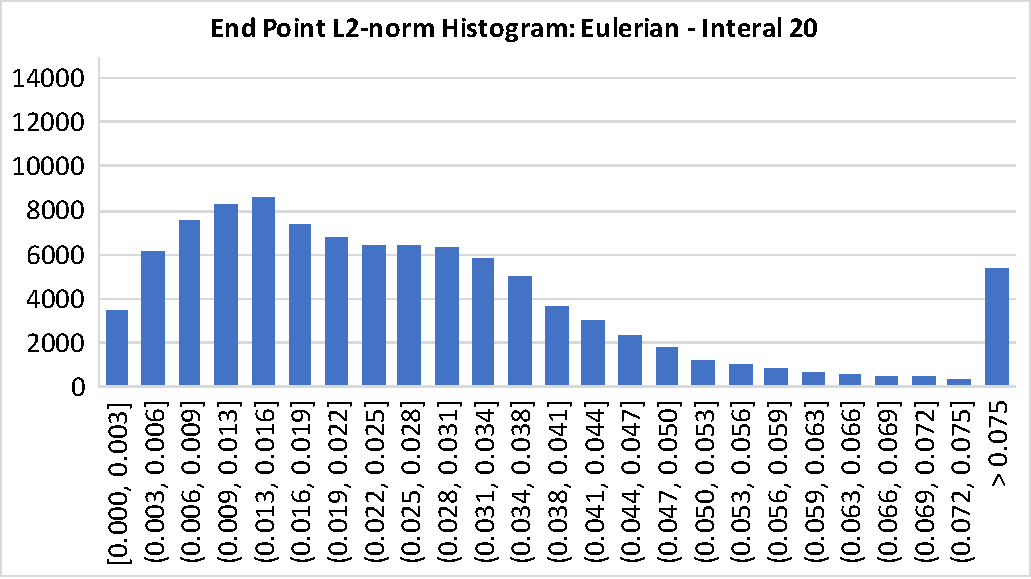
\includegraphics[width=0.9\linewidth]{results/cloverleaf3d/eul_1/Eul1_EndPt.pdf}
%\caption{Eulerian 20 End Point}
%\end{subfigure}
%\hspace{1mm}
%\begin{subfigure}{0.21\textwidth}
%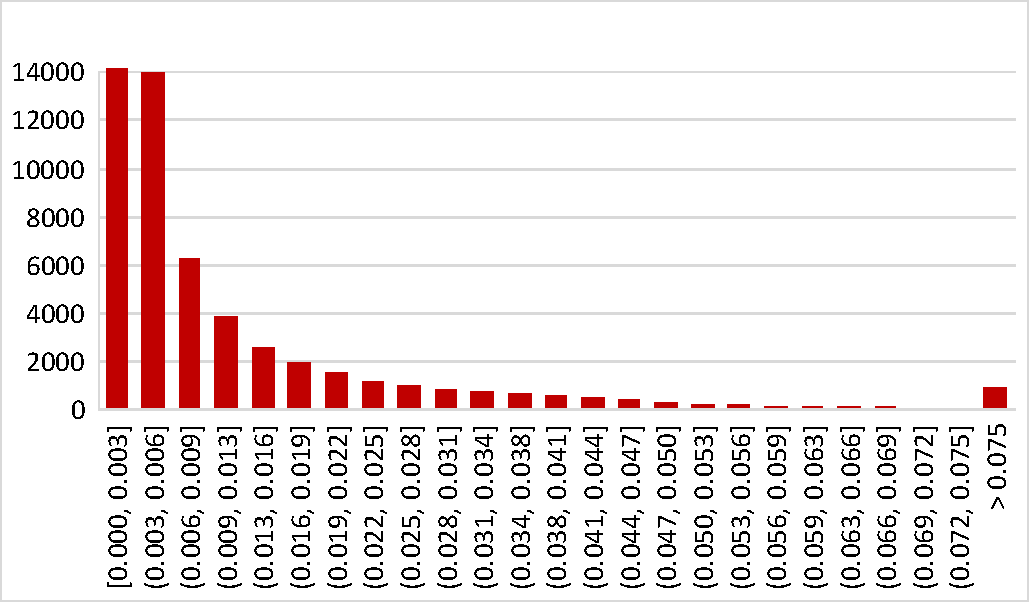
\includegraphics[width=1\linewidth]{results/cloverleaf3d/lag_4/Lag4_EndPt.pdf}
%\caption{Lagrangian 40 1:8 End Point}
%\end{subfigure}
%\hspace{1mm}
%\begin{subfigure}{0.21\textwidth}
%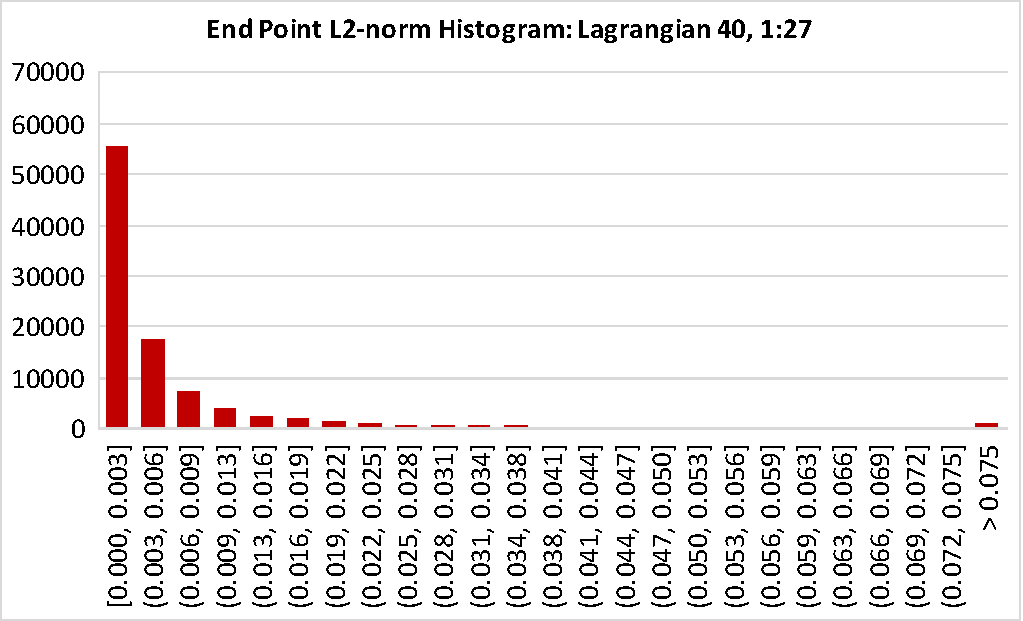
\includegraphics[width=1\linewidth]{results/cloverleaf3d/lag_5/Lag5_EndPt.pdf}
%\caption{Lagrangian 40 1:27 End Point}
%\end{subfigure}
%\hspace{1mm}
%\begin{subfigure}{0.21\textwidth}
%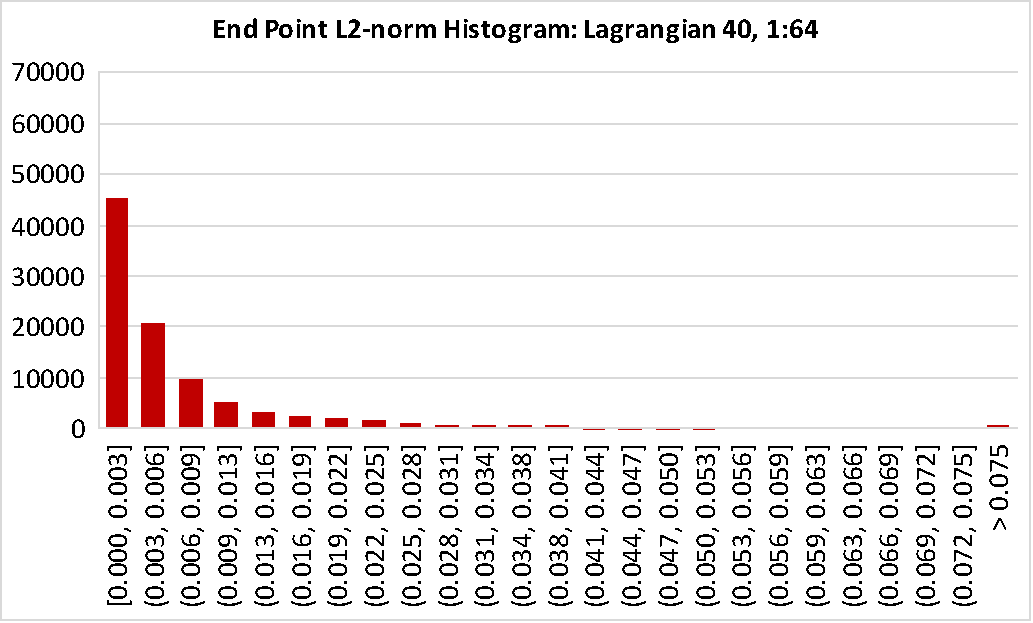
\includegraphics[width=1\linewidth]{results/cloverleaf3d/lag_6/Lag6_EndPt.pdf}
%\caption{Lagrangian 40 1:64 End Point}
%\end{subfigure}
\vspace{-3mm}
\caption{\textbf{Cloverleaf3D} experiment histograms for 100,000 test particle interpolation errors. Each plot has 25 bins, ranging from 0 to $>$0.05, with bar height encoding number of particles. Horizontal grid lines mark increments of 5,000.} 
\label{fig:clover_histograms}
\vspace{-6mm}
\end{figure*}


Table~\ref{table:accuracy} contains the results of our experiments for this campaign using all three simulation codes.
%
For each simulation code we consider multiple options of number of particles and interval.
%
Varying either of these parameters impacts \textbf{PHE-1}, \textbf{PHE-2}, and \textbf{DS-1}.
%
The \textbf{Cell Side\%} column in Table~\ref{table:accuracy} redundantly encodes the value in each cell using cell background color (white to pure red hue for the range [0,100], where 0 or white indicates a particle is perfectly accurate and 100+ or pure red indicates particles on average are at least a grid cell side away from ground truth).
%
In addition to Table~\ref{table:accuracy}, our empirical study includes a more detailed look at per particle interpolation error using histograms.
%
We present a set of histograms for each simulation code. 
%
For each histogram chart we exclude the axes and instead describe the common details of the plot in the captions (number of bins, range, horizontal grid line increment, etc.) and use annotation to mark histogram bars whose height exceeds the plot area.
%
Although use of an annotation rather than the true height of the bar visually misrepresents a single data point in some plots, we believe this tradeoff is worth the closer look at the remaining data points.


%We separate our discussion of post hoc efficacy based on \textbf{PHE-1} and \textbf{PHE-2}.
%
%Our quantitative evaluation of accuracy is in Section~\ref{sec:accuracy} and post hoc distributed-memory interpolation costs are reported in Section~\ref{sec:posthoc_costs}. 
\subsubsection{Cloverleaf3D Hydrodynamics Proxy Simulation}
For the Cloverleaf3D time-dependent vector field, we considered 3 options for both number of particles and interval, to encode the behavior of the field.
%
We randomly placed 100,000 test particles in the domain and tested the accuracy of reconstructed trajectories.
%
We use the first 600 cycles of the simulation and set step size to 0.0045.
%
Overall, we observed that the Lagrangian technique performed significantly better and offered improved data storage-accuracy propositions.

With respect to \textbf{DS-1} and \textbf{PHE-1}, even a 100X data reduction results in improved accuracy compared to storing a full resolution Eulerian grid more frequently. 
%
For example, a Lagrangian configuration using 1:64 number of particles and an interval of 60 stores 1.3 GB over 600 cycles, and has an \textbf{AvgN$_{L2}$} of 41.2\% of the cell side. 
%
In comparison, an Eulerian configuration storing the full mesh every 40 cycles requires 133 GB over 600 cycles, and has an \textbf{AvgN$_{L2}$} of 270.4\% of the cell side.
%
For all the Lagrangian configurations, the \textbf{AvgN$_{L2}$} was low and particles on average remained within the same cell as the ground truth.
%

Although this proxy simulation demonstrates very clearly the shortcomings of the Eulerian technique as the interval increases, we observed that the Lagrangian technique benefits minimally from an increase in the number of particles.
%
We believe this is due to Cloverleaf3D being a miniapp, where increasing the spatial resolution does not increase the complexity of the physics, i.e., no new features are introduced as they would be in a real-world simulation.
%
That being said, even if the Eulerian technique used multi-resolution to achieve reduced storage, it would be less accurate than Lagrangian, given using the full spatial resolution is less accurate. 

The histogram plots in Figure~\ref{fig:clover_histograms} show the distribution of particle interpolation error clearly indicating the superiority of the Lagrangian technique for \textbf{EUS}.
%
Comparing the histogram plots, although Eulerian (267 GB) is storing full resolution data sets twice as often, the number of test particles with a \textbf{Max$_{L2}$} of over 300\% of the cell side distance (right-end bin in each plot) is over 15\%, compared to less than 5\% for Lagrangian (2 GB to 17 GB) in all cases.
%
This provides intuition regarding the ``rate of inaccurate interpolation'' for each technique for the \textbf{EUS} problem.

\begingroup
\begin{table}[!h]
\centering
\scalebox{0.9}{
\begin{tabular}{|c|c|c|c|}
\hline
Samples & CGAL & Interpolation & Communication \\
/Rank & Delaunay (s) & (s) & (s) \\
\hline
7.2M & 178 & 0.00246 & \multirow{3}{*}{0.00125} \\
2.1M & 53 & 0.00141 & \\
887k & 21 & 0.00093 & \\
\hline
\end{tabular}
}
\vspace{-3mm}
\caption{Distributed memory \textit{post hoc} interpolation cost for 100,000 particles across a \textbf{single interval} of the Cloverleaf3D extracted data using 16 compute nodes and 96 MPI ranks on Summit. Values averaged over all reconstruction runs.}
\label{table:reconstruction}
\end{table}
\endgroup


For \textbf{PHE-2}, we measured the time required for Cloverleaf3D reconstructions.
%
In our empirical study, we only reconstructed Cloverleaf3D pathlines in a distributed-memory setting (16 nodes, 96 MPI ranks).
%
Table~\ref{table:reconstruction} contains timings for our reconstruction method for a single interval given a workload, i.e., number of samples to be triangulated and interpolated per rank.
%
%The total reconstruction cost \textbf{PHE-2} of entire pathlines depends on the number of intervals spanning the total number of cycles.
%
%Although shorter intervals offers higher resolution in terms of number of known interpolated points along a reconstructed pathline, longer intervals offers less total reconstruction time.
%
The most dominant cost during this process is the search structure construction, i.e., the Delaunay triangulation.
%
Although we avoid the prohibitive cost of a global Delaunay triangulation with our implementation, we believe there is room for improvement.
%
That being said, for reduced Lagrangian representations, the parallel Delaunay construction cost can be low compared to the Eulerian approach that requires performing interpolation and communication for every cycle.
%
For example, the Lagrangian configuration using an interval of 40 and 1:27 number of particles, can be used to construct pathlines for 100,000 particles across 600 cycles in under 6 minutes (excluding I/O).
%
For an Eulerian approach to be faster, it would need to compute each cycle in 0.6 seconds (our implementation required 0.47 seconds per cycle excluding I/O).



\subsubsection{SW4 Seismic Wave Propagation Simulation}
For the SW4 simulation, we considered 4 options for number of particles.
%
%The SW4 simulation is great example of a situation where the Lagrangian approach is better able to encode time-dependent vector field behavior.
%
The SW4 simulation generates a displacement vector field that captures the wave propagation modeled in the simulation. 
%
In this case, the Lagrangian representation is far better equipped than the traditional method to accurately encode this transient behavior in the domain. 
%
Our experiments considered 2000 cycles of the simulation, and evaluated accuracy by reconstructing 90,000 test particle trajectories placed randomly between Z=5,000 and Z=15,000 (the layer of most activity in the domain) using a step size of 1.

The SW4 simulation domain extents are very large, thus each cell side is approximately 387 in our experiments.
%
The \textbf{AvgN$_{L2}$} value of our test particles indicates all particles remained within the cell, with the Lagrangian technique offering near perfect reconstruction, while the Eulerian technique only suffers from an error of 1\% of the cell side by this measure.
%
However, displacement values in an earthquake simulation are expected to be small and an error of even that magnitude might represent failure to capture the wave propagation.
%

The SW4 histogram plots (Figure~\ref{fig:sw4_histograms}) use different bin ranges for Lagrangian and Eulerian given the distributions were very different.
%
The plots show the an increase in error for the Eulerian technique as the interval increases and an increase in error for the Lagrangian technique as the number of particles used decreases from 1:27 to 1:64.
%

Overall, the Lagrangian technique offers excellent propositions for \textbf{DS-1} and \textbf{PHE-1}.
%
The Lagrangian technique was able to preserve near perfect integrity with upto 70X less data storage.
\subsubsection{Nyx Cosmology Simulation}
For the Nyx cosmology simulation, we considered 4 options for number of particles and interval to provide an understanding across a wider spatiotemporal range.
%
Figure~\ref{fig:vectorfield_nyx} shows a slice of the Nyx vector field at two three slices~(0, 200, 400).
%
We observed that the unit vectors at each grid point in the domain remain relatively the same across all cycles.
%
The slow evolution of the vector field is in terms of velocity magnitude in few regions of the domain.
%
The maximum velocity magnitude in the domain increases steadily for the 400 cycles of the simulation we use in this study.
%
Our experiments considered 50,000 test particle trajectories placed randomly in the domain and set a step size to 0.02.
\begin{figure}[h]
\centering
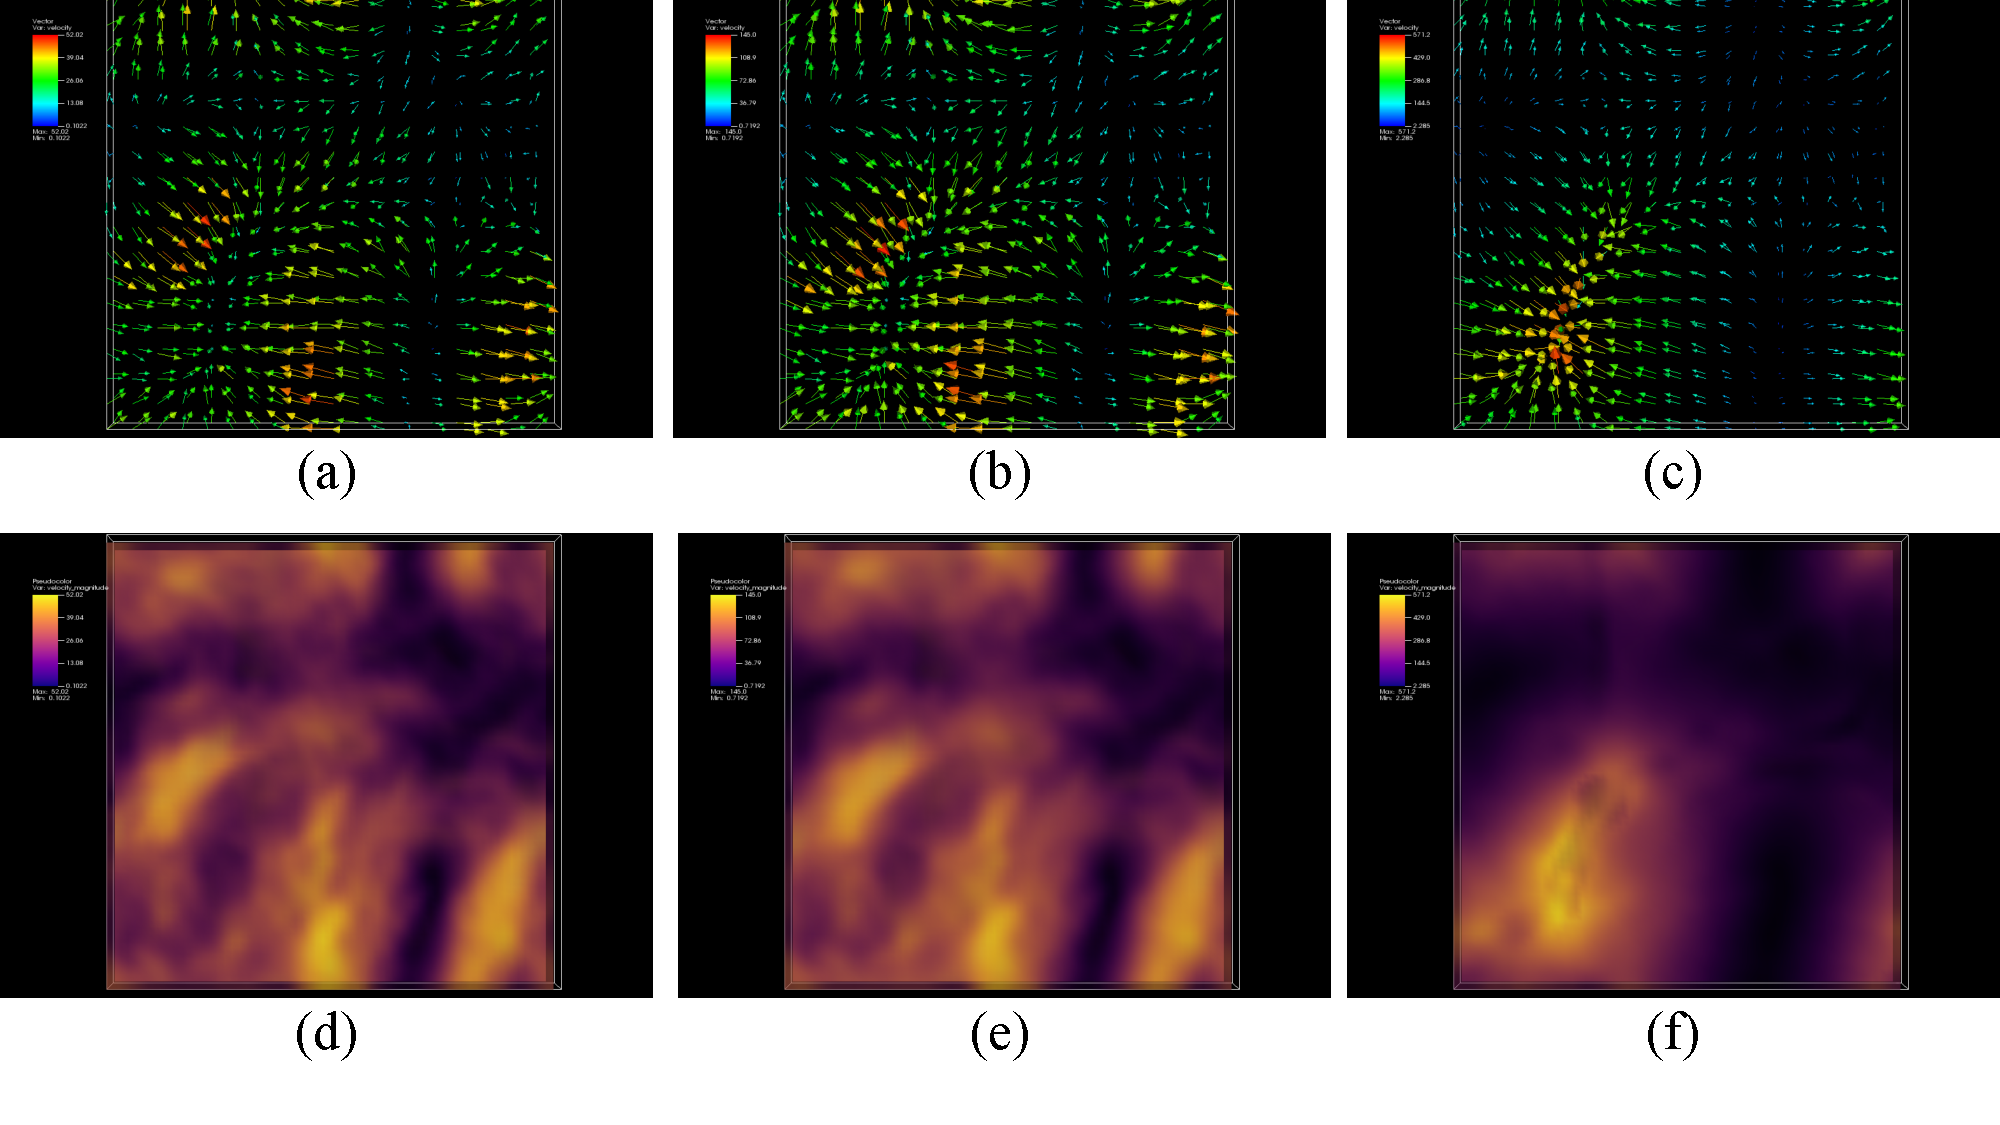
\includegraphics[width=1\linewidth, trim={0cm 1.1cm 0cm 0cm}, clip]{images/Nyx_vectorfields.pdf}
\vspace{-5mm}
\caption{Nyx vector field visualization: (a) and (d) show the vector field at time 0 and the maximum velocity magnitude is 52.02, (b) and (e) show the vector field at time 200 and the maximum velocity magnitude is 145.0, and finally, (c) and (f) show the vector field at time 400 and the maximum velocity is 571.2.}
\label{fig:vectorfield_nyx}
\vspace{-3mm}
\end{figure}




\begin{figure*}
\begin{minipage}[t]{0.33\linewidth}%
\begin{framed}
\setcounter{subfigure}{0}
\begin{minipage}[t]{0.49\textwidth}%
\centering
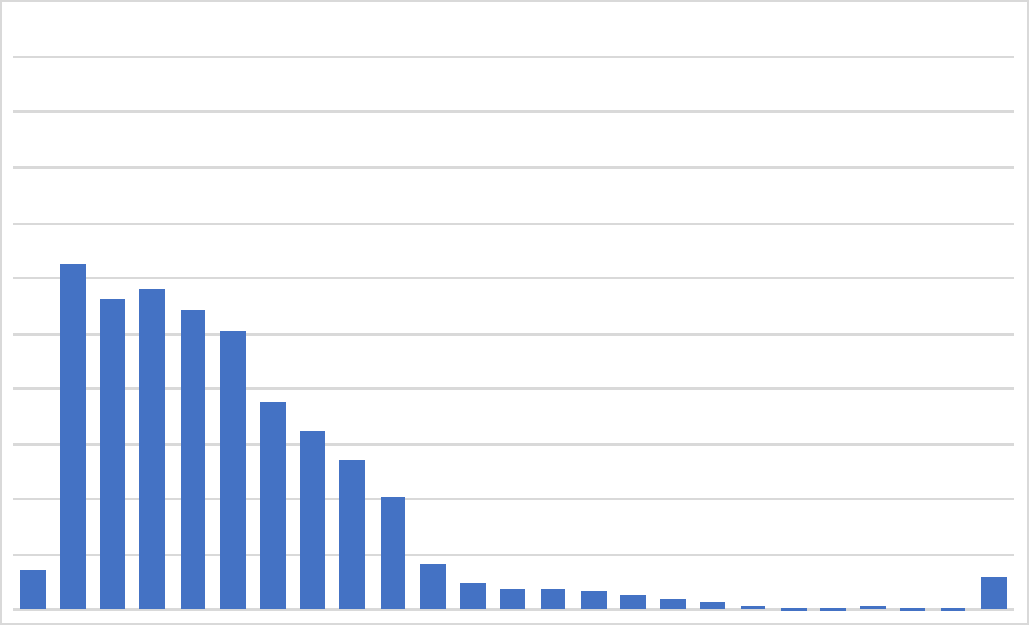
\includegraphics[width=0.95\textwidth]{results/sw4/Eul1_AvgL2.pdf}%
\vspace{-3mm}
\captionof{subfigure}{\footnotesize{Eul 250 Avg$_{L2}$}}
\end{minipage}%
\hfill
\begin{minipage}[t]{0.49\textwidth}%
\centering
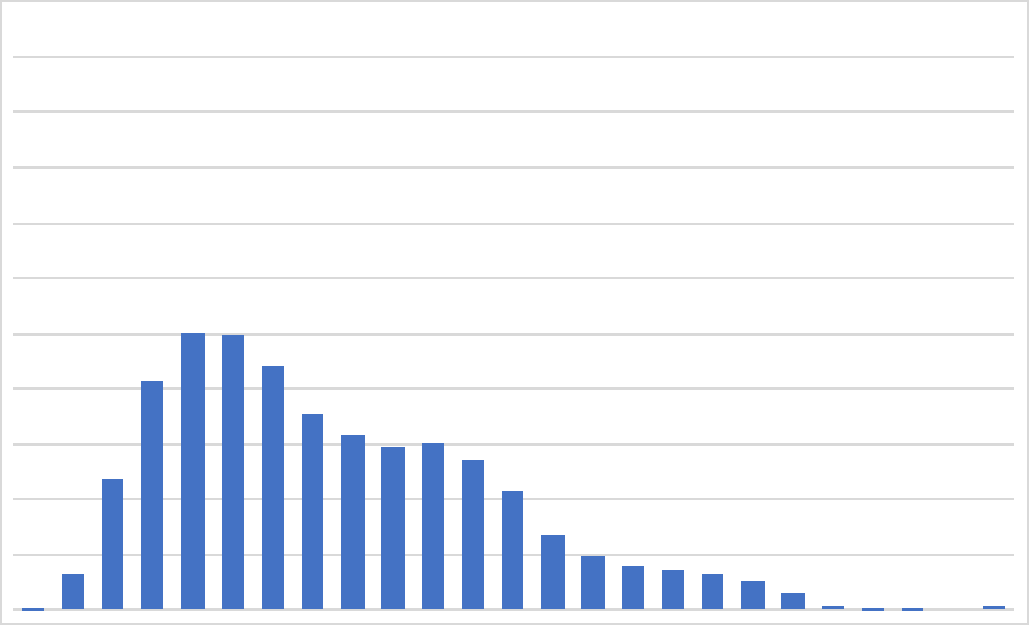
\includegraphics[width=0.95\linewidth]{results/sw4/Eul2_AvgL2.pdf}
\vspace{-3mm}
\captionof{subfigure}{\footnotesize{Eul 500 Avg$_{L2}$}} 
\end{minipage}
\begin{minipage}[t]{0.49\textwidth}%
\centering
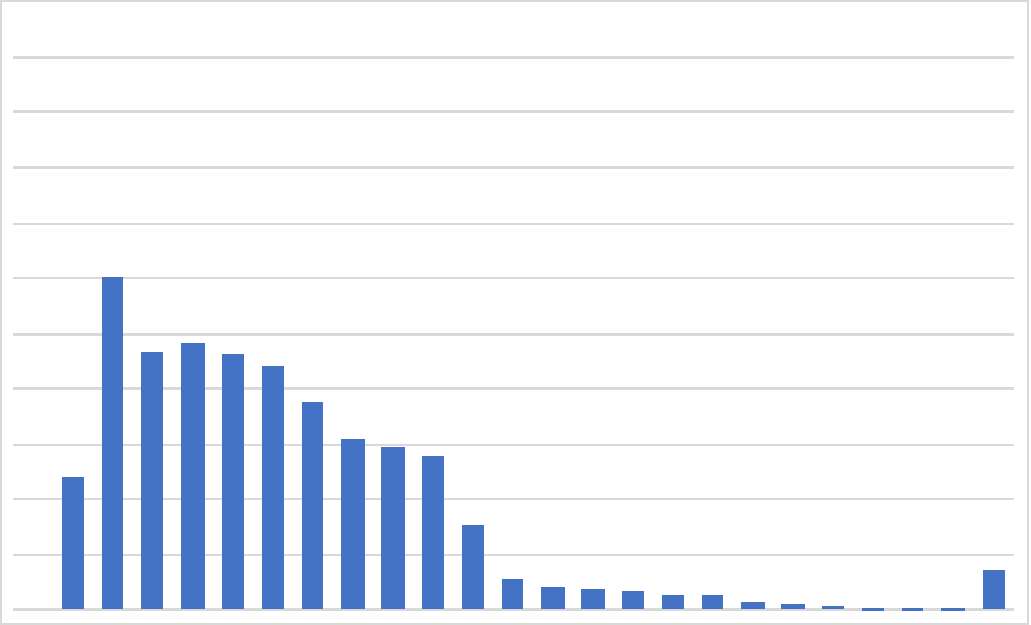
\includegraphics[width=0.95\textwidth]{results/sw4/Eul1_Max.pdf}%
\vspace{-3mm}
\captionof{subfigure}{\footnotesize{Eul 250 Max$_{L2}$}}
\end{minipage}%
\hfill
\begin{minipage}[t]{0.49\textwidth}%
\centering
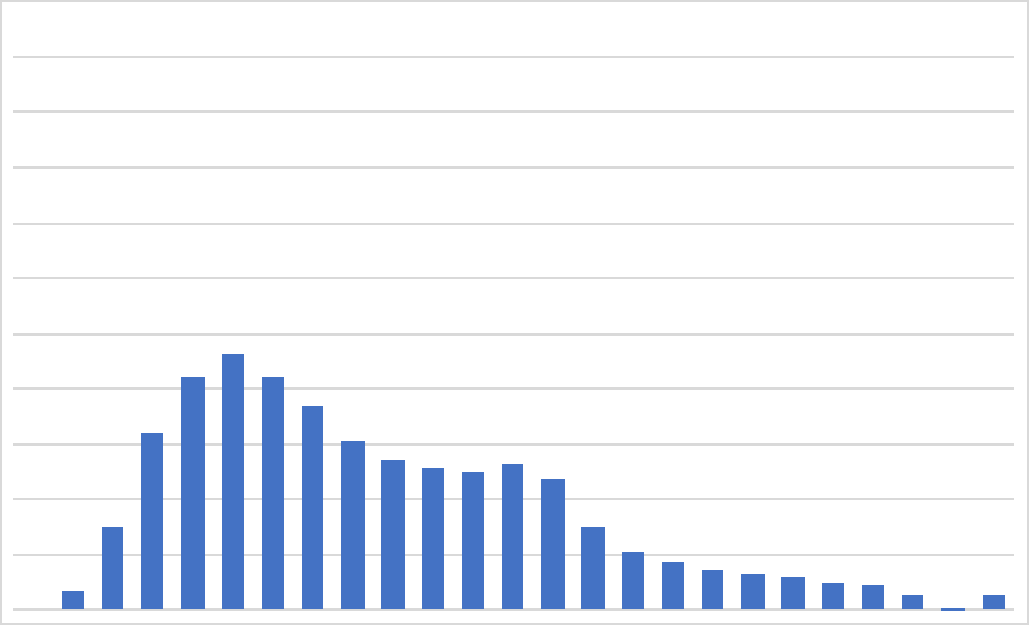
\includegraphics[width=0.95\linewidth]{results/sw4/Eul2_Max.pdf}
\vspace{-3mm}
\captionof{subfigure}{\footnotesize{Eul 500 Max$_{L2}$}} 
\end{minipage}
\begin{minipage}[t]{0.49\textwidth}%
\centering
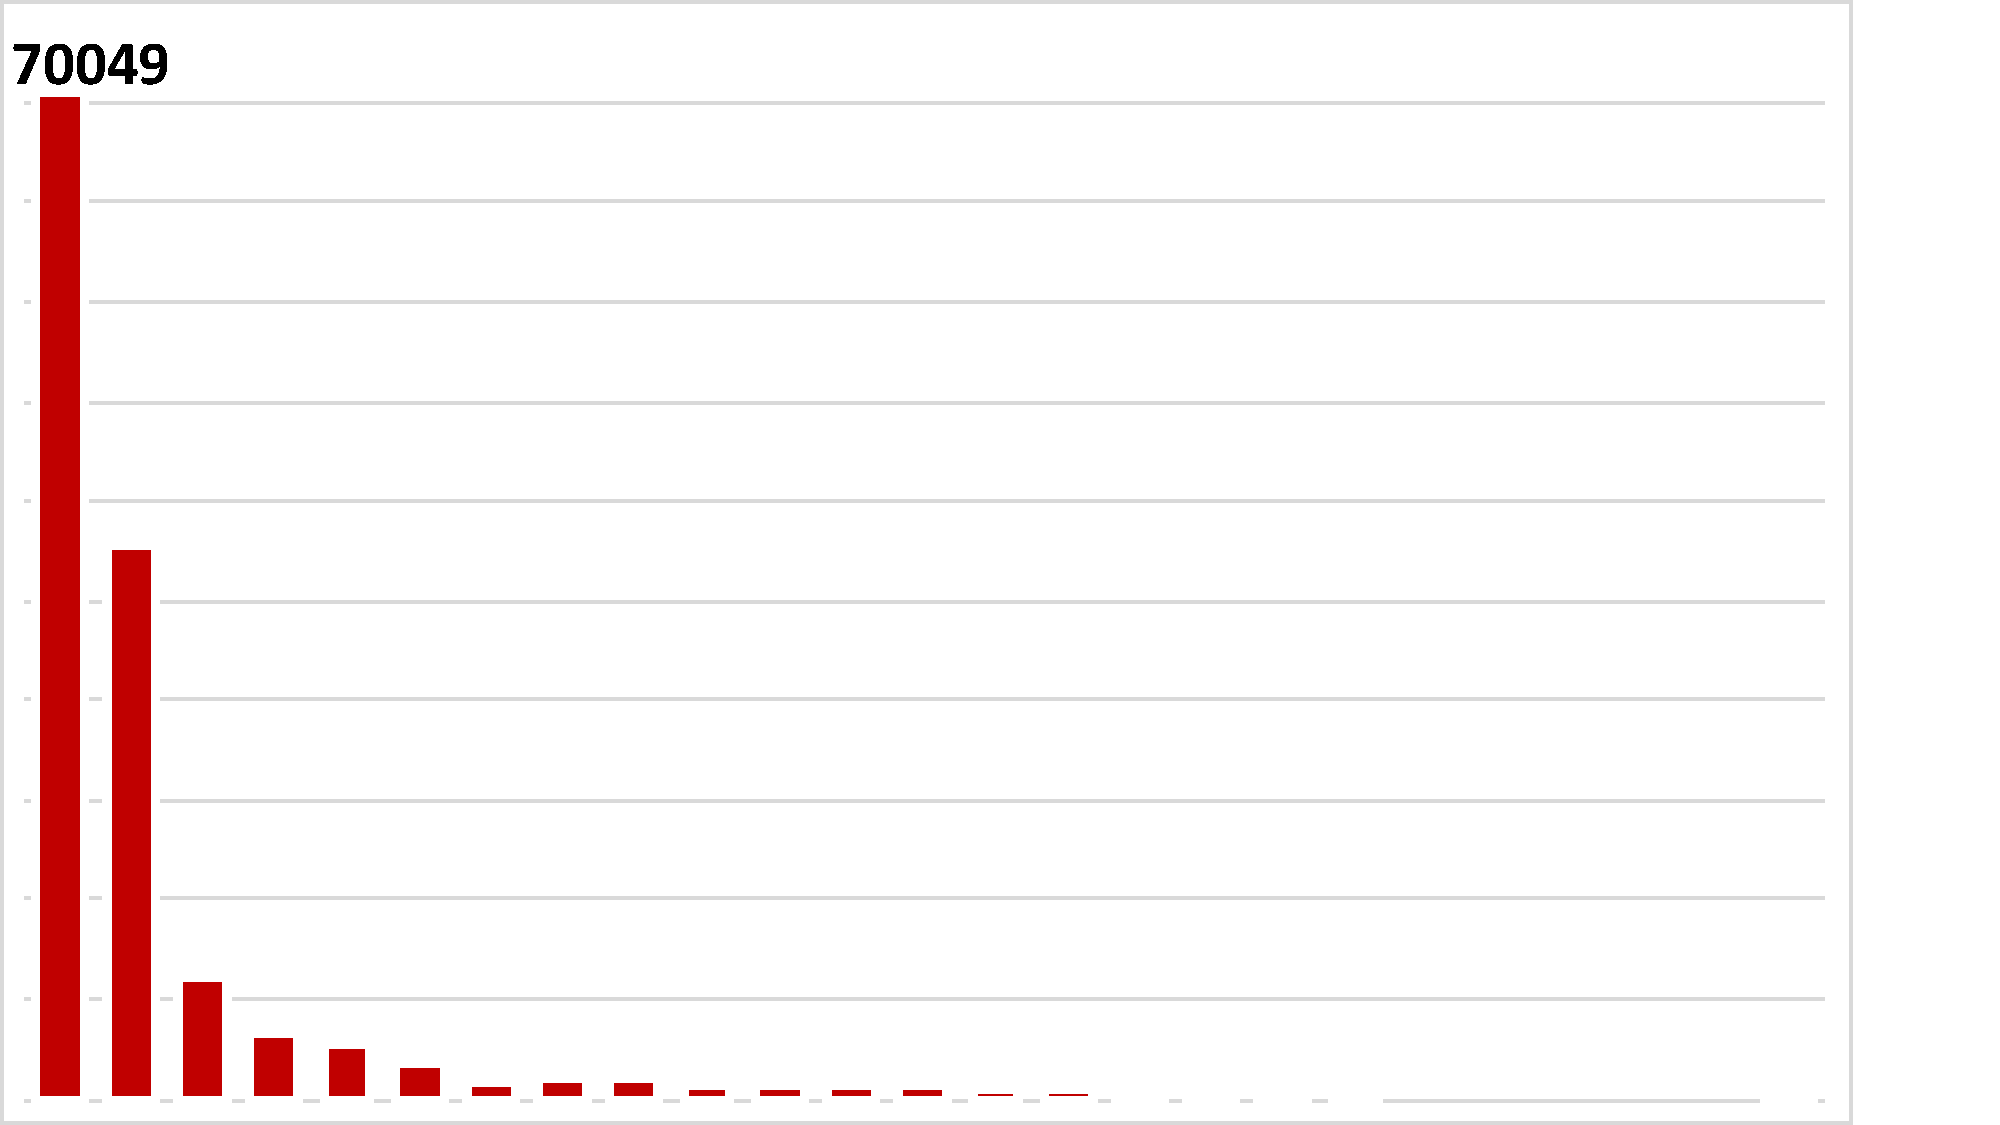
\includegraphics[width=0.95\linewidth, trim={0cm 0cm 2.5cm 0cm}, clip]{results/sw4/Lag3_AvgL2.pdf}
\vspace{-3mm}
\captionof{subfigure}{\footnotesize{Lag 250 1:27 Avg$_{L2}$}}
\end{minipage}%
\hfill
\begin{minipage}[t]{0.49\textwidth}%
\centering
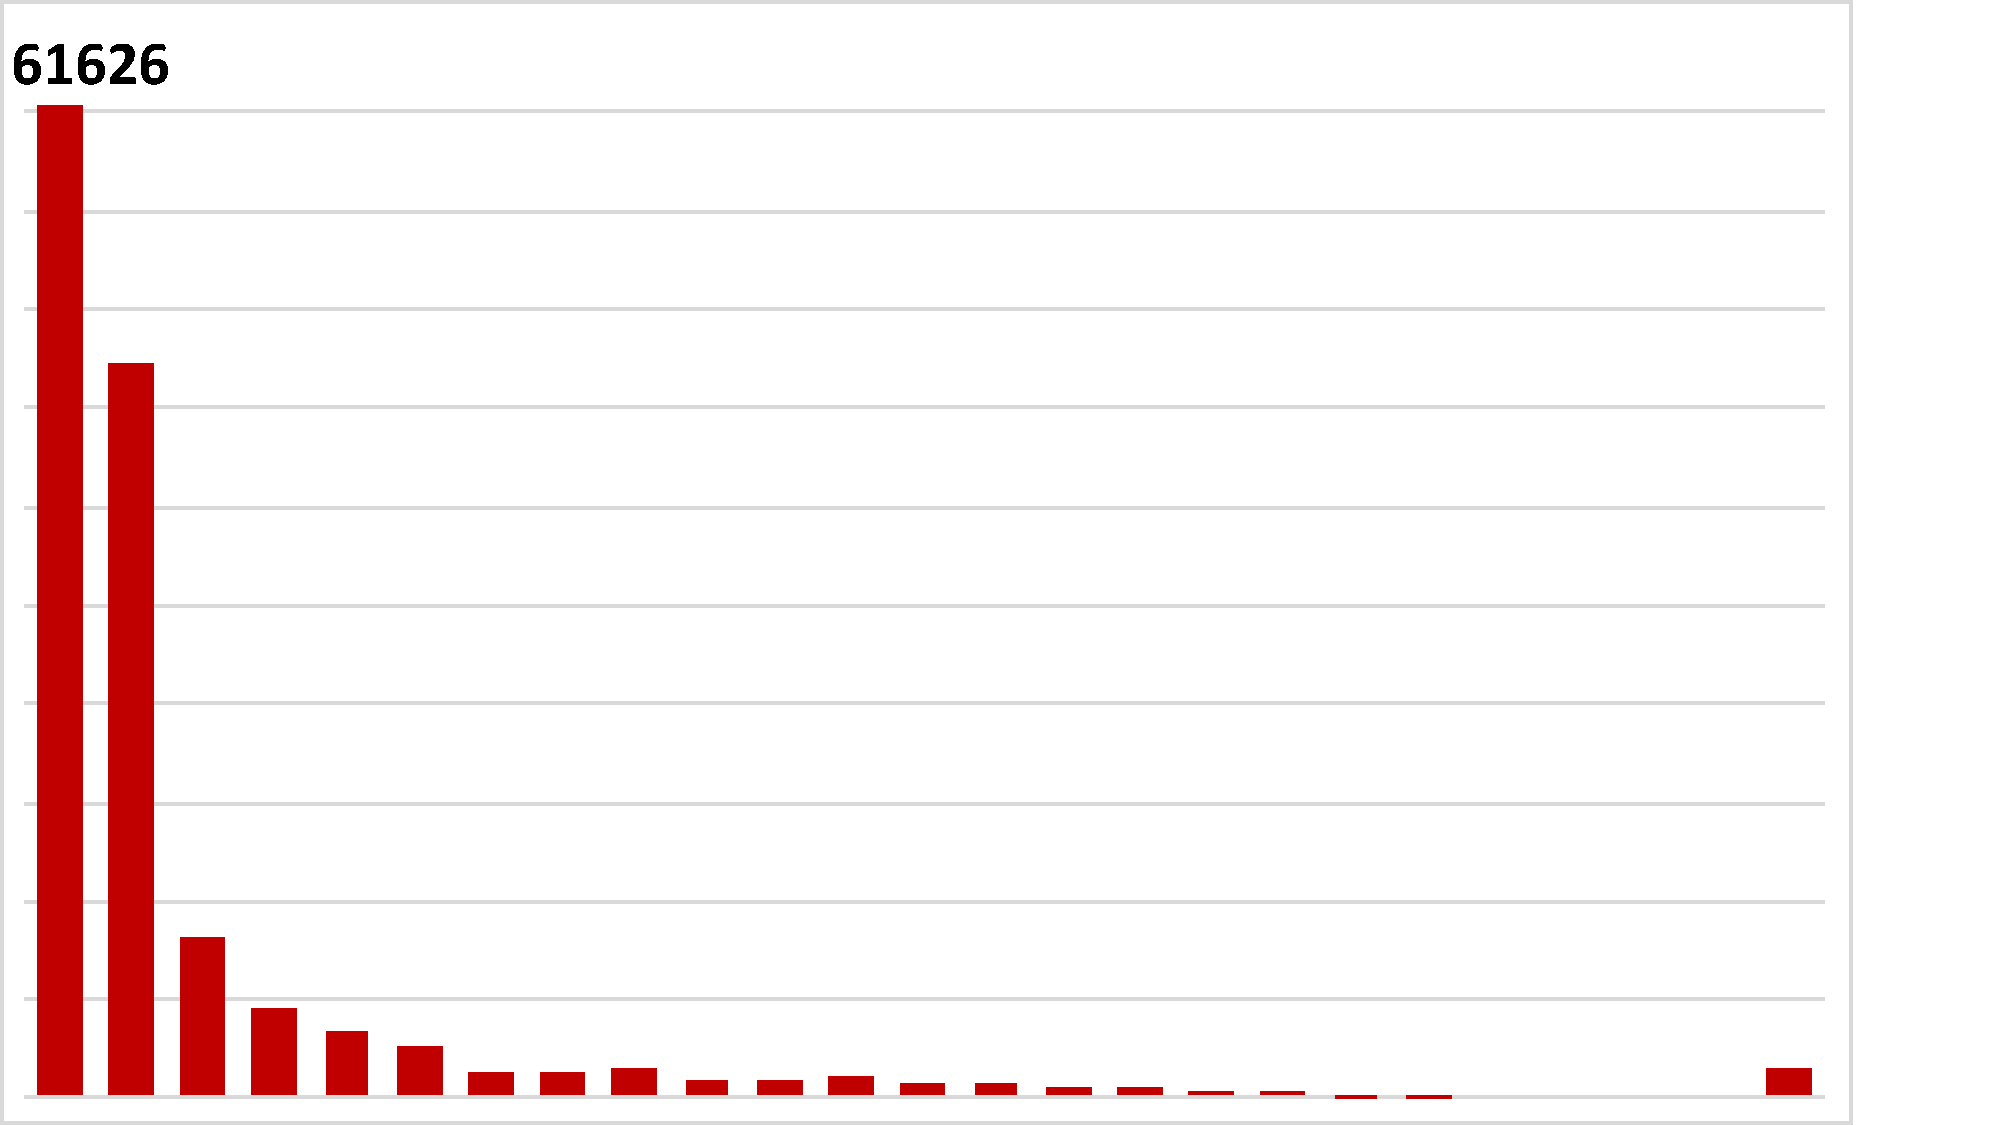
\includegraphics[width=0.95\linewidth, trim={0cm 0cm 2.5cm 0cm}, clip]{results/sw4/Lag4_AvgL2.pdf}
\vspace{-3mm}
\captionof{subfigure}{\footnotesize{Lag 250 1:64 Avg$_{L2}$}} 
\end{minipage}
\begin{minipage}[t]{0.49\textwidth}%
\centering
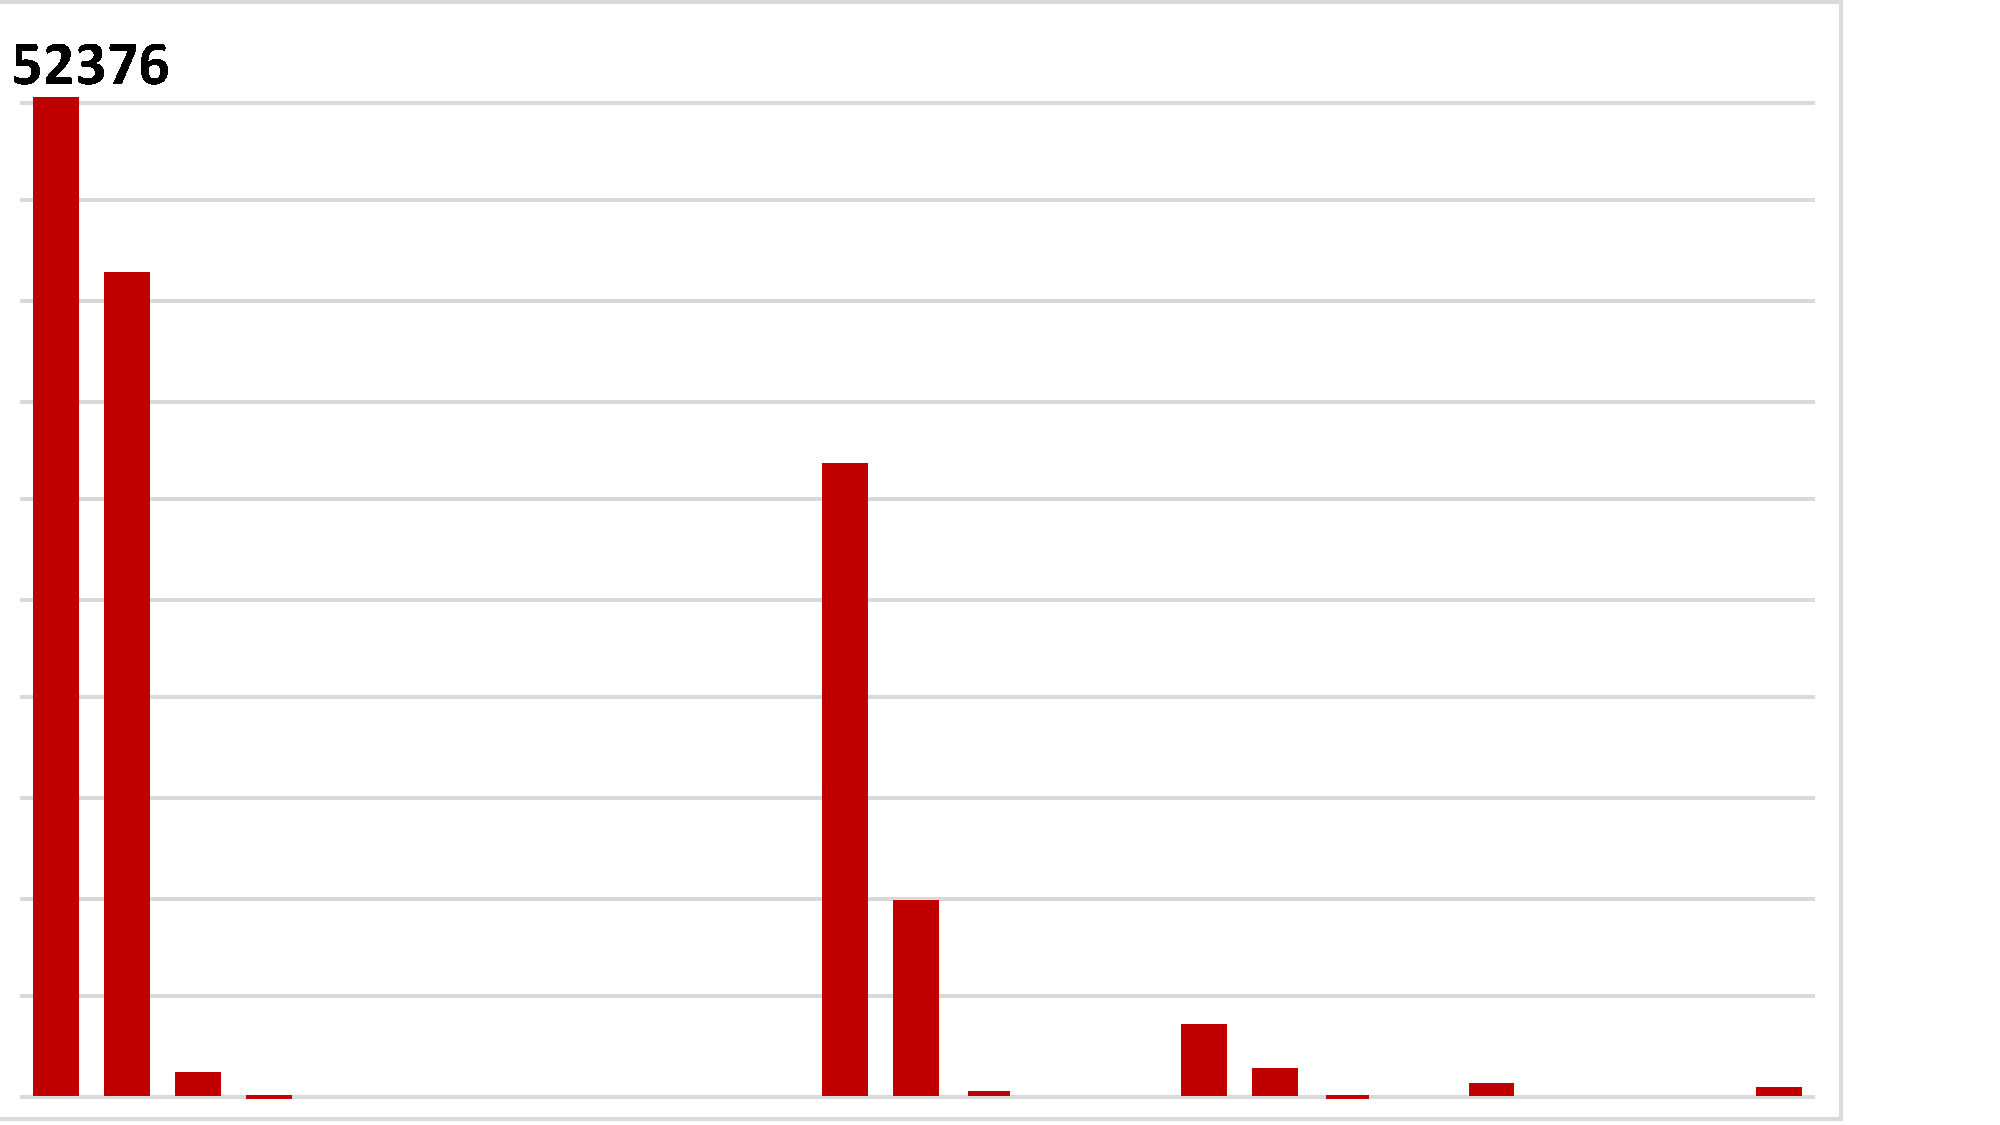
\includegraphics[width=0.95\linewidth, trim={0cm 0cm 2.5cm 0cm}, clip]{results/sw4/Lag3_Max.pdf}
\vspace{-3mm}
\captionof{subfigure}{\footnotesize{Lag 250 1:27 Max$_{L2}$}}
\end{minipage}%
\hfill
\begin{minipage}[t]{0.49\textwidth}%
\centering
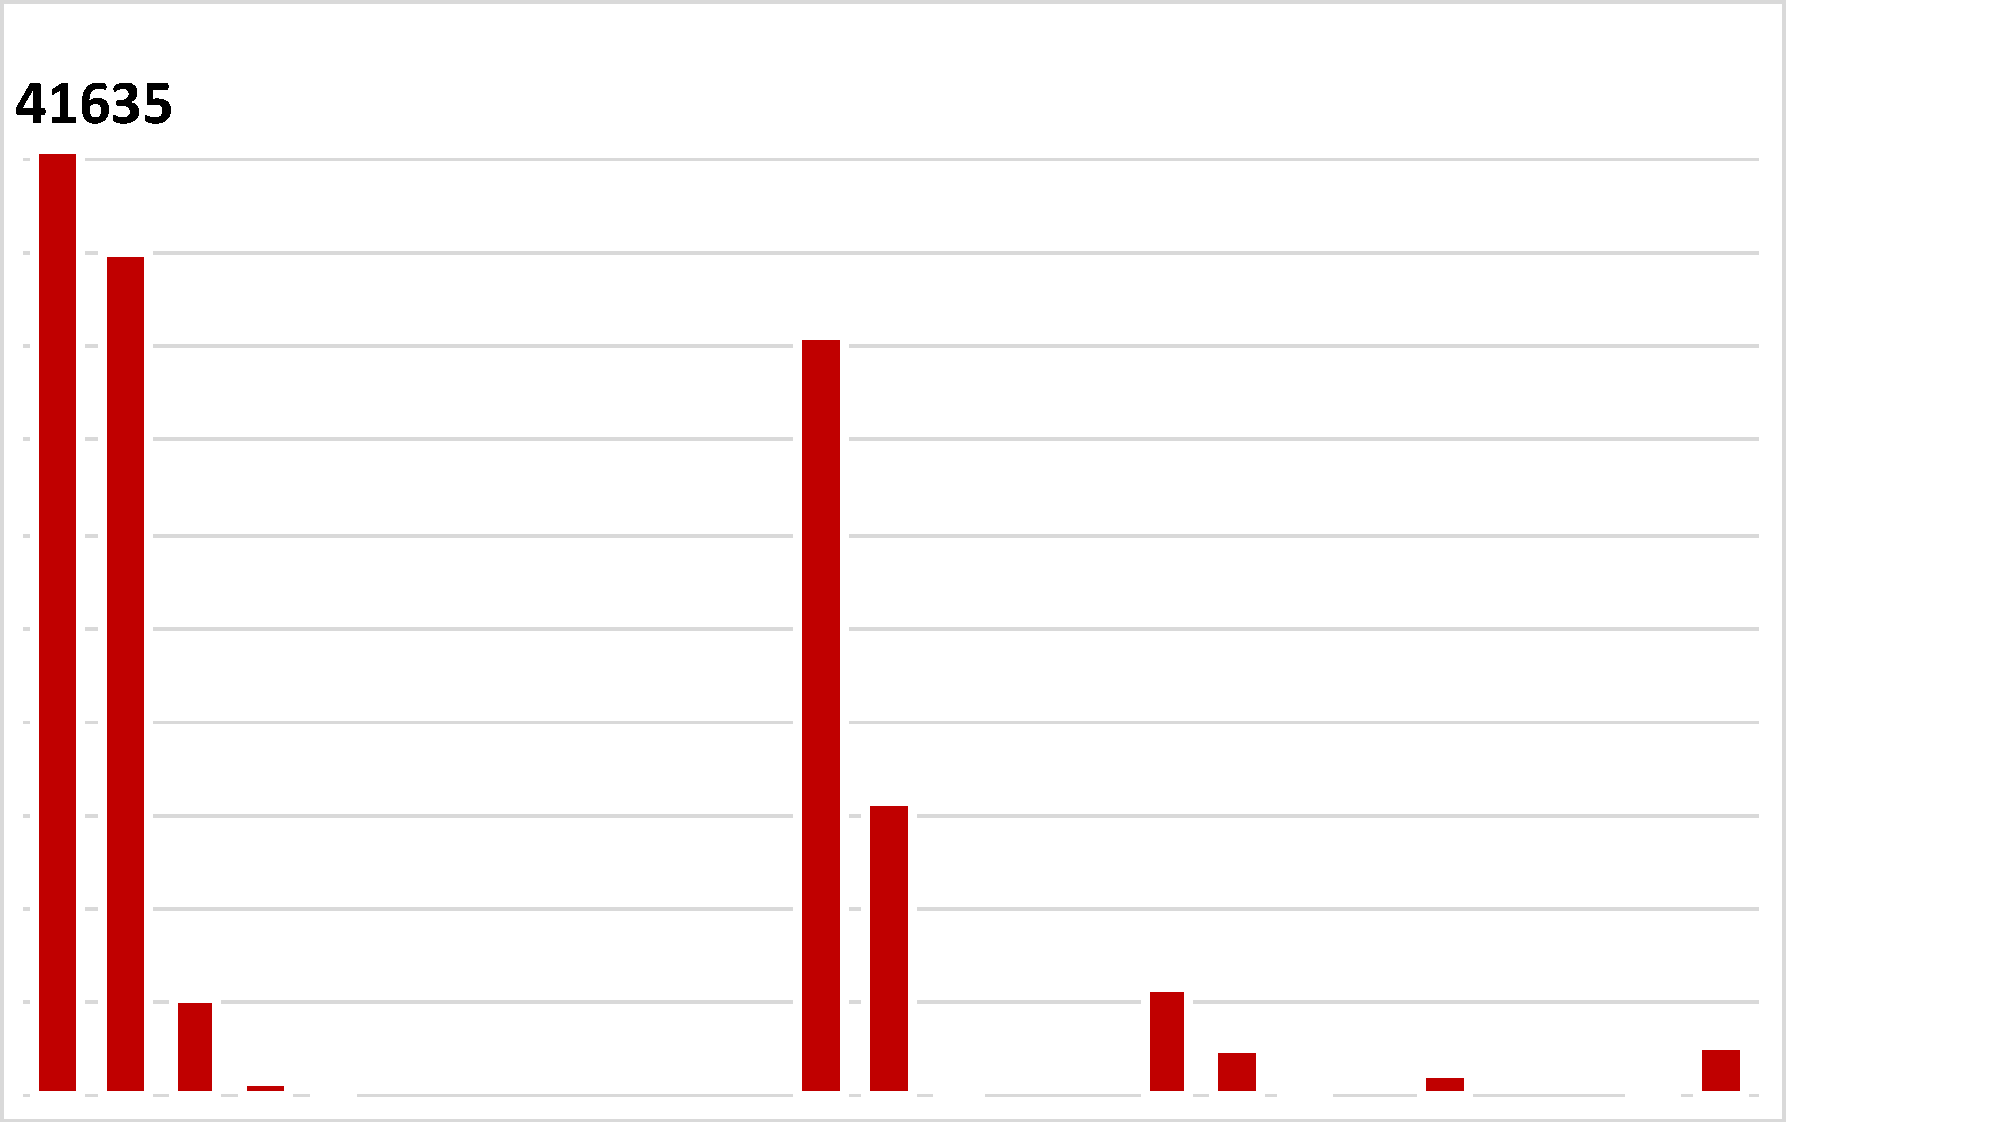
\includegraphics[width=0.95\linewidth, trim={0cm 0cm 2.5cm 0cm}, clip]{results/sw4/Lag4_Max.pdf}
\vspace{-3mm}
\captionof{subfigure}{\footnotesize{Lag 250 1:64 Max$_{L2}$}} 
\end{minipage}
\end{framed}
\vspace{-2mm}
\captionof{figure}{\textbf{SW4} experiment histograms for 90,000 test particle interpolation errors. Each plot has 25 bins, Eulerian bins range from $<$0.6 to $>$15, Lagrangian bins range from 0 to $>$0.2, with bar height encoding number of particles. Horizontal grid lines mark increments of 2,000.}
\label{fig:sw4_histograms}
\end{minipage}% End of SW4
%%%%%%%%%%%%%%%%%%%%%%%%%%%%%%%%%%%
\setcounter{subfigure}{0}
\hfill
\begin{minipage}[t]{0.66\linewidth}%
\begin{framed}
\begin{minipage}[t]{0.24\textwidth}%
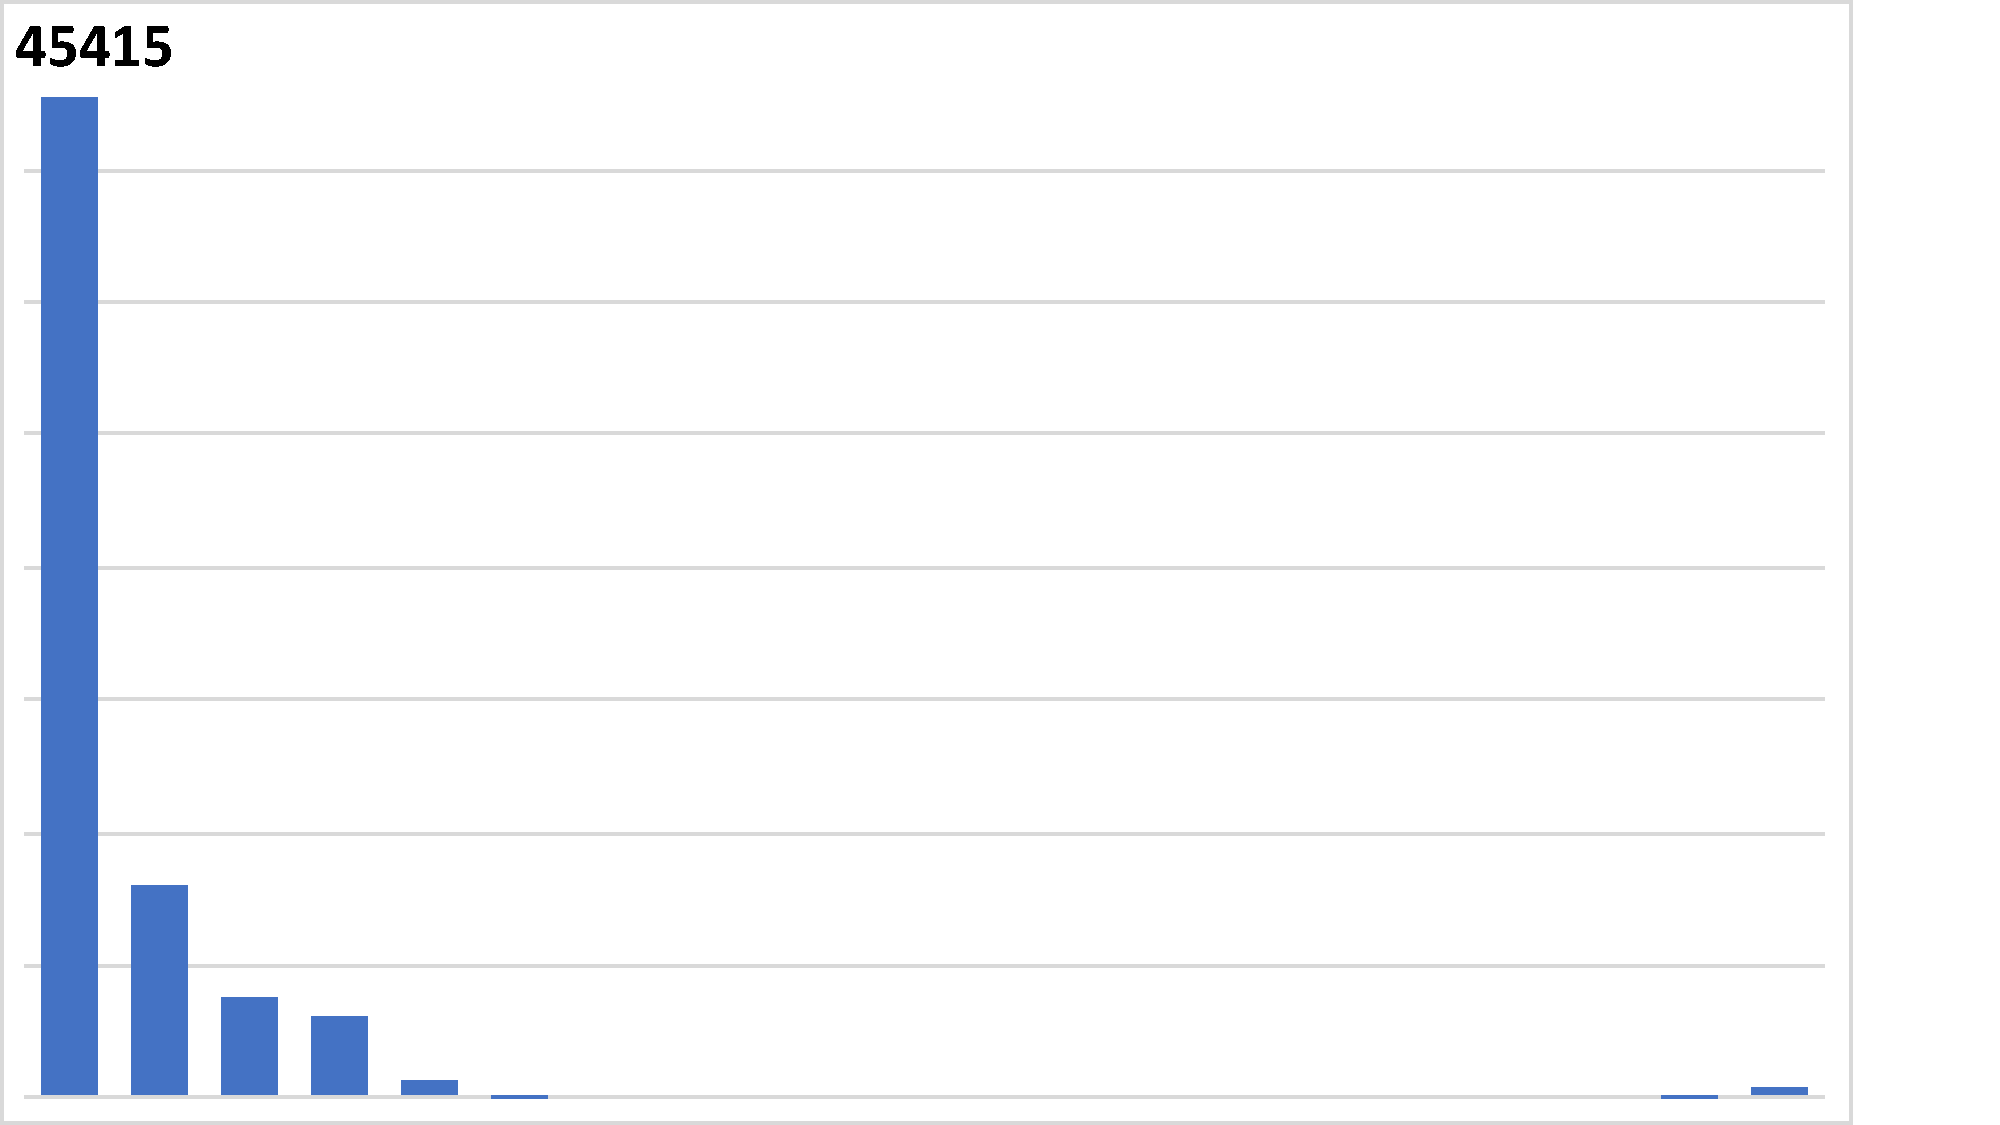
\includegraphics[width=0.95\linewidth, trim={0cm 0cm 2.5cm 0cm}, clip]{results/nyx/Eul25_AvgL2.pdf}
\vspace{-2mm}
\captionof{subfigure}{Eul 25 Avg$_{L2}$}
\end{minipage}%
\hfill
\begin{minipage}[t]{0.24\textwidth}%
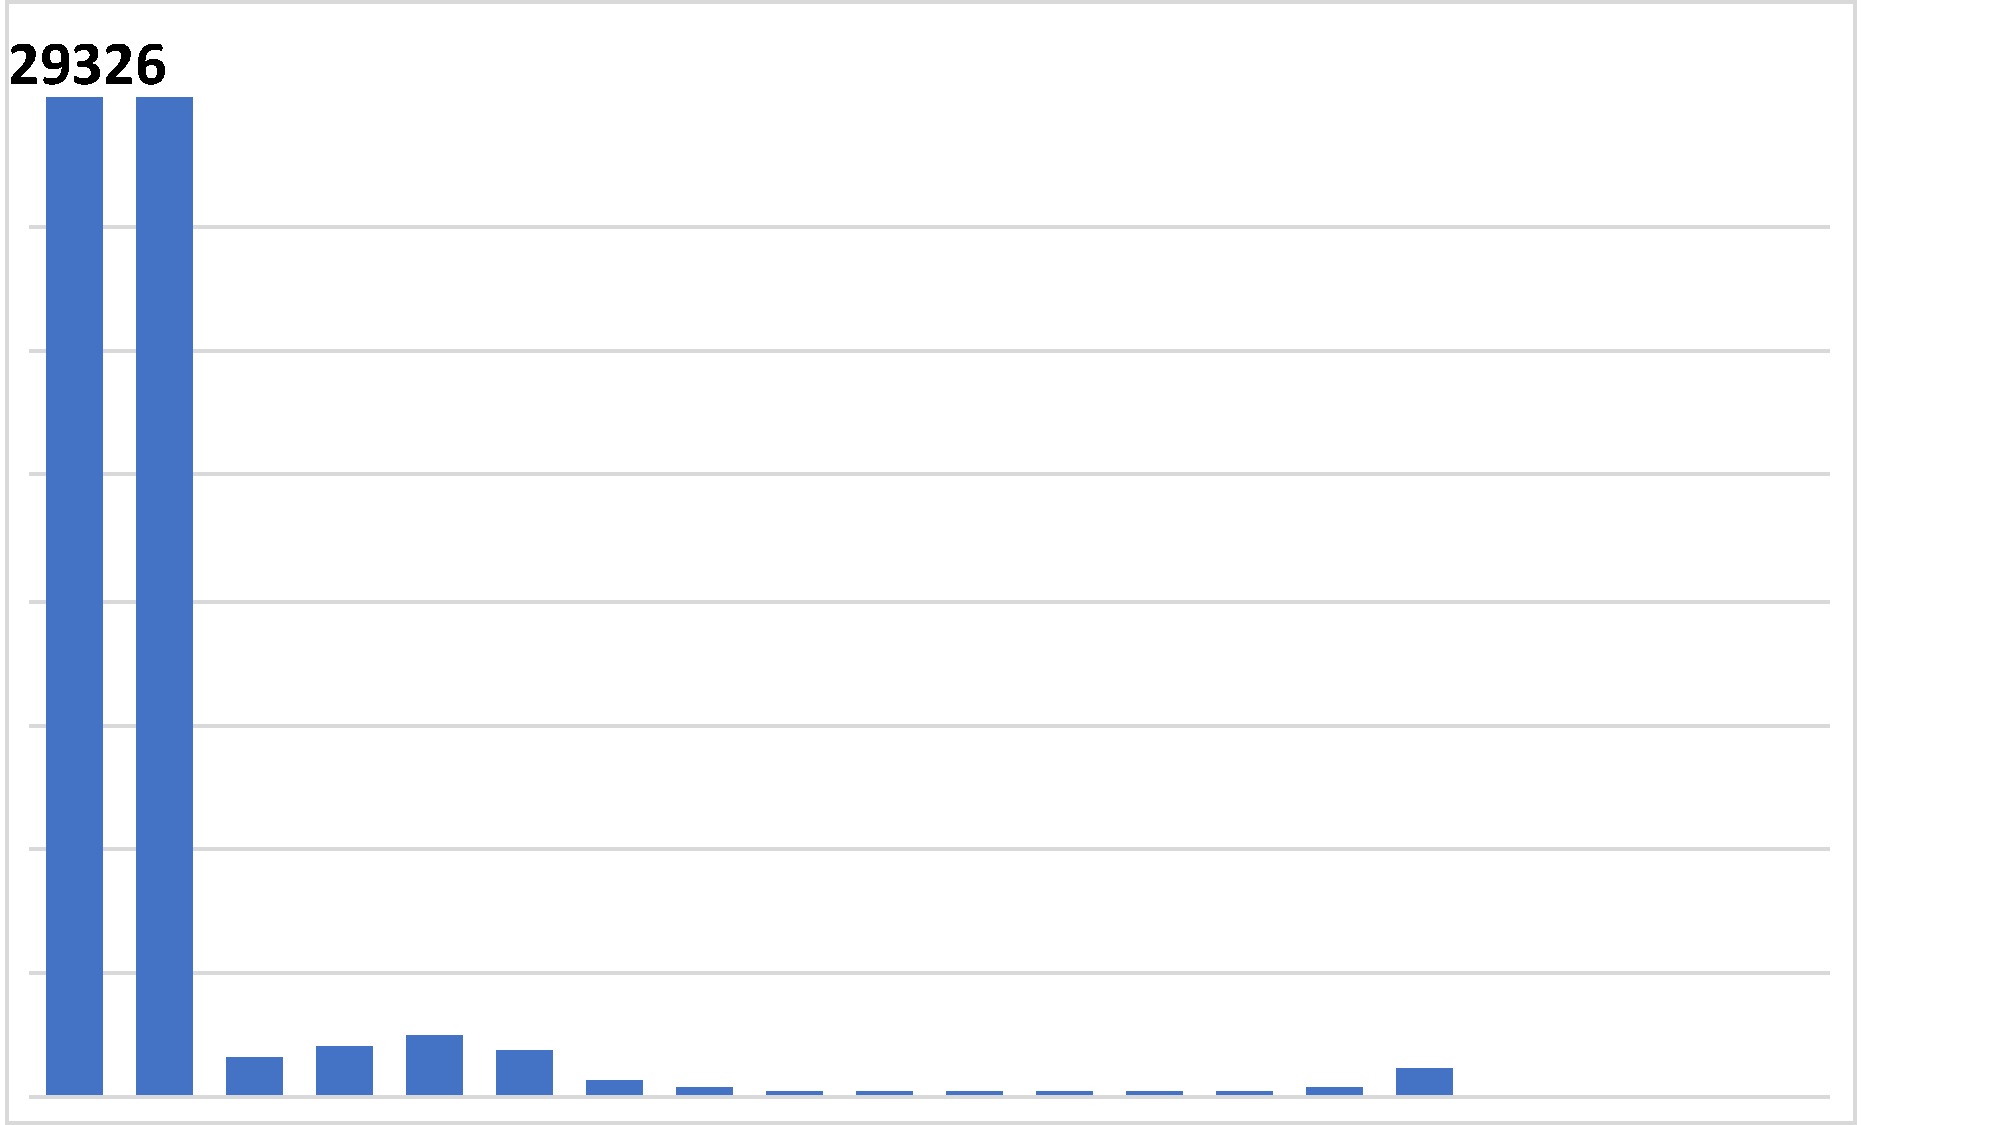
\includegraphics[width=0.95\linewidth, trim={0cm 0cm 2.5cm 0cm}, clip]{results/nyx/Eul50_AvgL2.pdf}
\vspace{-2mm}
\captionof{subfigure}{Eul 50 Avg$_{L2}$}
\end{minipage}
\begin{minipage}[t]{0.24\textwidth}%
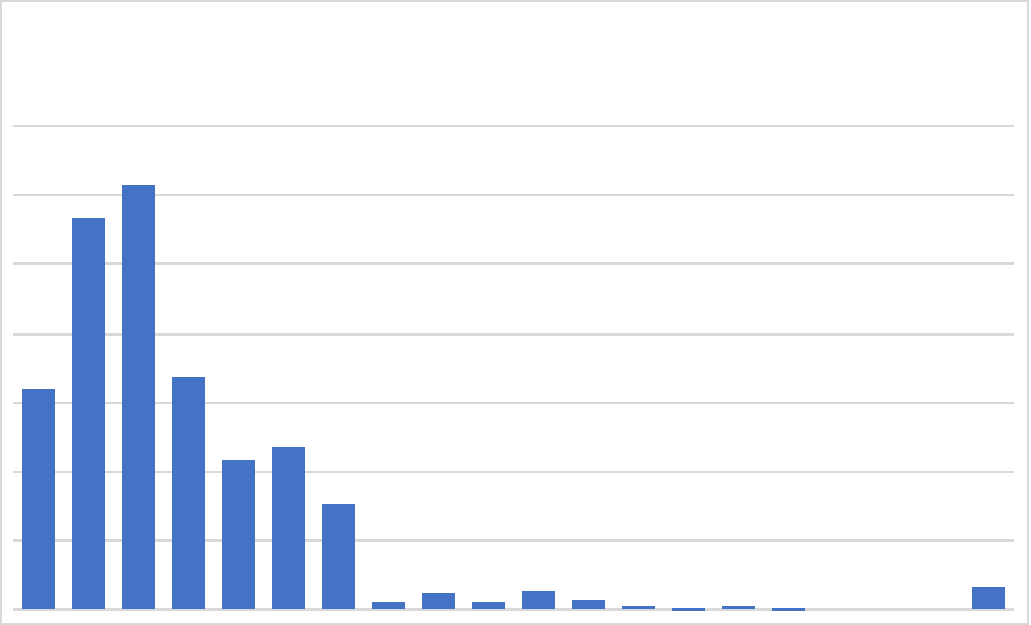
\includegraphics[width=0.95\linewidth]{results/nyx/Eul100_AvgL2.pdf}
\vspace{-2mm}
\captionof{subfigure}{Eul 100 Avg$_{L2}$}
\end{minipage}%
\hfill
\begin{minipage}[t]{0.24\textwidth}%
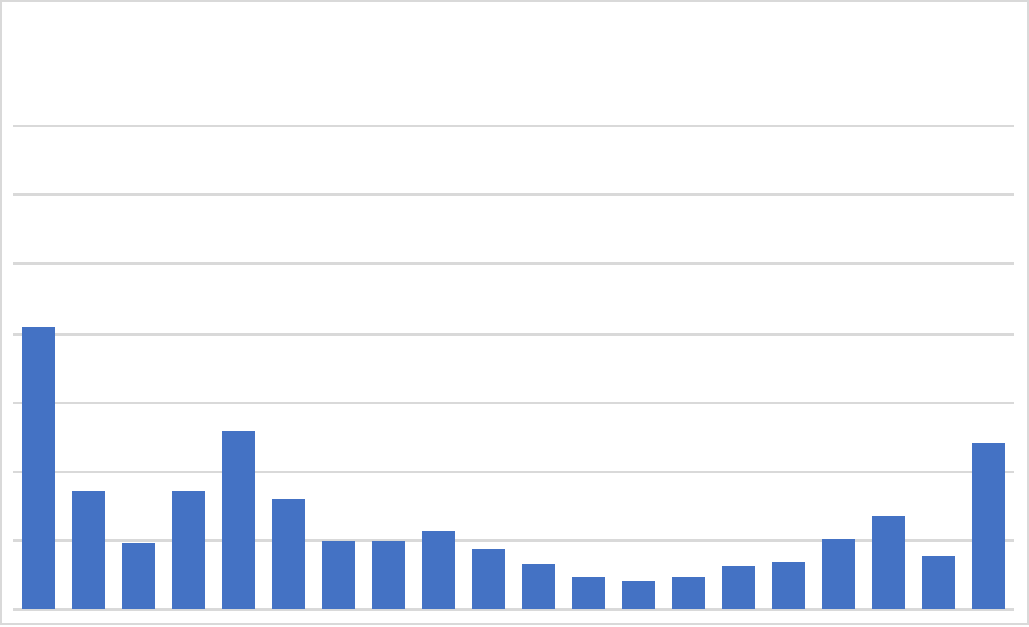
\includegraphics[width=0.95\linewidth]{results/nyx/Eul200_AvgL2.pdf}
\vspace{-2mm}
\captionof{subfigure}{Eul 200 Avg$_{L2}$}
\end{minipage}
\begin{minipage}[t]{0.24\textwidth}%
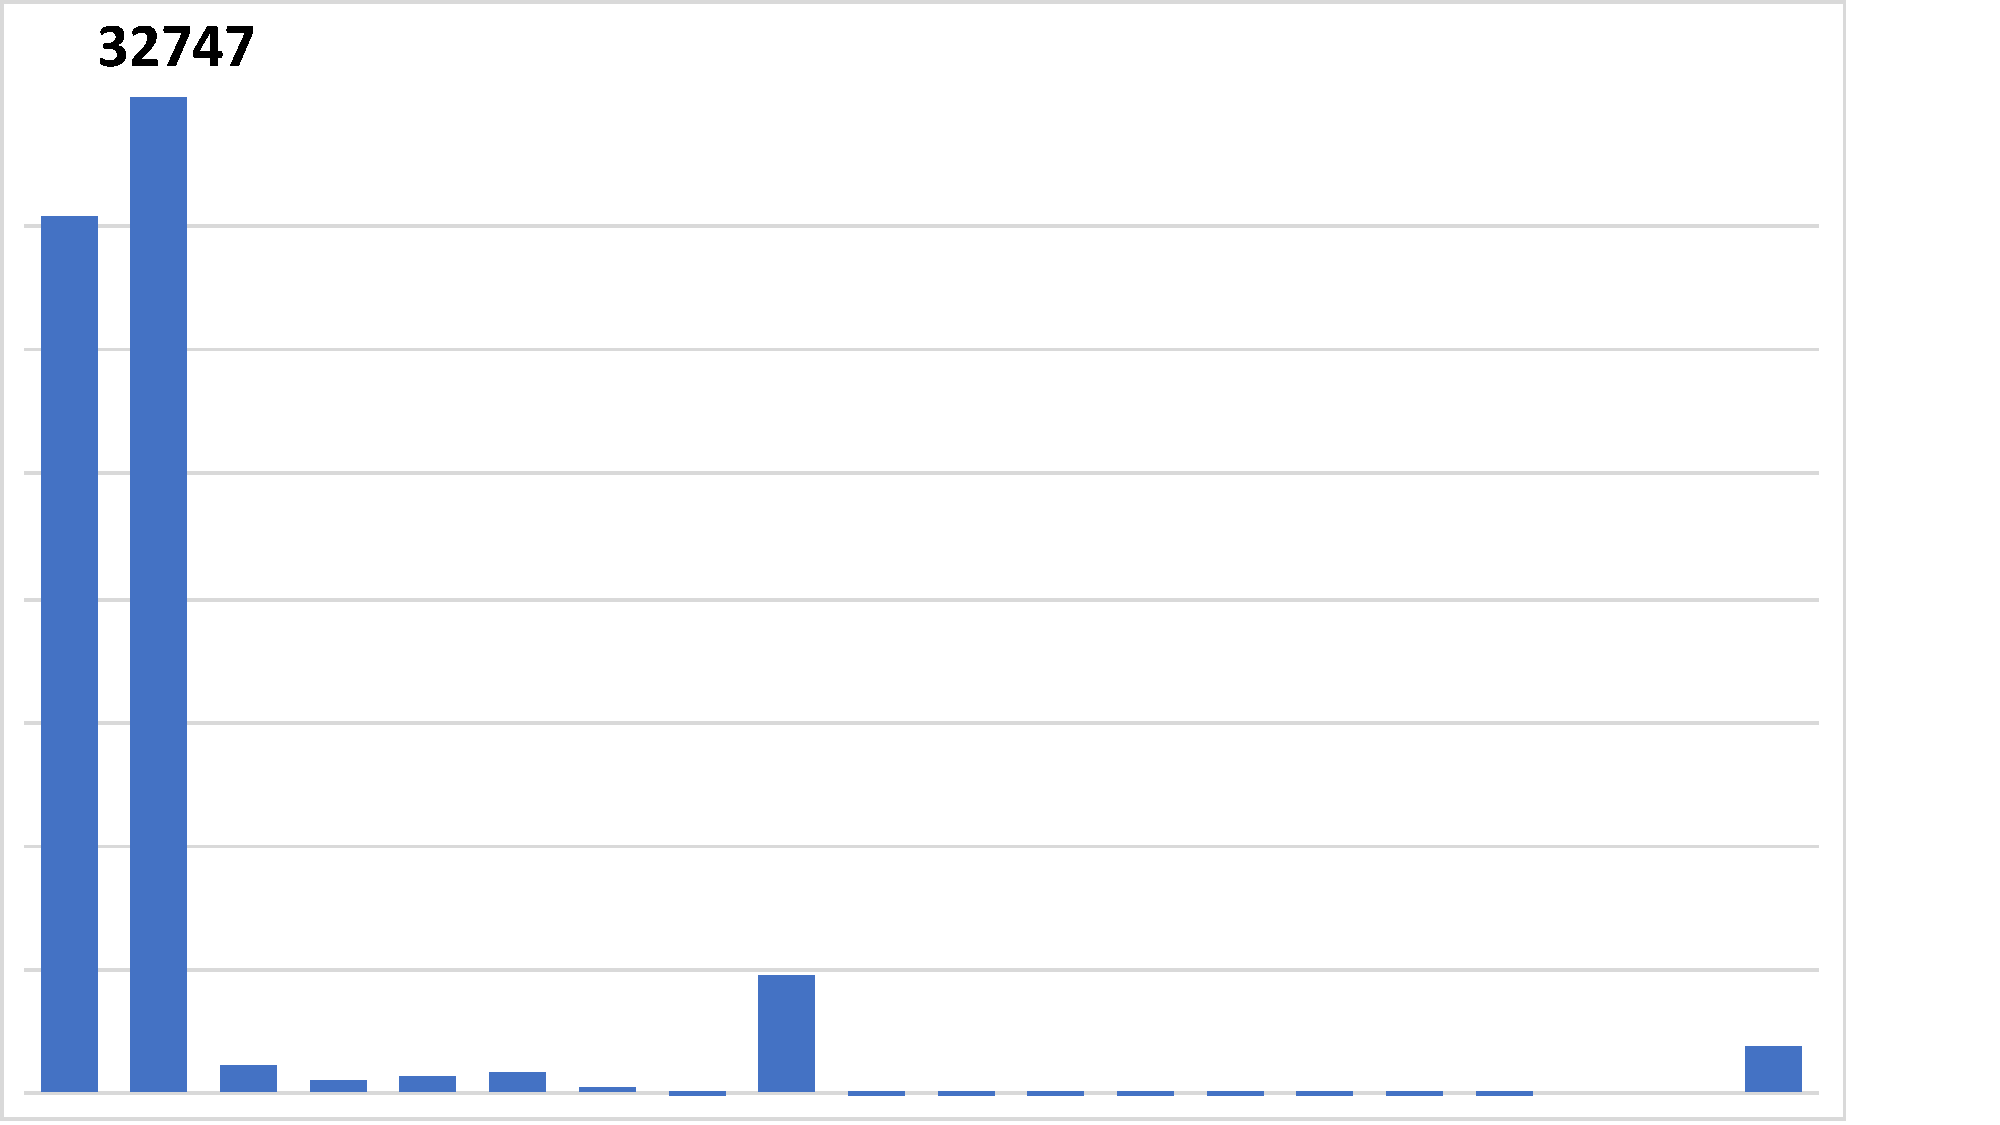
\includegraphics[width=0.95\linewidth, trim={0cm 0cm 2.5cm 0cm}, clip]{results/nyx/Eul25_Max.pdf}
\vspace{-2mm}
\captionof{subfigure}{Eul 25 Max$_{L2}$}
\end{minipage}%
\hfill
\begin{minipage}[t]{0.24\textwidth}%
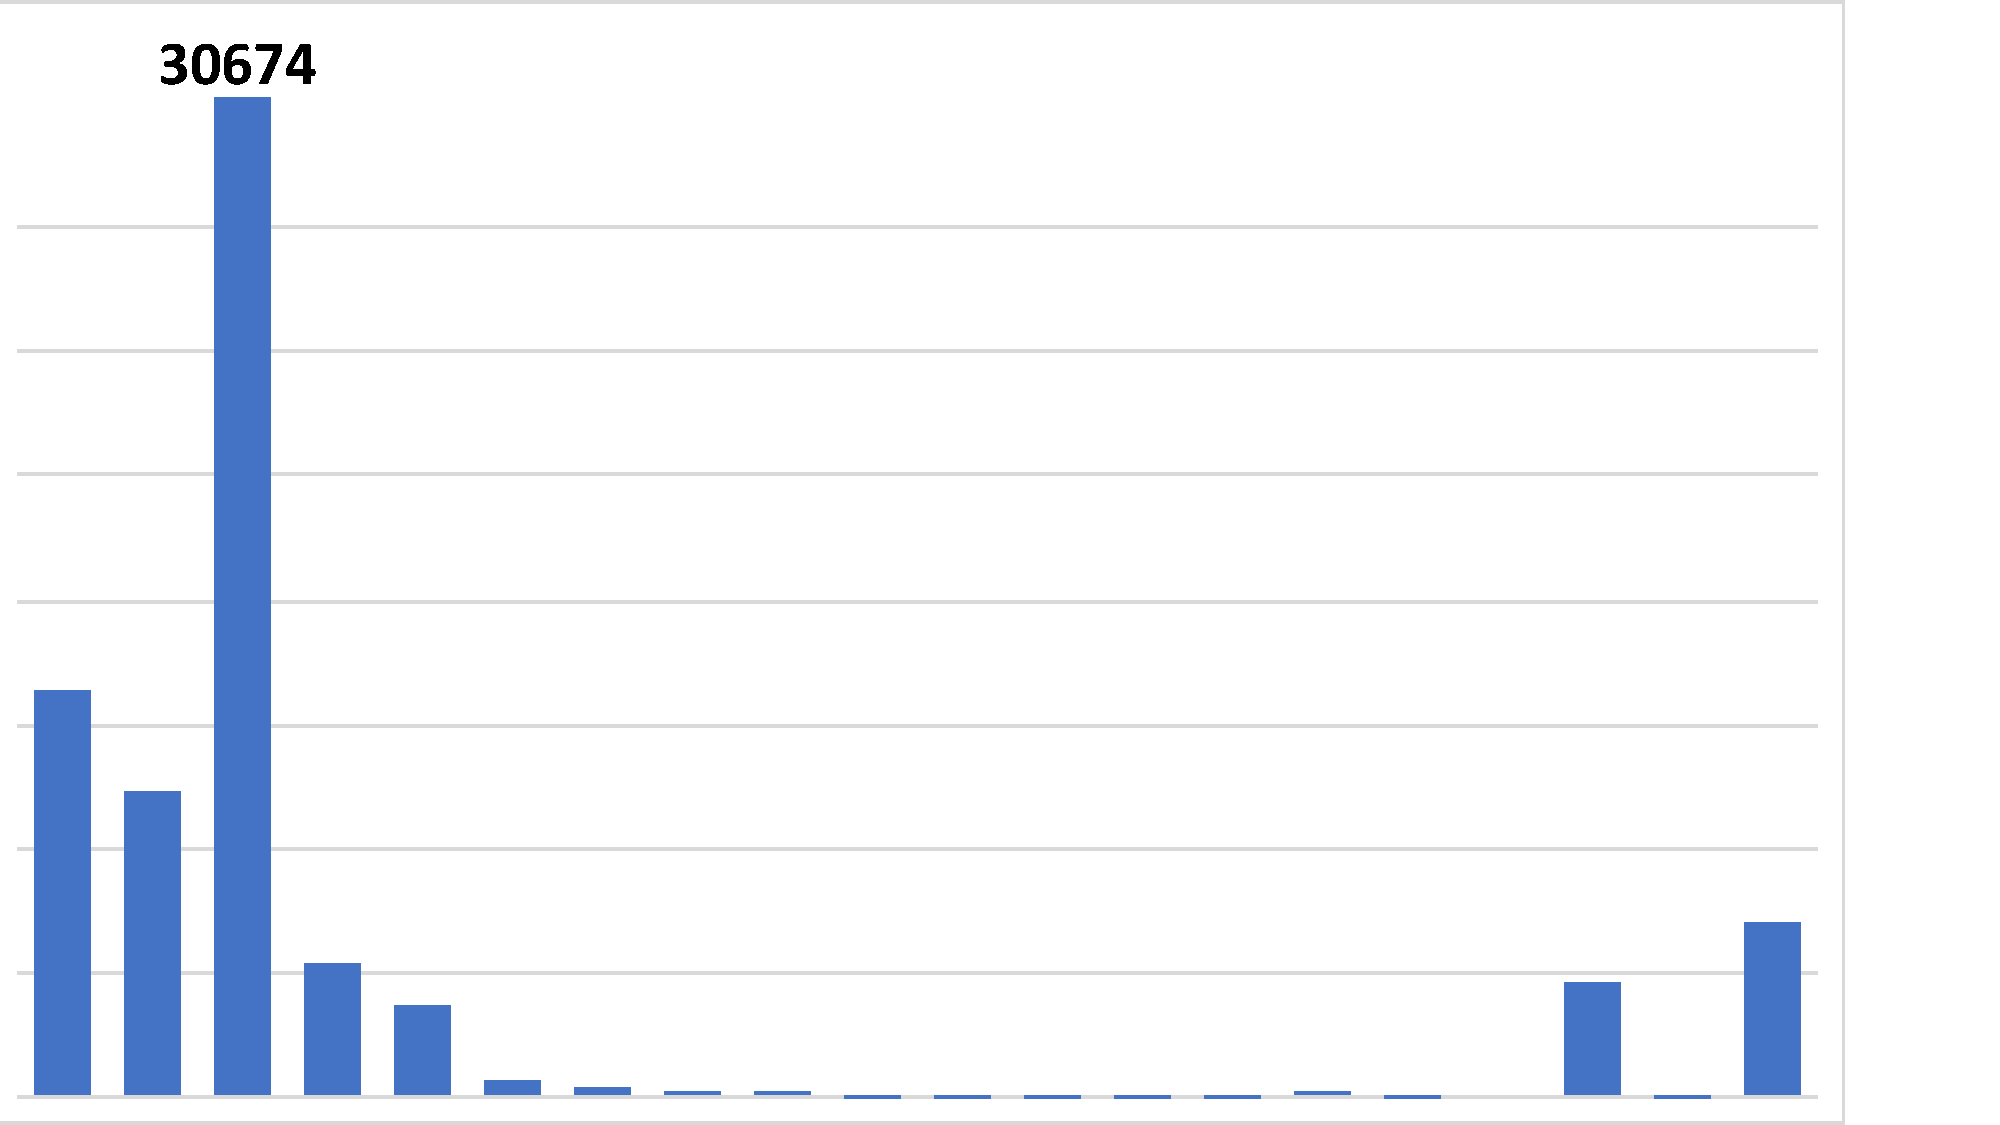
\includegraphics[width=0.95\linewidth, trim={0cm 0cm 2.5cm 0cm}, clip]{results/nyx/Eul50_Max.pdf}
\vspace{-2mm}
\captionof{subfigure}{Eul 50 Max$_{L2}$}
\end{minipage}
\begin{minipage}[t]{0.24\textwidth}%
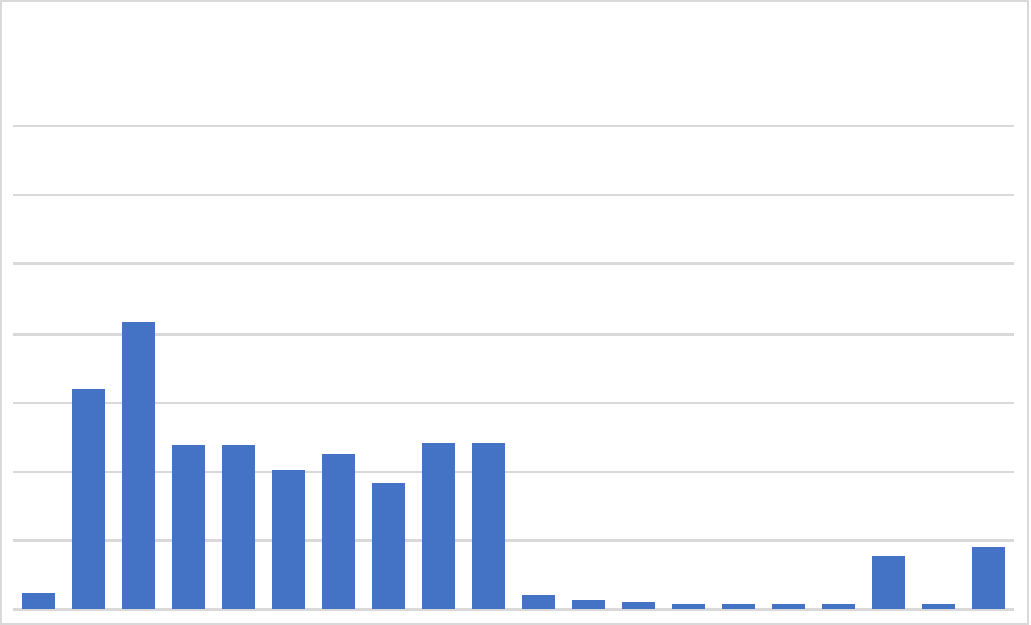
\includegraphics[width=0.95\linewidth]{results/nyx/Eul100_Max.pdf}
\vspace{-2mm}
\captionof{subfigure}{Eul 100 Max$_{L2}$}
\end{minipage}%
\hfill
\begin{minipage}[t]{0.24\textwidth}%
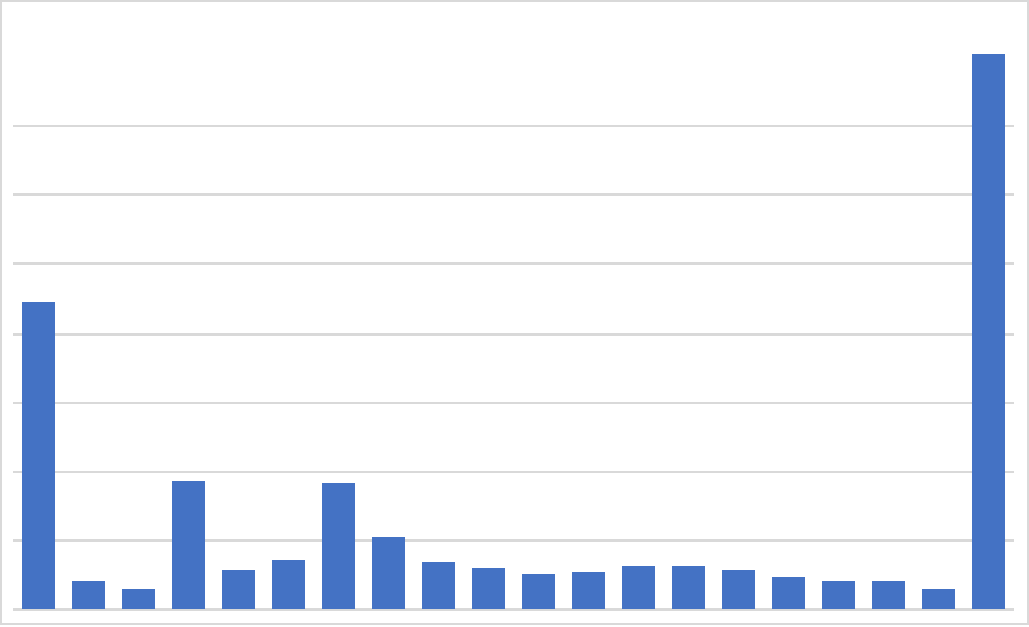
\includegraphics[width=0.95\linewidth]{results/nyx/Eul200_Max.pdf}
\vspace{-2mm}
\captionof{subfigure}{Eul 200 Max$_{L2}$}
\end{minipage}
%%%% Begin Nyx Lagrangian %%% 
\begin{minipage}[t]{0.24\textwidth}%
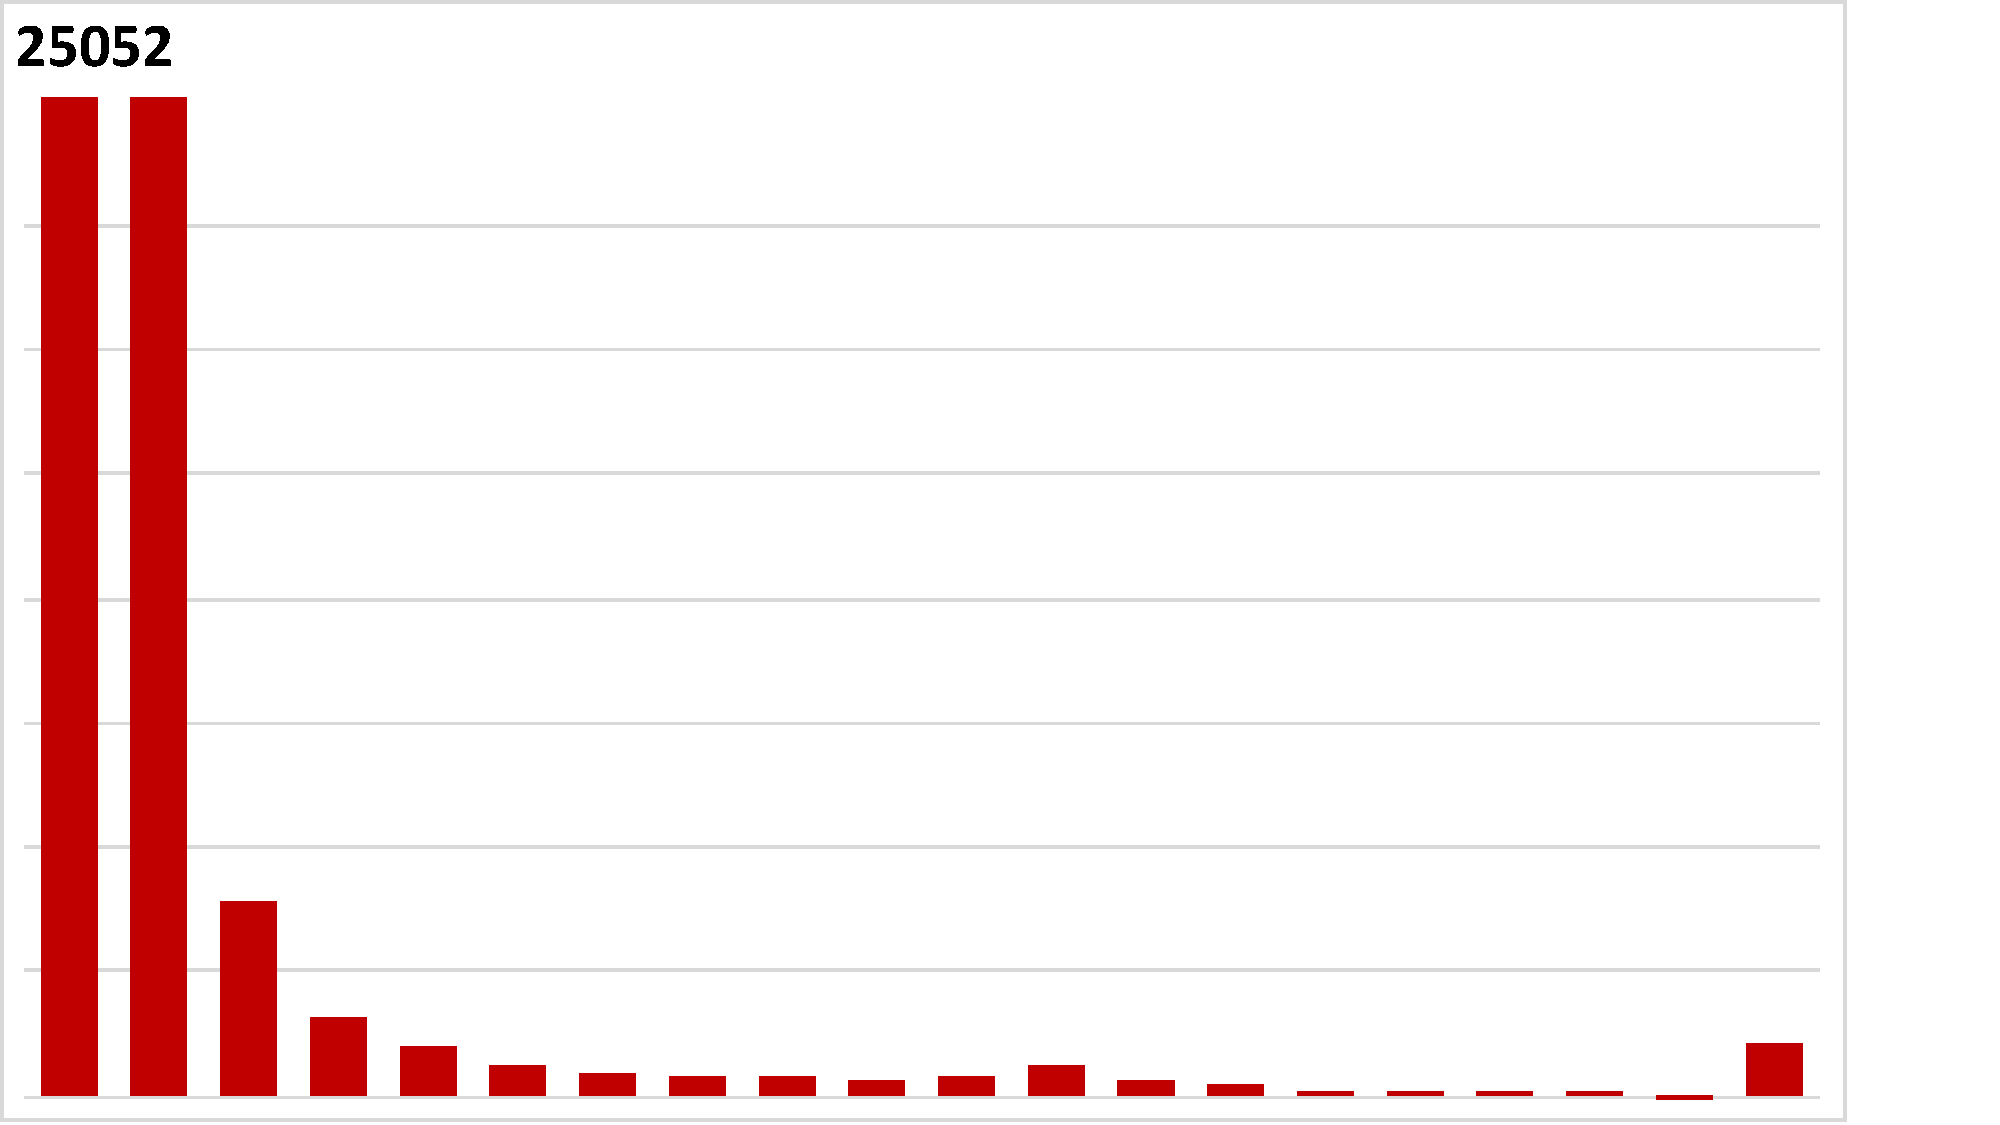
\includegraphics[width=0.95\linewidth, trim={0cm 0cm 2.5cm 0cm}, clip]{results/nyx/Lag25_1_AvgL2.pdf}
\vspace{-2mm}
\captionof{subfigure}{Lag 25 Avg$_{L2}$}
\end{minipage}%
\hfill
\begin{minipage}[t]{0.24\textwidth}%
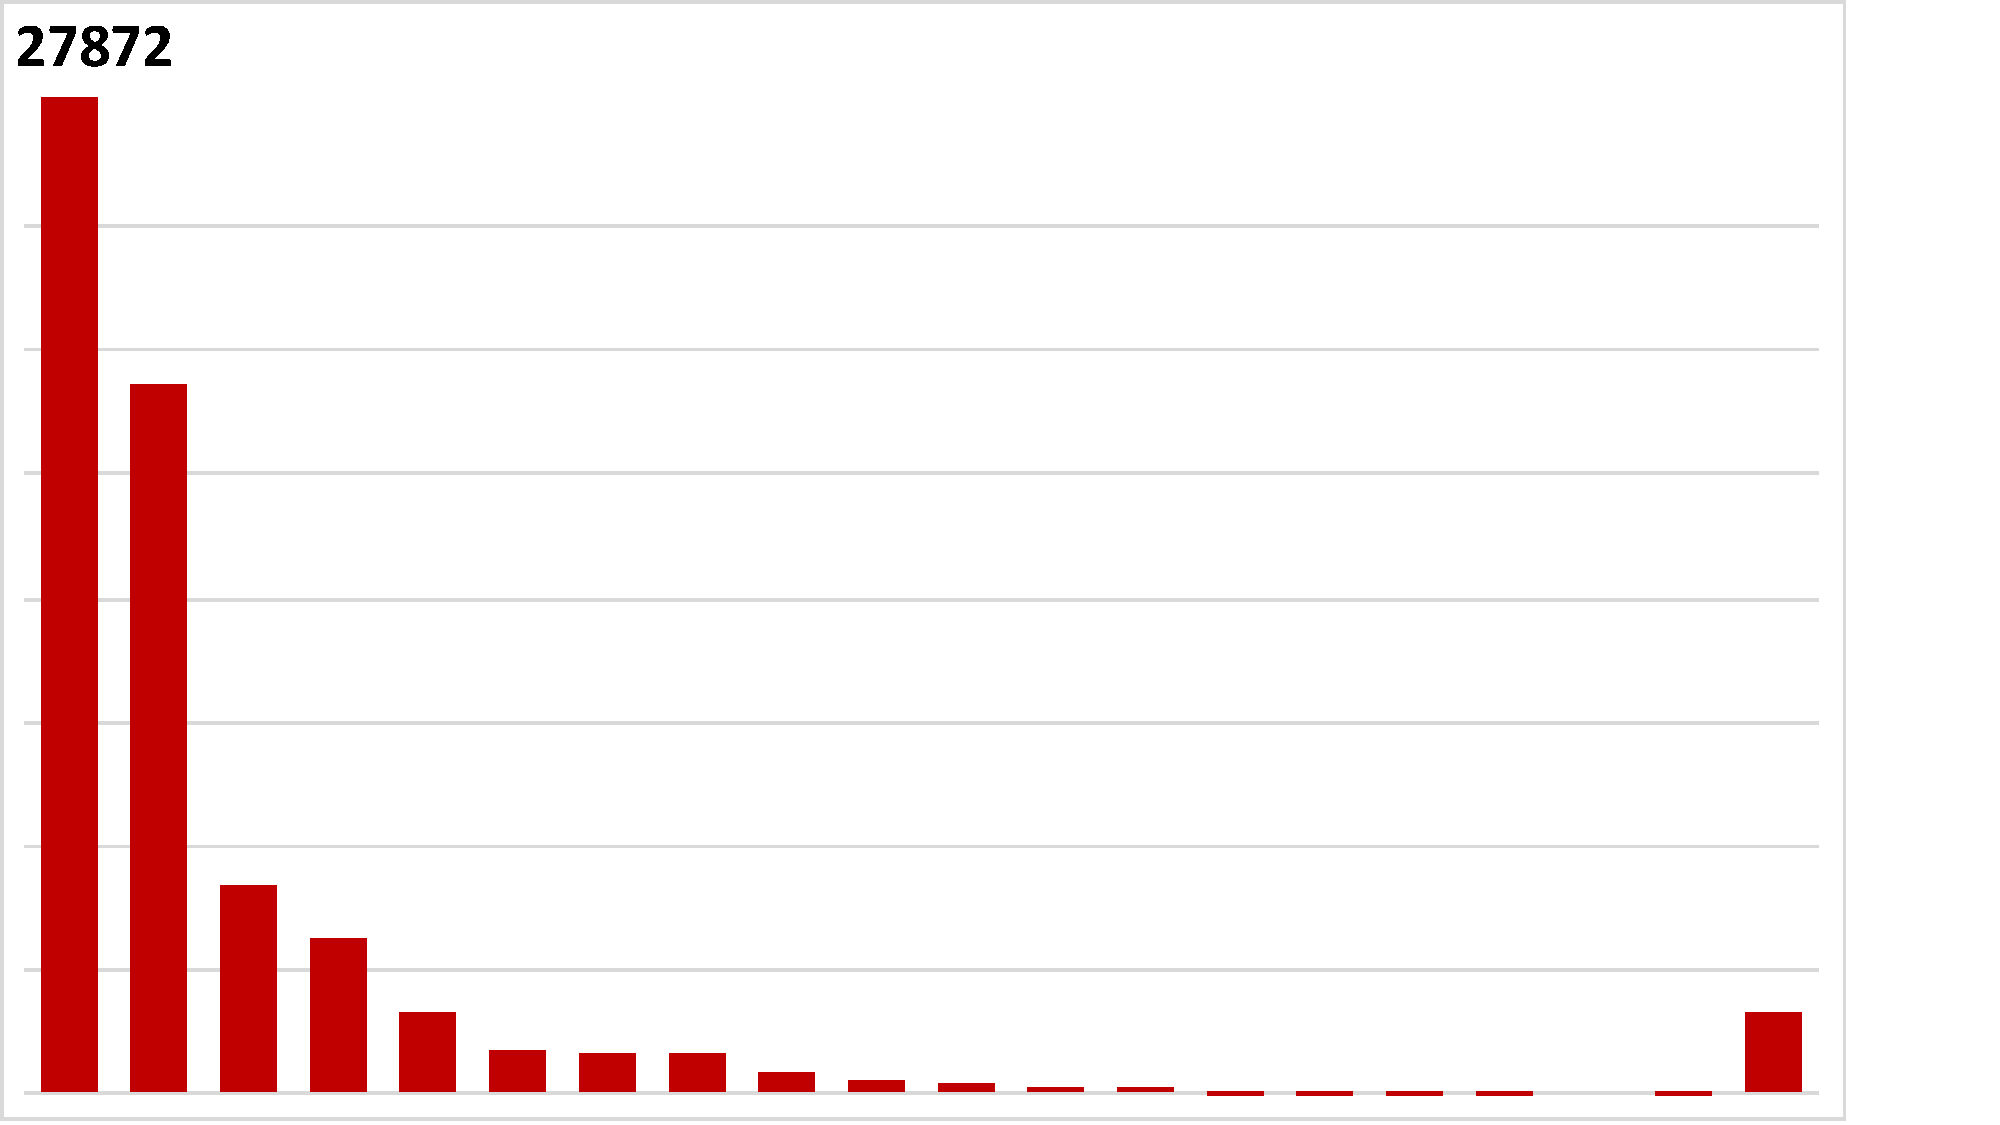
\includegraphics[width=0.95\linewidth, trim={0cm 0cm 2.5cm 0cm}, clip]{results/nyx/Lag50_1_AvgL2.pdf}
\vspace{-2mm}
\captionof{subfigure}{Lag 50 Avg$_{L2}$}
\end{minipage}
\begin{minipage}[t]{0.24\textwidth}%
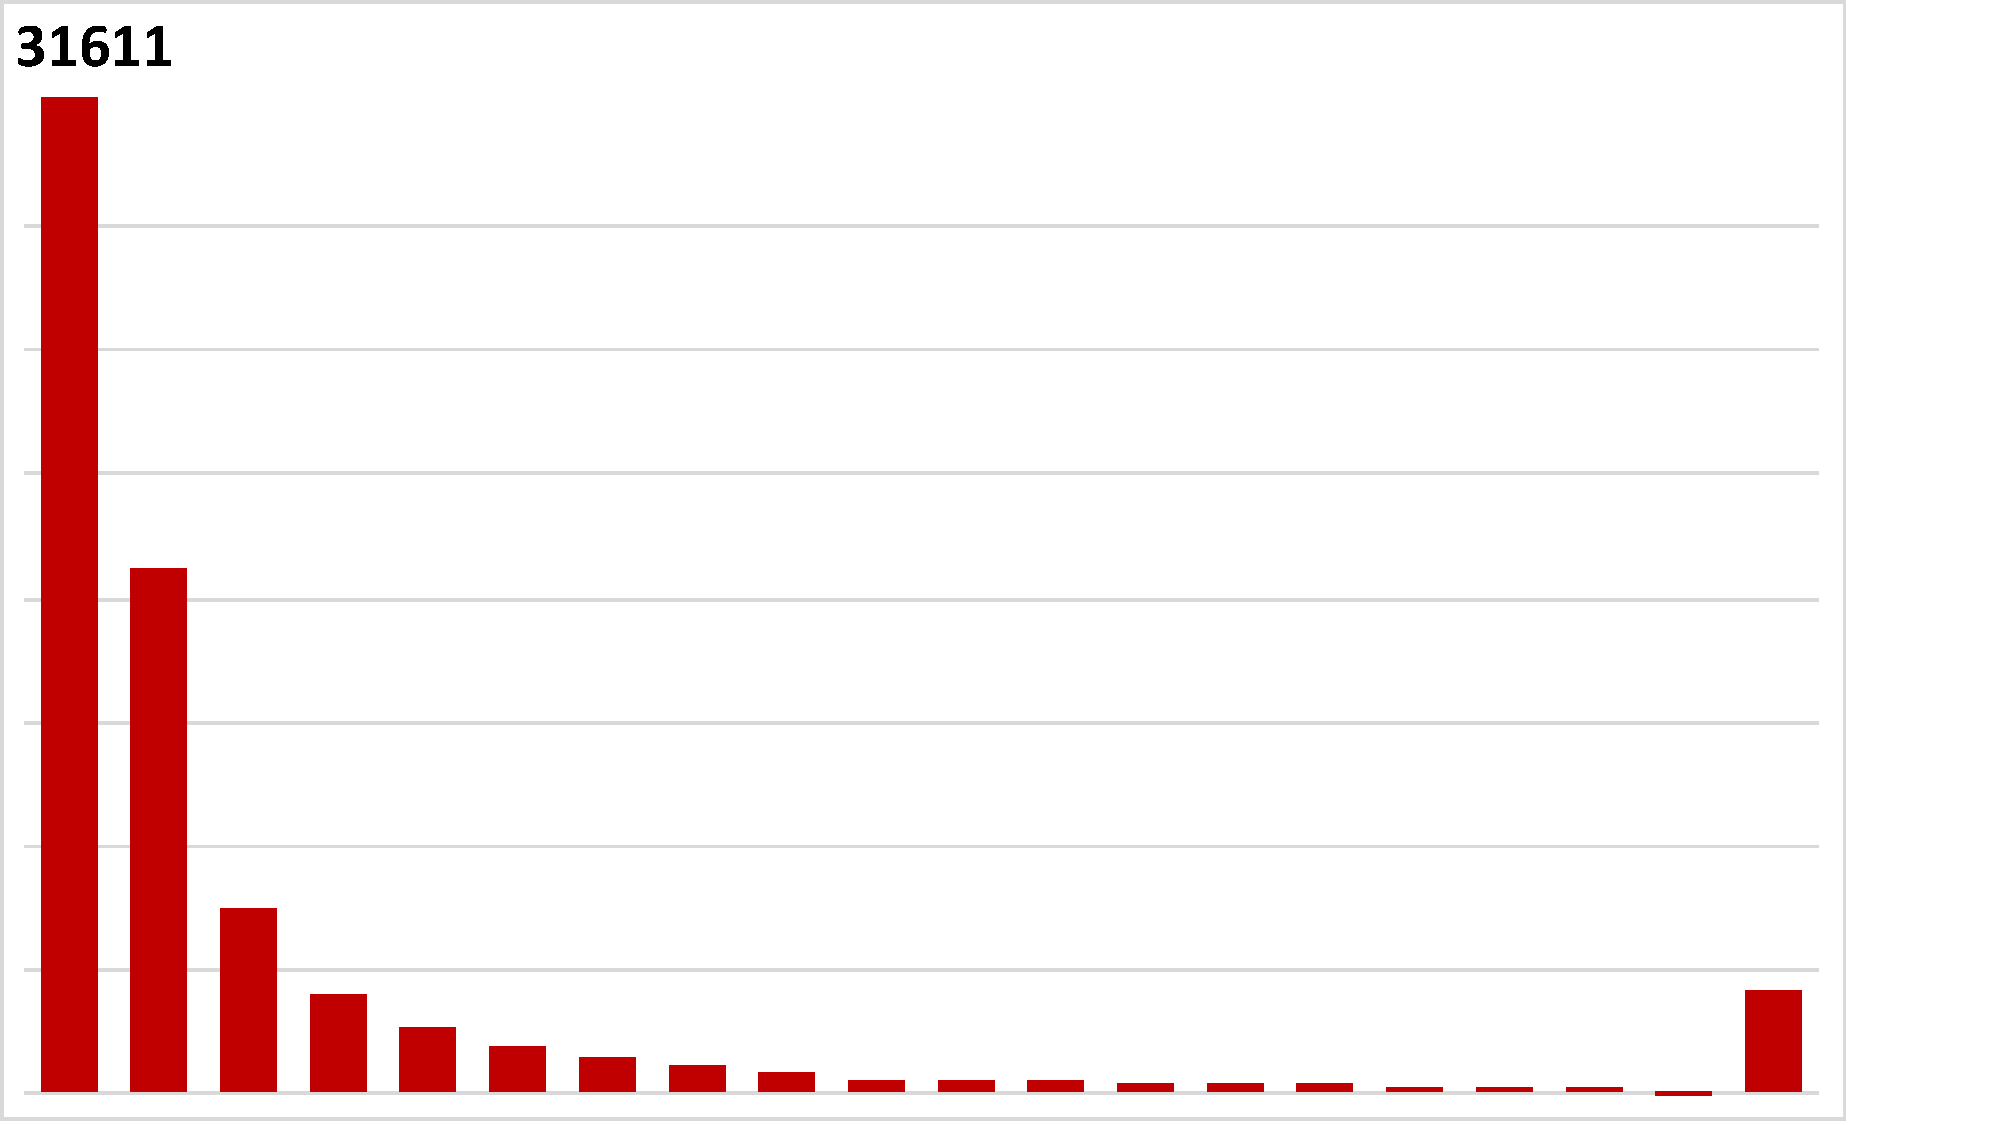
\includegraphics[width=0.95\linewidth, trim={0cm 0cm 2.5cm 0cm}, clip]{results/nyx/Lag100_1_AvgL2.pdf}
\vspace{-2mm}
\captionof{subfigure}{Lag 100 Avg$_{L2}$}
\end{minipage}%
\hfill
\begin{minipage}[t]{0.24\textwidth}%
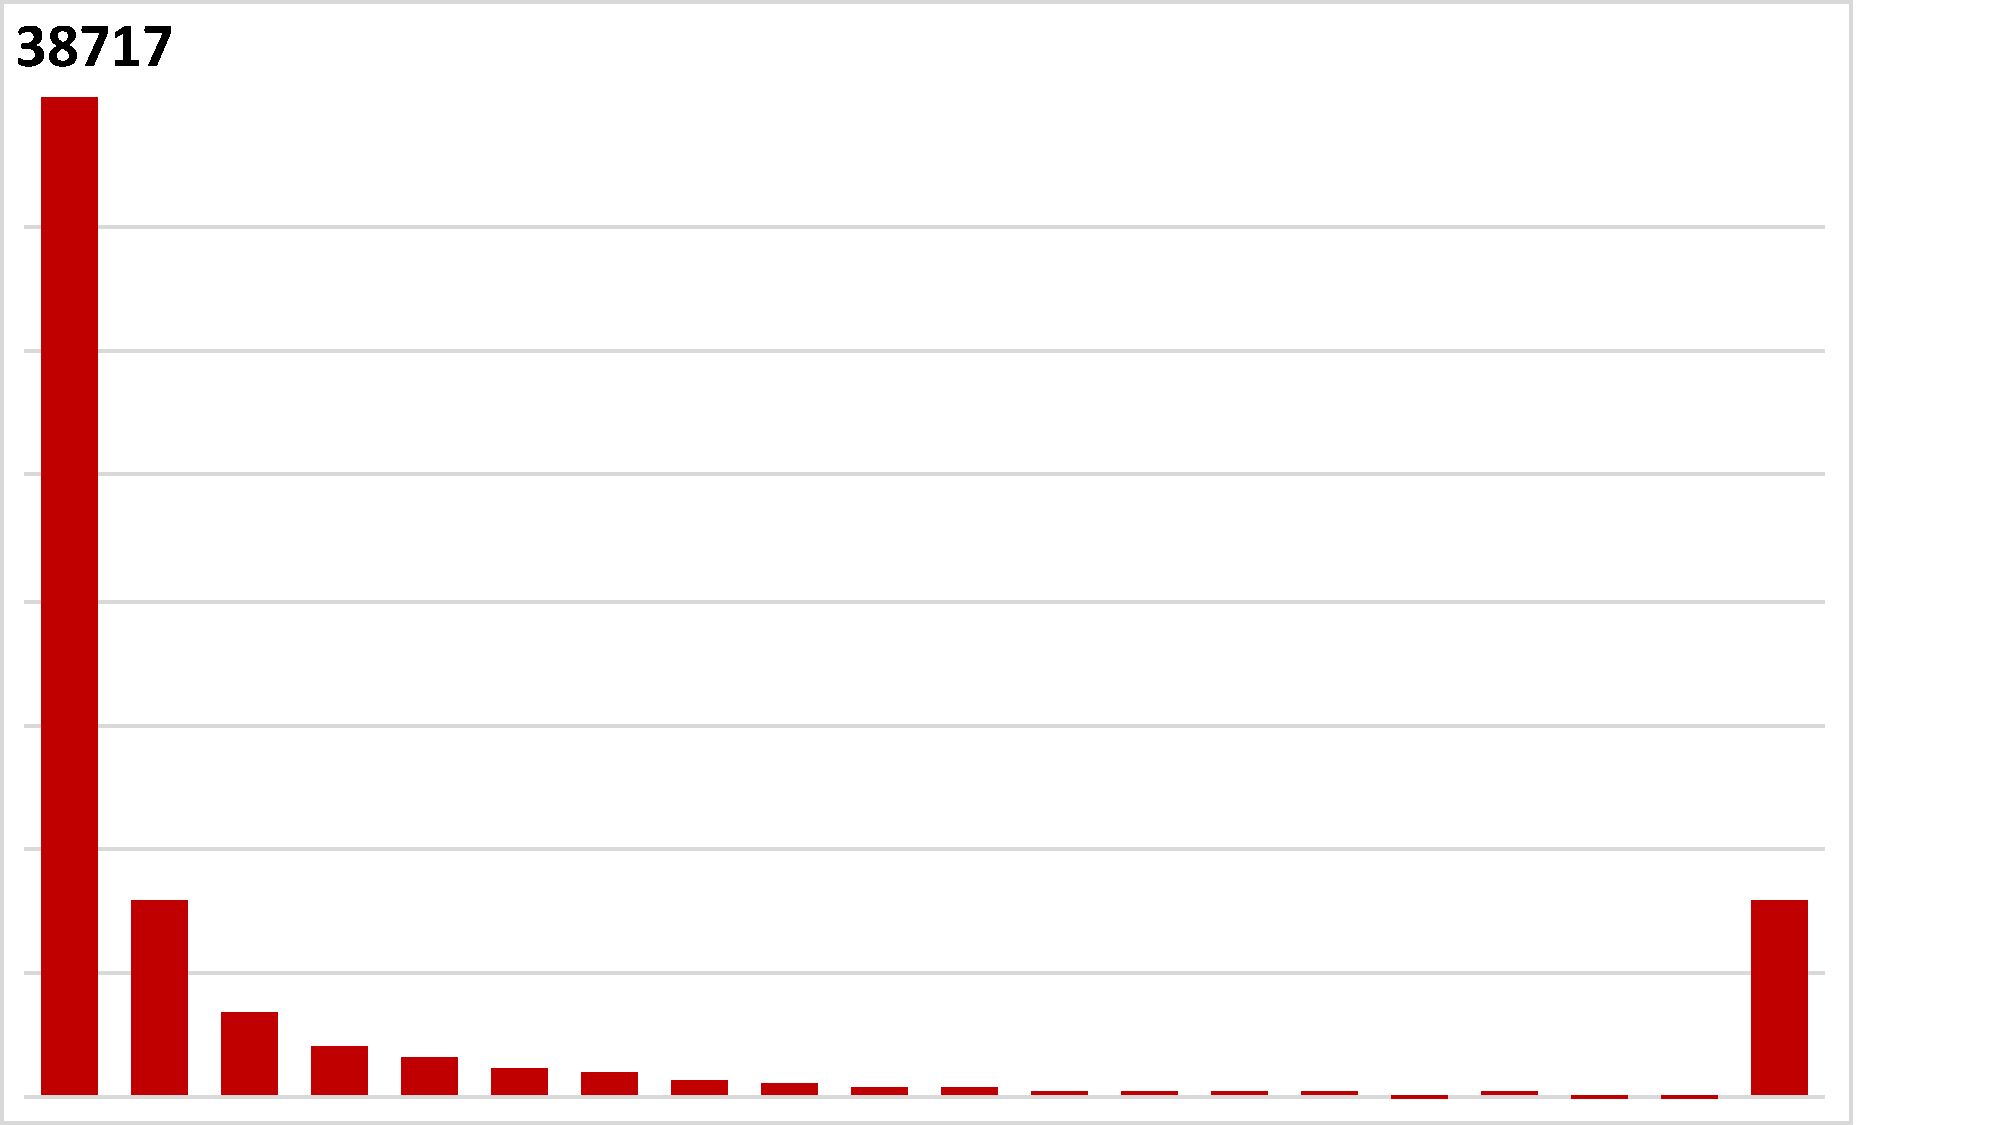
\includegraphics[width=0.95\linewidth, trim={0cm 0cm 2.5cm 0cm}, clip]{results/nyx/Lag200_1_AvgL2.pdf}
\vspace{-2mm}
\captionof{subfigure}{Lag 200 Avg$_{L2}$}
\end{minipage}
\begin{minipage}[t]{0.24\textwidth}%
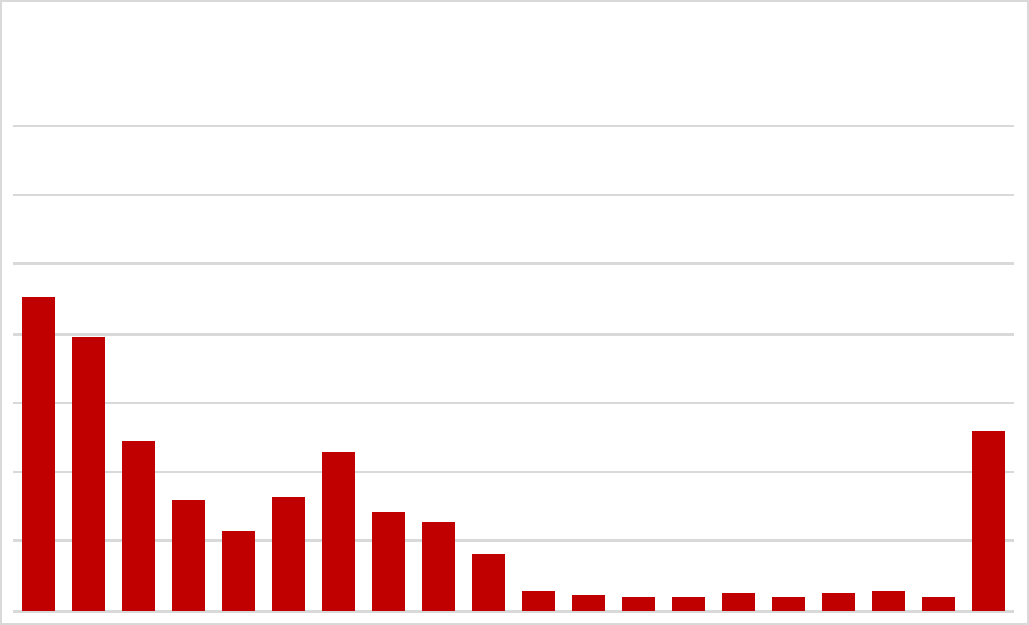
\includegraphics[width=0.95\linewidth, trim={0cm 0cm 2.5cm 0cm}, clip]{results/nyx/Lag25_1_Max.pdf}
\vspace{-2mm}
\captionof{subfigure}{Lag 25 Max$_{L2}$}
\end{minipage}%
\hfill
\begin{minipage}[t]{0.24\textwidth}%
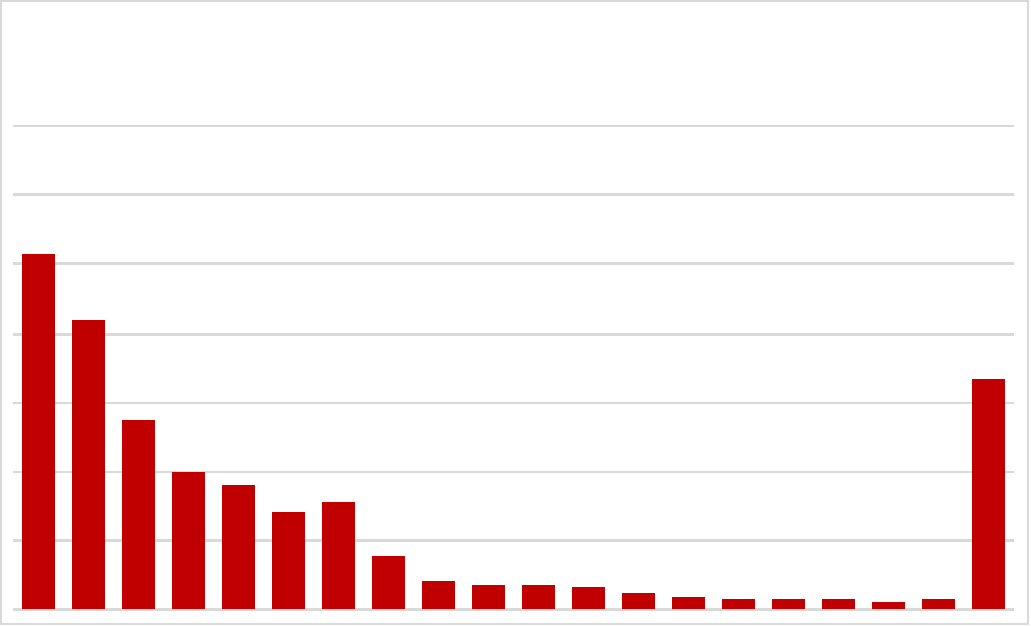
\includegraphics[width=0.95\linewidth, trim={0cm 0cm 2.5cm 0cm}, clip]{results/nyx/Lag50_1_Max.pdf}
\vspace{-2mm}
\captionof{subfigure}{Lag 50 Max$_{L2}$}
\end{minipage}
\begin{minipage}[t]{0.24\textwidth}%
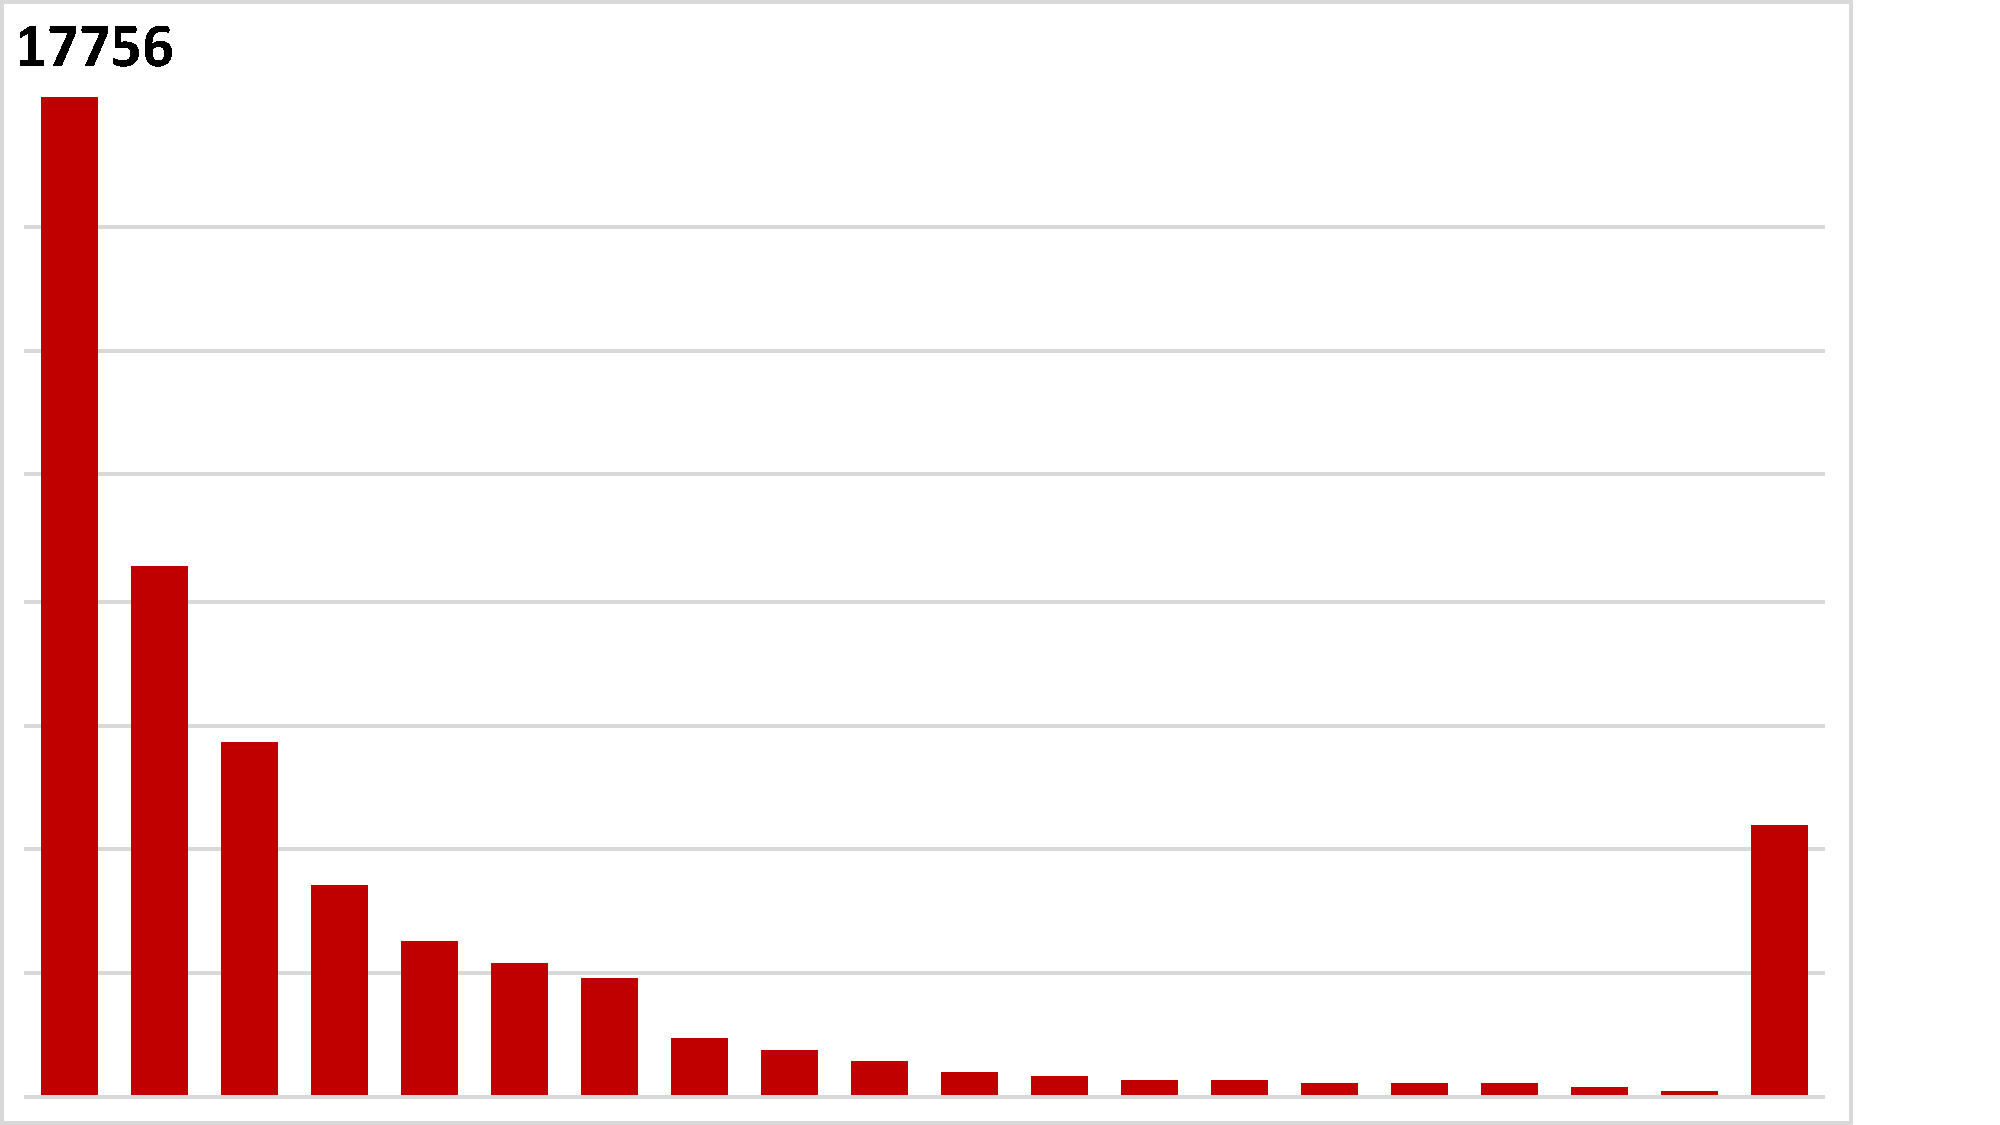
\includegraphics[width=0.95\linewidth, trim={0cm 0cm 2.5cm 0cm}, clip]{results/nyx/Lag100_1_Max.pdf}
\vspace{-2mm}
\captionof{subfigure}{Lag 100 Max$_{L2}$}
\end{minipage}%
\hfill
\begin{minipage}[t]{0.24\textwidth}%
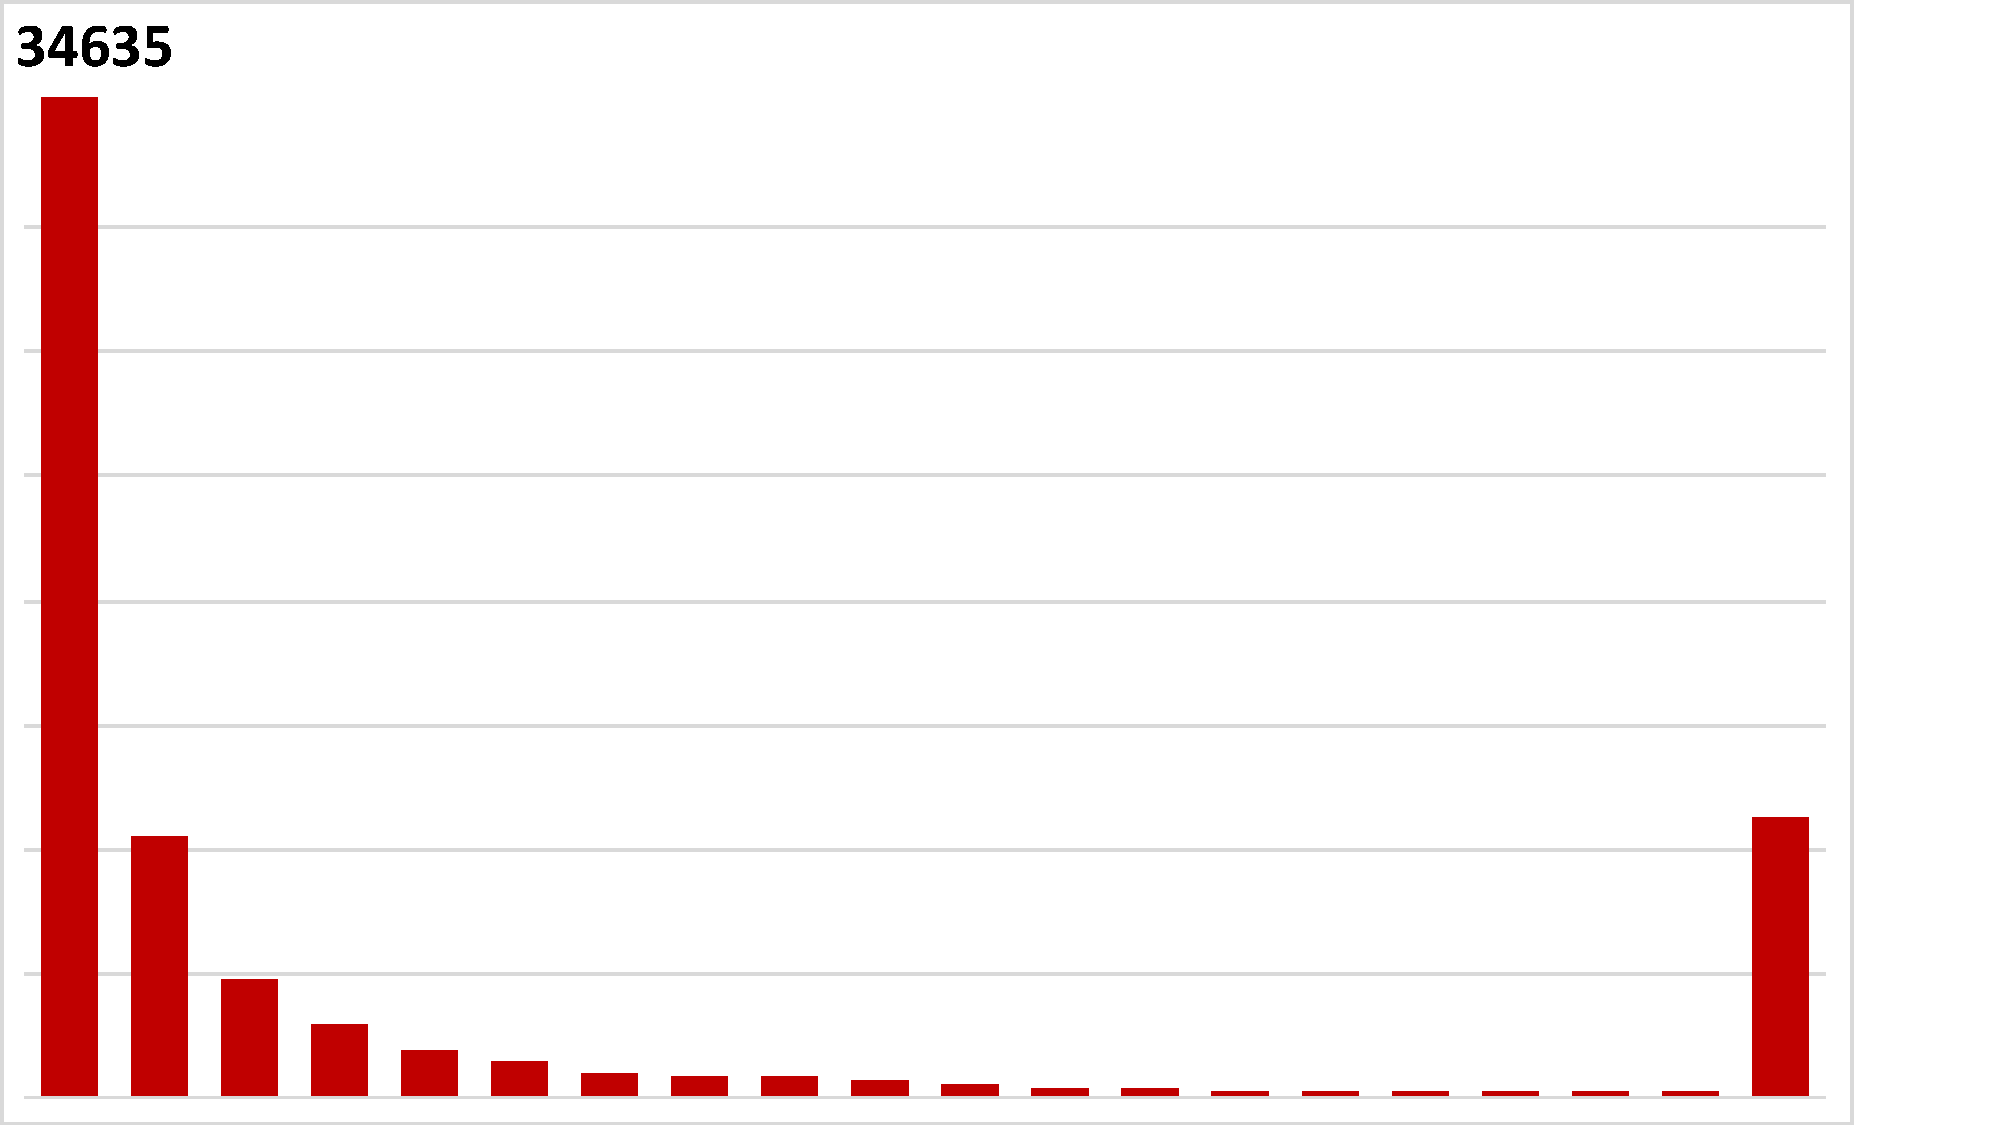
\includegraphics[width=0.95\linewidth, trim={0cm 0cm 2.5cm 0cm}, clip]{results/nyx/Lag200_1_Max.pdf}
\vspace{-2mm}
\captionof{subfigure}{Lag 200 Max$_{L2}$}
\end{minipage}
\end{framed}
\vspace{-2mm}
\captionof{figure}{\textbf{Nyx} experiment histograms for 50,000 test particle interpolation errors. Each plot has 20 bins, ranging from 0 to $>$0.44, with bar height encoding number of particles. Horizontal grid lines mark increments of 2,000.}
\label{fig:nyx_histograms}
\end{minipage}%
\vspace{-6mm}
\end{figure*}


An interesting outcome of these experiments was observing \textbf{PHE-1}, i.e., accuracy, given the variation in interval.
%
The Eulerian technique is nearly perfectly accurate when the sampling is less sparse (interval = 25).
%
In contrast, the Lagrangian technique is less accurate, even when using the same number of particles as grid points.
%
Such behavior is expected when the variation between the vector field across cycles is very small (Figure~\ref{fig:vectorfield_nyx}).
%
In such a setting, using only a fourth-order Runge Kutta (RK4) provides more accurate interpolation than applying a second-order barycentric coordinates interpolation on top of the trajectories extracted using RK4.
%
This ``stitching'' error has been studied in several prior works~\cite{hlawatsch2011hierarchical,bujack2015lagrangian,hummel2016error, sane2019interpolation}.
\begin{figure}[t]
\centering
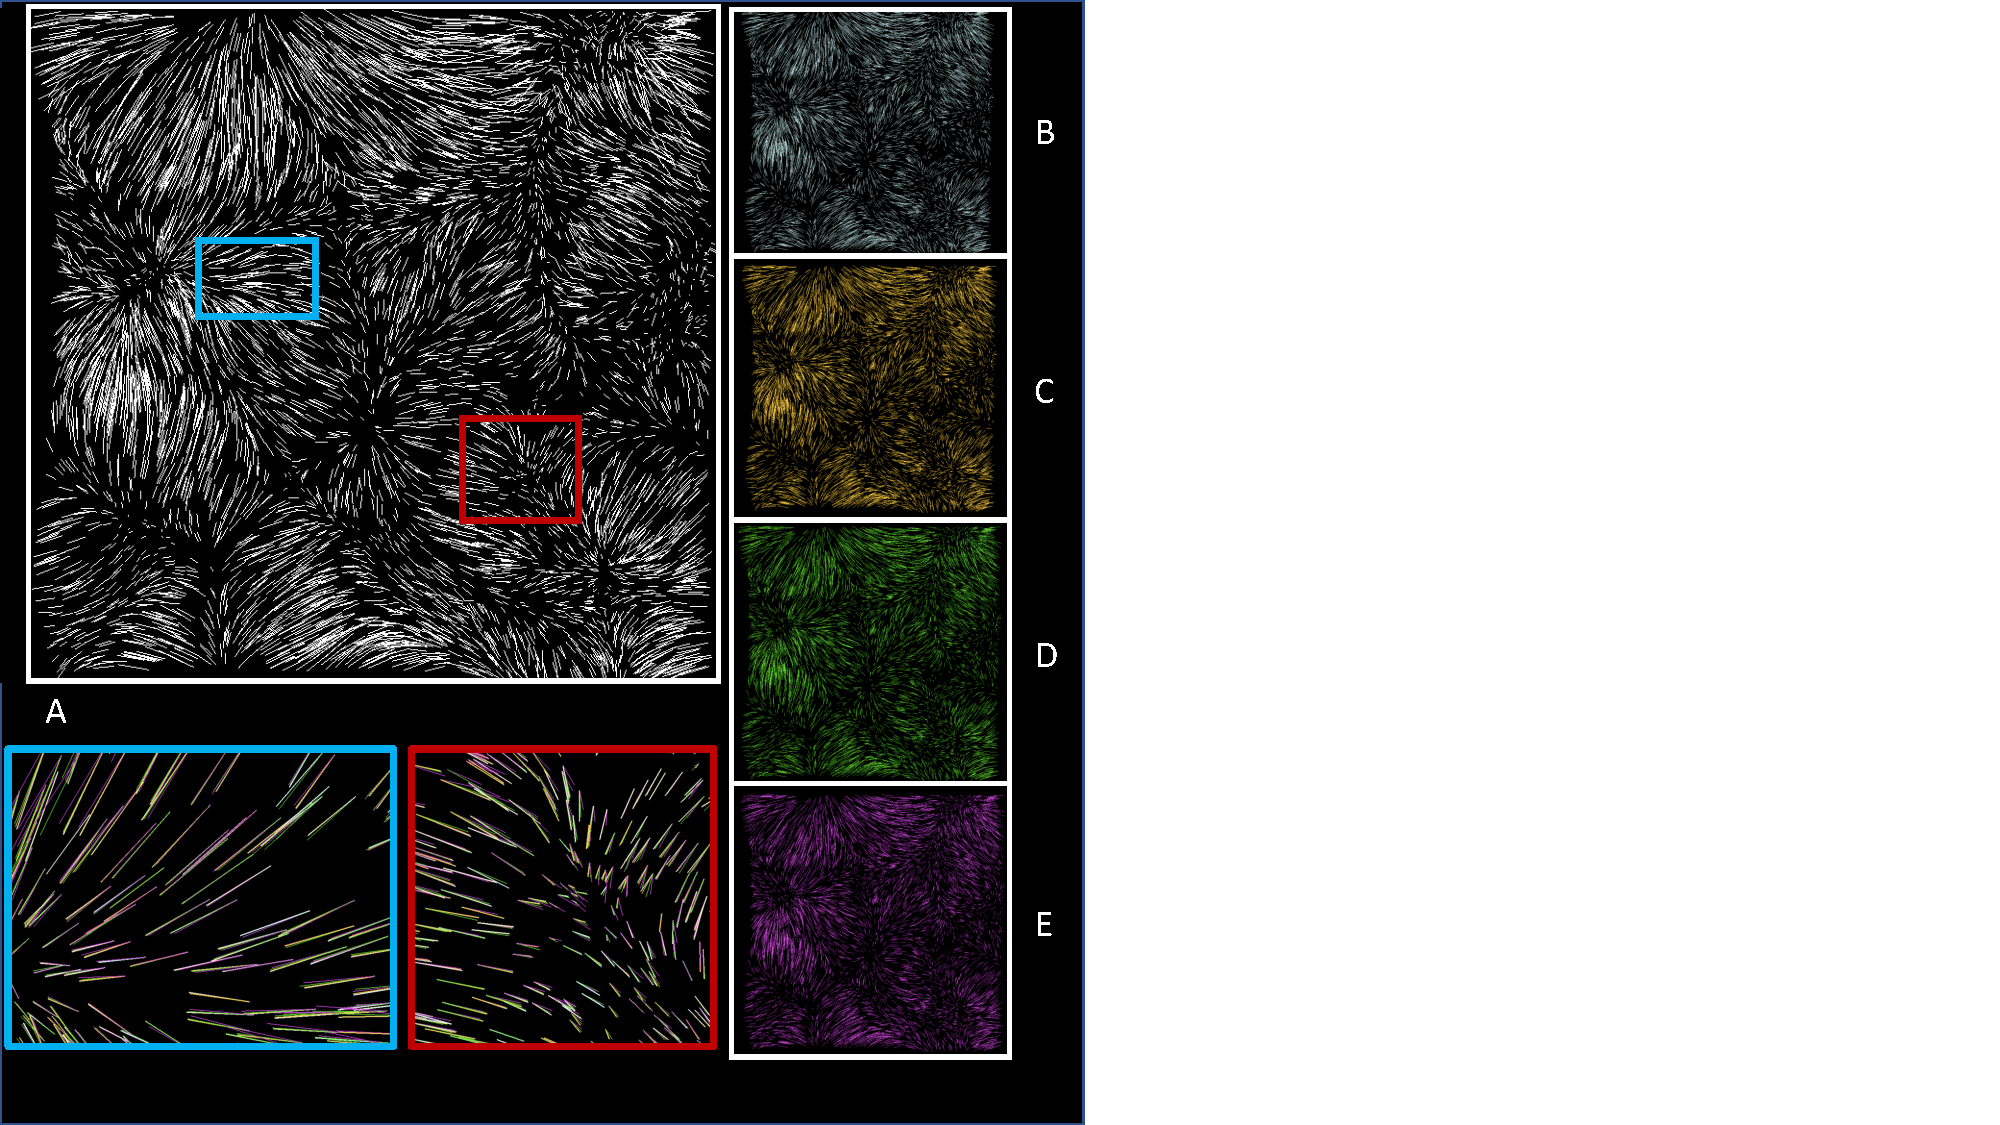
\includegraphics[width=0.87\linewidth, trim={0cm 1cm 15.5cm 0cm}, clip]{images/Nyx_Vis.pdf}
\vspace{-3mm}
\caption{A qualitative comparison of pathlets reconstructed over one interval for the Nyx data (\textbf{Interval = 25} case). For each configuration we specify \textbf{DS-1} and \textbf{PHE-1} as (Bytes, Cell Side\%). Image A (white) is the ground truth, B~(light-blue) is Eulerian~(227MB; 2.29\%), C~(yellow) is Lagrangian 1:1~(232MB; 11.61\%), D~(green) is Lagrangian 1:8~(27MB; 37.27\%), E~(pink) is Lagrangian 1:27~(8MB; 72.727\%).} 
\label{fig:nyx_vis}
\vspace{-5mm}
\end{figure}


As the interval size increases, i.e., the \textbf{S}parsity component of the \textbf{EUS} problem, we observe Lagrangian improving in accuracy and offering multiple favorable data storage-accuracy propositions.
%
For example, for an interval of 200, greater accuracy can be achieved by the Lagrangian technique using a 10X data reduction.
%
The behavior of techniques (one losing integrity as sparsity increases; another becoming more accurate as sparsity increases) is well captured by the histograms in Figure~\ref{fig:nyx_histograms}.
%
Of course, a longer interval does not guarantee better accuracy for the Lagrangian technique in all settings.
%
Divergence over a long interval impacts Lagrangian-based interpolation accuracy~\cite{chandler2016analysis}.

With respect to the impact of number of particles on \textbf{PHE-1} and \textbf{DS-1}, we observe that error increases due to data reductions are higher when the interval is smaller. 
%
For example, error increases by 3X for a 27X data reduction for interval 200 and error increases by over 6X for a 27X data reduction for interval 25.
%
We note that in each of these cases, the increases in error resulted in \textbf{AvgN$_{L2}$} values that still indicate that the majority of test particles were within the same cell as the ground truth particle.
%
This result supports the notion that the Lagrangian technique can effectively support data reduction in settings of temporal sparsity.
%
Overall, our empirical study using the derived Nyx vector field produced interesting trends that support the use of Lagrangian technique for \textbf{EUS} problem, while also demonstrating a stitching error when storing data to disk more frequently.

